\documentclass[11pt]{article}
\usepackage[T1]{fontenc}
\usepackage{lmodern,microtype}
\usepackage{amsmath,amssymb,amsthm,mathrsfs,mathtools,booktabs,array,longtable}
\usepackage[margin=1in]{geometry}
\usepackage{tikz}
\usetikzlibrary{positioning,arrows.meta}
\usepackage[hyphens]{url}
\usepackage{hyperref}
\hypersetup{colorlinks=true,linkcolor=blue!45!black,citecolor=blue!45!black,urlcolor=blue!45!black,pdftitle={Integer multiplication below n log n},pdfauthor={OpenAI}}
\pdfinfoomitdate=1
\pdftrailerid{}
\pdfsuppressptexinfo=15
\newtheorem{theorem}{Theorem}
\newtheorem{lemma}[theorem]{Lemma}
\newtheorem{proposition}[theorem]{Proposition}
\newtheorem{corollary}[theorem]{Corollary}
\theoremstyle{definition}
\newtheorem{definition}[theorem]{Definition}
\newtheorem{remark}[theorem]{Remark}
\newcommand{\norm}[1]{\lVert#1\rVert_\infty}
\title{Integer multiplication below \texorpdfstring{$n\log n$}{n log n}}
\author{OpenAI}
\date{September 23, 2026}
\begin{document}
\maketitle
\begin{abstract}
We give a deterministic algorithm that multiplies two $n$-bit integers
in $O(n(\lg n)^{1-\kappa})$ worst-case time, with
$\kappa=2^{-182}$, on one fixed finite-alphabet Turing machine with a
fixed finite number of one-dimensional tapes. The algorithm is exact
for every input length and disproves the $n\log n$ optimality conjecture
of Sch\"onhage and Strassen in this model.
\end{abstract}
\tableofcontents
\clearpage
\section{Introduction}

Sch\"onhage and Strassen proved in 1971 that two $n$-bit integers can
be multiplied in $O(n\log n\log\log n)$ time on a multitape Turing
machine, and proposed $n\log n$ as the optimal order of growth
\cite[Section~1]{SchonhageStrassen1971}. After a sequence of improvements,
Harvey and van der Hoeven reached the unconditional $O(n\log n)$ upper
bound~\cite{HarveyHoeven2021}. We obtain a strict power saving in the
logarithmic factor, in the same fixed finite-tape model. The algorithm
uses linear combinations of intermediate data to reduce the cost of
both address rearrangement and Fourier-transform layers.

For a binary string $x$ of length $n$, let $\operatorname{val}(x)$ be
its nonnegative integer value, with the leftmost bit most significant.
For $0\le z<2^k$, let $\operatorname{bin}_k(z)$ denote its binary
representation padded on the left to length $k$. We consider exact
multiplication: on input $x\#y$, with $x,y\in\{0,1\}^n$, the output
must be $\operatorname{bin}_{2n}(\operatorname{val}(x)\operatorname{val}(y))$.
Write $\lg n=\max\{\lceil\log_2 n\rceil,1\}$.

\begin{theorem}\label{thm:main}
There is one deterministic Turing machine $A$, with a fixed finite
alphabet and a fixed finite number of one-dimensional tapes, that
computes this exact product for every $n\ge1$ and every pair of $n$-bit
inputs. Its worst-case running time satisfies
\[
 T_A(n)=O\!\left(n(\lg n)^{1-\kappa}\right),
 \qquad \kappa=2^{-182}.
\]
\end{theorem}

The bound is asymptotic through all input lengths. The constants and
thresholds in the construction are extremely large; the algorithm is
intended to establish a bit-complexity bound. The theorem refutes an
eventual $\Omega(n\log n)$ lower bound for every fixed multiplication
machine in this model.

\subsection{The two tape operations}

Splitting the inputs into radix digits reduces multiplication to
convolution of short integer coefficients. Our starting point is the
Gaussian-resampling reduction of Harvey and van der Hoeven
\cite{HarveyHoeven2021}: it replaces the Fourier transforms needed for
this convolution by multidimensional transforms whose axis lengths are
powers of two. After a further conversion to convolution, one coordinate
is stored as the coefficient list of a polynomial modulo $y^r+1$, with $r$ a power of two. Powers of $y$ then
serve as roots of unity in the remaining axes, and multiplication by
such a root is a signed shift of the coefficient list. These are the
synthetic polynomial transforms of Nussbaumer and Quandalle and
Nussbaumer~\cite{NussbaumerQuandalle1978,Nussbaumer1980}.

In this representation, the transform calculation consists of address
rearrangements, signed shifts, and two-point butterfly operations.
Scanning an array of $\Theta(n)$ stored bits at each of
$\Theta(\log n)$ transform levels already costs $\Theta(n\log n)$.
We therefore need savings in both movement and arithmetic. Two tape
procedures supply them; in both bounds, $V$ denotes the stored bit volume.

The first procedure interchanges two disjoint contiguous address fields
of $u$ bits in an array whose addresses form a complete Cartesian
product. Its cost is $O(Vu^\tau)$ for a fixed $\tau<1$.
Although its final effect is an exact permutation, its intermediate
steps form pointwise XOR combinations of data. The final permutation is
exact for arbitrary initial auxiliary values.

The second procedure applies
\[
 H_0(u,v)=\bigl((u+v)/2,(u-v)/2\bigr)
\]
simultaneously on selected coordinate bits of the numerical arrays.
Each record is a polynomial with complex fixed-point coefficients, and
$H_0$ acts coefficientwise. On the layouts used in the multiplication
algorithm, one selects the same bit position in each of at most $d$
equal-width address chunks, and the cost is $O(Vd^{\lambda'})$ for a
fixed $\lambda'<1$. Intermediate values are exact Gaussian dyadics,
whose real and imaginary parts have power-of-two denominators. A single
truncation follows the completed contractive layer.
Section~\ref{sec:tape-interchange} proves the address bound, and
Section~\ref{sec:fast-butterfly-layers} gives the numerical layout,
precision hypotheses, and layer bound.

\subsection{Linear networks and the recursive saving}

Each procedure arises from its own fixed linear network that exchanges two
banks of values, with prescribed signs, and restores every auxiliary
value. A wire's fixed place in the network is called its role. To use
the network on an array, regard a row as the complete ordered suffix,
including all active address fields, at a fixed prefix and row index.
Distribute rows cyclically among the $W$ roles, padding the row count
for each prefix to a multiple of $W$. Let $V$ now denote the node volume
after padding. All role streams have the same local address set and each
contains $V/W$ bits. A scalar gate is then applied
pointwise to matching addresses on the roles that it touches.

The representation of a role's array may change along the network.
At a source, gate, or sink $v$, choose an invertible linear operator
$D_v$ on the space of arrays indexed by the common address set. We call $D_v$ its frame: the stored
array is $D_vg$ when the logical array is $g$. All incidences of one
gate have the same frame. Along an edge from $u$ to $v$, the operator
$D_vD_u^{-1}$ changes the stored array from $D_ug$ to $D_vg$.
At a pointwise linear gate $G$, the common frame commutes with the gate:
\[
 G(D_vg_1,\ldots,D_vg_t)=D_vG(g_1,\ldots,g_t).
\]
The supplied input needs no preliminary change of frame: its logical
interpretation is defined by applying the inverse input frame. Thus the
intermediate frames cancel, and a route from input role $w$ to output
role $\rho(w)$ applies
$D_{\mathrm{sink}(\rho(w))}D_{\mathrm{source}(w)}^{-1}$, together with
its prescribed scalar sign. Undoing the role exchange and those signs
leaves the endpoint operator on every role array, including the roles
that carried auxiliary scalar values.

For the bit procedure, that endpoint operator is an address shear:
two fields, written as vectors $H,D$ over a common residue ring, are
updated by $(H,D)\mapsto(H+D,D)$. Two further linear-cost address
updates complete their interchange. For the numerical procedure, the
endpoint operator becomes the simultaneous $H_0$ layer after diagonal
phase operations and a dyadic scale. The intermediate frames are chosen
so that every edge can be implemented by smaller calls to the same
procedure.

The finite construction in Section~\ref{sec:finite-networks} attaches
subspaces of a fixed $m$-dimensional space to its gates and terminals.
The subspaces at adjacent vertices are nested. Their dimension changes
count the smaller operations needed on an edge, with an additional
source contribution in the bit construction. The construction uses
three-element subsets: gather and scatter create coefficients depending
on intersection size, and auxiliary wires cancel the unwanted
coefficients. Orthogonality of the corresponding indicator vectors permits
the subspace assignments. The decisive property is that the total
number $s$ of smaller calls satisfies $s<Wm$.

A recursive call at parameter $mf$ therefore uses $s$ calls at parameter
$f$, each on a stream of volume $V/W$. The parameter counts field
digits for address interchange and selected axes for a numerical layer.
After dividing cost by volume, multiplying the parameter by $m$
increases the recursive contribution by $s/W<m$. This strict inequality
is the source of the power saving. The later tape and arithmetic
estimates preserve it, including the work of changing numerical address
coordinates. Those changes are implemented by whole-chunk moves and
controlled shifts, followed by a deterministic correction of the
explicitly identified exceptional addresses.

\subsection{From transforms to the exact product}

The remaining proof places these procedures inside the multiplication
reduction and accounts for every change of representation.
First, the radix-digit coefficient list is placed on a product of
distinct prime cyclic axes by a Chinese-remainder map that preserves
convolution. Section~\ref{sec:assembly} implements this map through
triangular controlled shifts and charged axis moves. Gaussian
resampling then expresses each source Fourier transform through a
power-of-two tensor transform. Section~\ref{sec:resampling} retains the
source and target coordinate permutations in the transform identity,
so they need not be executed as separate full sorts.

Next, Bluestein's chirp identity converts the middle transform,
including its target permutation, into normalized cyclic convolution.
A phase twist changes the last cyclic coordinate into a polynomial
modulo $y^r+1$; its negative wrap gives precisely the original cyclic
wrap after the twist is removed. Sections~\ref{sec:synthetic-layouts}
and~\ref{sec:exact-ring-products} compute convolution on the remaining
axes over this polynomial ring. The two forward synthetic transforms
retain the same frequency order through their pointwise product, and
the opposite transform consumes that order. Their polynomial products
use signed packing and the established $O(n\log n)$ multiplier as an
ordinary subroutine.

Finally, the source permutation retained during resampling cancels
across the two forward source transforms, their pointwise product,
and the opposite-sign transform. Section~\ref{sec:assembly} removes
the known normalizations and digit scales, proves that the recovered
coefficient error is strictly below $1/2$, and propagates carries to
obtain the exact binary product. A compatible choice of rational
parameters makes all terms in its cost table fit Theorem~\ref{thm:main}.
Figure~\ref{fig:multiplication-flow} summarizes these reductions.

\begin{figure}[ht]
\centering
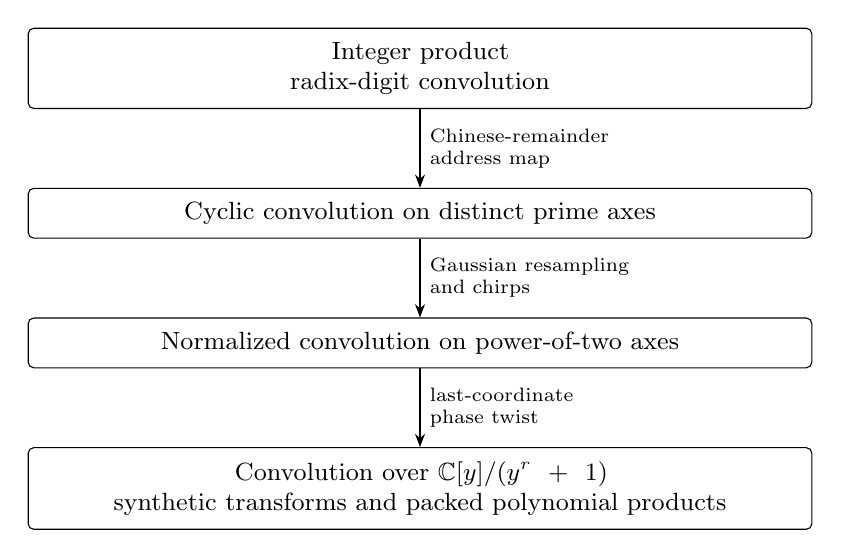
\begin{tikzpicture}[
 node distance=10mm,
 every node/.style={font=\small},
 box/.style={draw,rounded corners=2pt,align=center,text width=9.6cm,inner sep=5pt},
 >=Stealth]
\node[box] (digits) {Integer product\\radix-digit convolution};
\node[box,below=of digits] (prime) {Cyclic convolution on distinct prime axes};
\node[box,below=of prime] (power) {Normalized convolution on power-of-two axes};
\node[box,below=of power] (ring) {Convolution over $\mathbb C[y]/(y^r+1)$\\
synthetic transforms and packed polynomial products};
\draw[->] (digits)--node[right,font=\scriptsize,align=left]
 {Chinese-remainder\\address map}(prime);
\draw[->] (prime)--node[right,font=\scriptsize,align=left]
 {Gaussian resampling\\and chirps}(power);
\draw[->] (power)--node[right,font=\scriptsize,align=left]
 {last-coordinate\\phase twist}(ring);
\end{tikzpicture}

\caption{The reductions connecting the tape procedures to multiplication.
The arrows describe changes of problem and representation. Fast address
interchanges organize the layouts, and simultaneous butterfly layers
accelerate the synthetic transforms. Solving the final polynomial-ring
convolution evaluates the transforms needed in the preceding stages.
Known rescalings, rounding, and carry propagation then recover the exact
integer product.}
\label{fig:multiplication-flow}
\end{figure}

\subsection{Other arithmetic operations}

\begin{corollary}[Exact division and integer square root]
\label{cor:exact-arithmetic}
There are deterministic machines with fixed finite alphabets and fixed
finite numbers of one-dimensional tapes performing the following tasks
in $O(n(\lg n)^{1-\kappa})$ worst-case time, for every $n\ge1$. For
$x,y\in\{0,1\}^n$, put $a=\operatorname{val}(x)$ and
$b=\operatorname{val}(y)$. If $b>0$, the division machine takes $x\#y$
and returns $\operatorname{bin}_n(q)\#\operatorname{bin}_n(r)$, where
$q=\lfloor a/b\rfloor$ and $r=a-bq$. The square-root machine takes $x$
and returns $\operatorname{bin}_n(\lfloor\sqrt a\rfloor)$.
Leading zeroes are allowed, and $\kappa$ is as in
Theorem~\ref{thm:main}.
\end{corollary}

The classical Newton reductions described by
Brent~\cite[Lemmas 2.1--2.4]{Brent1976} compute reciprocal and
square-root approximations at geometrically increasing precisions.
Their multiplication costs are bounded by a geometric sum controlled by
the last precision, and exact remainder and square tests recover the
required integer answers. Section~\ref{sec:exact-arithmetic-proof}
gives the complete fixed-tape implementation.


\subsection{Historical context and inherited methods}

Karatsuba's recursive construction, published jointly
with Ofman in 1962, gave a binary multiplication circuit of size
$O(n^{\log_2 3})$~\cite{KaratsubaOfman1962}. Toom's subsequent use of polynomial
evaluation and interpolation gave circuit size
$n\exp(O(\sqrt{\log n}))$, and hence $O(n^{1+\eta})$ for every fixed
$\eta>0$~\cite{Toom1963}. These early results were formulated in terms of
automata and logical networks. Cook adapted Toom's method to the
Turing-machine setting; the contemporary account of Sch\"onhage and
Strassen credits this adaptation explicitly
\cite[Section~1, p.~282]{SchonhageStrassen1971}.

In the multitape Turing model,
Sch\"onhage and Strassen proved the bound
$O(n\log n\log\log n)$ in 1971~\cite{SchonhageStrassen1971}.
F\"urer improved it to $n\log n\,2^{O(\log^* n)}$ in 2007, with a full
journal account in 2009~\cite{Furer2007,Furer2009}; here $\log^* n$ counts
iterated logarithms until a constant threshold is reached.
De, Kurur, Saha and Saptharishi developed a modular-arithmetic route to
the same scale~\cite{DeKururSahaSaptharishi2013}.
Later improvements made the exponential factor $8^{\log^* n}$ and then
$4^{\log^* n}$~\cite{HarveyHoevenLecerf2016,HarveyHoeven2019Lattice}.
Harvey and van der Hoeven proved the unconditional
$O(n\log n)$ bound~\cite{HarveyHoeven2021}.

The multitape bounds just cited concern that fixed model. Sch\"onhage obtained
linear-time multiplication on storage-modification machines~\cite{Schonhage1980}.
Groff later gave a smaller-than-$\log n$ factor in a unit-cost RAM model
with constant-time arbitrary memory access, after polynomial preprocessing
whose cost is excluded from that bound~\cite[Sections~2 and~4]{Groff2019}.
Neither result establishes the bound in the fixed finite-tape model of
Theorem~\ref{thm:main}.

The transform methods behind these bounds also underlie the present
construction. Sch\"onhage--Strassen multiplication uses roots of unity in
Fermat-type residue rings, where certain multiplications become shifts.
F\"urer combines cheap polynomial roots of unity with more general roots,
reducing the frequency of expensive multiplications. Harvey and van der
Hoeven use Gaussian resampling to pass to multidimensional transforms with
power-of-two dimensions, then evaluate them using polynomial transforms
developed by Nussbaumer and Quandalle and subsequently by
Nussbaumer~\cite{NussbaumerQuandalle1978,Nussbaumer1980,HarveyHoeven2021}.
The Gaussian-gridding work of Dutt and Rokhlin is an earlier conceptual
precursor~\cite{DuttRokhlin1993}; Harvey and van der Hoeven discuss the
connection in~\cite[Section~4.4.3]{HarveyHoeven2021}. The quantitative
resampling and bit-cost estimates used here are those of the latter paper.

More specifically, the proof adapts Harvey and van der Hoeven's
Gaussian-resampling identity, contraction bounds, and short-convolution
procedures~\cite[Theorem~4.2, Proposition~4.7 and Lemmas~4.8--4.12]{HarveyHoeven2021}.
Their framework already permits arbitrary dimension. Here the source and
target permutations remain in the transform identity, while the faster tape
procedures perform the required axis movements. Bluestein's conversion to
convolution~\cite{Bluestein1970} and the synthetic-root convolution algorithm
are retained; the latter follows the polynomial-transform construction
in~\cite[Section~2.4 and Section~3]{HarveyHoeven2021}. Signed coefficient
packing is a form of Kronecker substitution, with the fixed-tape version
of~\cite[Lemma~2.5]{HarveyHoeven2021} as a direct antecedent.
Calls to the established $O(n\log n)$ multiplier are ordinary subroutine
calls; they do not invoke the improved theorem recursively.

\subsection{The finite-network ingredients}

The subset-intersection construction in Section~\ref{sec:finite-networks}
has an earlier source outside multiplication. Alon's presentation of the
Frankl--Wilson construction~\cite{FranklWilson1981} gives low-degree
representations of complementary intersection graphs over different fields
\cite[Section~3, remark after the proof of Theorem~1.1]{Alon1998}.
At the prime $p=2$, its subsets have size three and the two polynomial evaluations
are the intersection count modulo two and the intersection count minus one.
These are the two pairing formulas used here. We change the ground-set
size and express the second pairing through a rational bilinear form.

The gather and scatter operations, together with the side wires, have the
form of linear index-code decoding: a low-rank linear summary gives the
wanted coordinate plus contributions from known neighboring coordinates,
and those contributions are subtracted. Bar-Yossef, Birk, Jayram and Kol
establish the fitting-matrix formulation and this decoder
\cite[Section~3, proof of Theorem~5]{BarYossefBirkJayramKol2006}.
Lubetzky and Stav treat decoding over other fields and use related
intersection representations to separate their possible ranks
\cite[Proposition~2.1 and Section~2.3]{LubetzkyStav2009}.
These comparisons explain the algebraic role of the two fields here;
they do not supply the subspace labels on the subsequent network.

Restoring scratch registers with arbitrary initial contents also has a
precise precedent. The transparent-computation construction of Buhrman,
Cleve, Kouck\'y, Loff and Speelman subtracts an initial register value,
performs a computation, adds the resulting value, and reverses the
computation~\cite[Section~3]{BuhrmanCleveKouckyLoffSpeelman2014}.
Our scratch schedule is the linear-readout version of that construction.
The rank reduction used for address shears is a singular-matrix Bruhat
factorization: after reversing the coordinate order, Grigor'ev's
upper-triangular factors become the two lower-triangular factors needed
here~\cite[Appendix~A.2, Proposition~14(c)]{Grigoriev1982}.

The finite networks and their labels are proved directly in
Section~\ref{sec:finite-networks}. The additional requirements are the
three-stage bank exchange, nested subspaces with a strict total rank or
dimension deficit, and endpoint frames acting on every role. The tape
implementations then turn that deficit into the volume-normalized
recurrences of Sections~\ref{sec:tape-interchange}
and~\ref{sec:fast-butterfly-layers}, including the costs of addressing,
padding, coefficient growth, and finite precision. The cited decoding,
restoration, and factorization results provide ingredients; these further
properties are established in the present proof.

\subsection{Lower-bound scope and matrix transposition}

Sch\"onhage and Strassen conjectured $n\log n$ as the optimal order of
multiplication cost~\cite[Section~1]{SchonhageStrassen1971}. In the present
fixed-tape model, an eventual lower bound for every multiplication machine means that, for
each fixed machine $A$, there are constants $c_A>0$ and $N_A$ such that
$T_A(n)\ge c_A n\lg n$ whenever $n\ge N_A$.
Its negation requires one machine satisfying
$\liminf_{n\to\infty}T_A(n)/(n\lg n)=0$.
The power saving proved here gives a limit of zero through all input lengths,
which is a stronger conclusion.

Harvey and van der Hoeven consider a binary transposition machine
supplied an integer $m\ge1$ and a $k\times k$ binary matrix, where
$k=\lfloor\sqrt m\rfloor$. They proved that if every fixed such machine
has worst-case cost $\Omega(m\lg m)$ through all sufficiently large
supplied values of $m$, then every fixed multiplication machine has the
corresponding eventual lower bound~\cite[Theorem~1.2]{HarveyHoeven2025}.
Combining their quantitative reduction~\cite[Corollary~6.2]{HarveyHoeven2025}
with Theorem~\ref{thm:main} gives a deterministic fixed-tape algorithm
that transposes a row-major $k\times k$ binary matrix in
$O(k^2(\lg k)^{1-\kappa})$ time, with $\kappa$ as in
Theorem~\ref{thm:main}. Section~\ref{sec:transposition} proves the more
general rectangular-matrix bound.

This comparison concerns unrestricted computation on a fixed number of
one-dimensional tapes. Our address procedure forms XOR combinations of
intermediate data, even though its final effect is a permutation.
It therefore lies outside models restricted to moving data without such
computations; see~\cite[Section~1.4]{HarveyHoeven2025} for the distinction.

\subsection{Companion application to exact Fourier transforms}

The complex phase network of Proposition~\ref{prop:complex-motif-interface}
is also used in the companion manuscript~\cite[Section~1.1, Theorem~1.1
and Corollary~1.2]{OpenAIExactDFT2026}. That manuscript gives a single
algorithm for the exact discrete Fourier transform at every positive
transform length $n$. As $n\to\infty$, its cost is
$O(n(\log n)^{1-10^{-13}})=o(n\log n)$.

The cost is measured in an exact complex-register model that assigns unit
cost to exact complex field operations. The algorithm accepts every
$x\in\mathbb C^n$, with no bound on its entries or on intermediate complex
magnitudes. Its computation on the input uses only addition, subtraction,
and multiplication by prepared input-independent scalars. The magnitudes
of those scalar coefficients are unrestricted as well.

Integer operations and random access on $O(\log(n+2))$-bit words have unit
cost, with a fixed number of words for each address or integer. The model
supplies one specified Fourier root $\zeta_{D_*}$ of explicitly computable
order $D_*<1024n^3$. Scalar preparation, schedule construction, and index
work are charged. This is a separate application of the finite network,
with its own uniform array implementation. It is neither a bit-complexity
consequence nor a stable floating-point FFT consequence of the fixed-tape
multiplication theorem, Theorem~\ref{thm:main}.


\section{The machine model and elementary streams}
\label{sec:streams}

A machine has one fixed finite alphabet and one fixed finite number of
one-dimensional tapes. A step reads and writes at most one cell on each
tape and moves each head by at most one cell. Fixed tracks and finitely
many work tapes change time by a fixed factor. We distinguish moving one
digit in a fixed radix, which needs a bounded number of scans, from
interchanging fields whose numbers of digits grow. The latter permutation
will be realized in Section~\ref{sec:tape-interchange} by computing XOR
combinations of intermediate data streams. The present section supplies
the elementary scans it uses. Every scan includes its counters and the
return of its tape heads.

\subsection{Array order and elementary scans}

For a positive integer $a$ write $[a]=\{0,\ldots,a-1\}$.
An array with address set $[a_1]\times\cdots\times[a_t]$ is stored in
lexicographic order, with the first coordinate most significant.  Its
entries are bits unless a record width is specified.  A trailing record
of $B$ bits can equivalently be regarded as a final address field $[B]$.
An address is implicit in an entry's position in this ordered stream; it
is not stored beside every data bit.
The \emph{logical volume} $V$ is the number of stored data bits.  Work
tapes and duplicate streams are charged in time but do not increase $V$
in recurrences.  All the fields discussed below are nonempty.  A call
with an empty array is handled directly.

An address permutation $f$ moves the entry at $x$ to $f(x)$.  Thus its
action on an array $A$ is $(fA)(f(x))=A(x)$.  Adjacent fields which are
irrelevant to an operation may be replaced by a single field whose length
is their product.  In particular, the elementary procedures below have a
fixed number of formal address fields even when a surrounding algorithm
has a growing list of coordinates.  Lengths and positions are supplied in
canonical binary on descriptor tapes; no additional tape head is attached to an
address coordinate. Each elementary call receives a fixed number of
collapsed canonical lengths. Constructing them from a longer surrounding
list is work of the caller; recursive calls below construct their own
collapsed descriptors within their stated bounds.

When one address field is designated as a row field, collapse the fields
before it to a prefix $[P]$ and those after it to a suffix $[B]$.  If the
row field has range $[R]$, a \emph{row} at prefix $p$ and row index $r$
is the complete consecutive block $\{p\}\times\{r\}\times[B]$.
Every row therefore contains $B$ bits in the same suffix order.

For headers that concatenate a list of positive integer parameters, we use
the self-delimiting code
\begin{equation}
 b_v=\lfloor\log_2v\rfloor+1,\qquad
 \Gamma(v)=0^{b_v-1}\operatorname{bin}_{b_v}(v),\qquad
 |\Gamma(v)|=2b_v-1\quad(v\ge1).
 \label{eq:integer-descriptor-code}
\end{equation}
The initial zeroes specify how many further bits follow the first one,
so concatenated codes can be read in order. We use this code when an
interface specifies a header; elementary calls still receive the fixed
number of canonical binary lengths described above.

\begin{lemma}[Elementary stream operations]
\label{lem:elementary-streams}
Fix a radix $q\ge2$.  Each of the following operations on an array of
volume $V$ takes $O(V)$ steps on a fixed number of one-dimensional tapes:
\begin{enumerate}
\item any fixed permutation of the pair of digit values at two specified
radix-$q$ positions, whether or not the positions are adjacent;
\item moving one specified radix-$q$ digit to another position, preserving
the order of the intervening positions;
\item splitting on a specified radix-$q$ digit, applying a fixed
pointwise map to aligned streams, and merging them back;
\item for positive integers $P,R,B$, within each prefix of an array on
$[P]\times[R]\times[B]$, splitting
whole rows cyclically into a fixed number $W$ of streams, and, when $W$
divides $R$, merging those streams in any fixed order of the row classes.
\end{enumerate}
The bounds include shape preparation, counter initialization and resets,
and returning or clearing the visited portions of work tapes.  Their
constants may depend on the fixed radix, the fixed pointwise map, and the
fixed number of row classes.
\end{lemma}

\begin{proof}
For the first operation split into $q^2$ streams according to the two
specified digits.  With these digits fixed, the order of all remaining
digits is unchanged by the permutation.  Enumerate output addresses in
their required order and read the stream prescribed by the two preimage
digits.  For a digit move use $q$ streams instead.  The same observation
shows that splitting on one digit gives streams with the same remaining
address set in the same order.  Scan their aligned entries, apply the
fixed pointwise map, and merge according to the output digit; this proves
the third operation.  For the fourth, write $r=Wg+w$, where
$0\le w<W$, and send the whole row to stream $w$.  If $W$ divides $R$,
each stream has address set $[P]\times[R/W]\times[B]$, indexed by the
prefix, $g$, and the unchanged suffix.  Thus the streams have the same
shape and each has volume $V/W$.  The inverse merge, with any fixed
permutation of the classes, reads them in the specified cyclic order.

Here are the counter details used in these scans and later ones.  A
binary counter is stored with its head at the least significant end.
For a counter of width $w$, incrementing or decrementing and returning
this head over $L$ consecutive counts costs $O(L+w)$: the number of
visits to position $j$ is $O(1+L/2^j)$. The width term is paid when
initializing the counter and is absorbed by its complete range scan.  A countdown of
length $L$ can be initialized, reset, and tested for underflow in
$O(\log(2L))=O(L)$ time.  Keep a local copy of its length on a dedicated
track, so a reset does not search a larger descriptor.  For a nested scan
of a fixed number of nonempty ranges, the reset of a range is charged to
the scan of that range.  Induction on the number of ranges therefore gives
linear total counting cost.  A fixed number of empty pieces in a split
can be charged to the adjacent nonempty combined range.

Only a fixed number of collapsed lengths are needed.  Computing these
lengths and the initial counter values by ordinary binary arithmetic
takes $O((\log(2V))^C)$ steps for a fixed $C$.  This is $O(V)$ uniformly
in $V\ge1$, after increasing a fixed constant.  Each stream is scanned a
fixed number of times, and every rewind, copy, or erasure is over a
region whose length was charged to that scan.  Delimiters and the fixed
number of tracks require only a fixed alphabet enlargement.
\end{proof}

The next operations are linear because their target field follows their
control fields.  This order will be preserved whenever they are invoked.

\begin{lemma}[Controlled shifts and fixed rational scalings]
\label{lem:ordered-affine-streams}
Fix a prime $q$, a fixed number of control fields, and finitely many
rational coefficients whose denominators are prime to $q$.  Whenever a
coefficient is used as a unit, also require its numerator to be prime to
$q$.  Put $Q=q^b$, $b\ge1$.
Suppose a target field $y\in[Q]$ follows its control fields, each control
used in an offset having $O(b)$ digits.  An update
\[
 y\longmapsto y+a(\text{controls})\pmod Q
\]
costs $O(V)$ if the offset can be prepared in $b^{O(1)}$ time from the
fixed number of control values.  In particular, this holds for a fixed
rational linear combination of them, specialized modulo $Q$.
Multiplication of $y$ by any of the specified rational units, and its
inverse, also costs $O(V)$.  Arbitrarily long intervening spectator
fields and suffix records are permitted.
\end{lemma}

\begin{proof}
Fix all fields before the target, and let the suffix length be $B$ bits.
The resulting fiber consists of $Q$ consecutive blocks of length $B$.
For an offset $a\in[Q]$, split these blocks at $Q-a$.  Append the two
pieces to two tapes, doing so successively for all prefix fibers.  In the
merge read the second piece and then the first piece for each prefix.
The pieces have become the two consecutive ranges $[0,a)$ and $[a,Q)$
of the new target coordinate.  Recompute $a$ when starting that prefix in
the merge.  Initializing these two piece lengths and returning the heads
of the relevant control counters is included in the $b^{O(1)}$ offset
work.  Since
\[
 b^C=O(q^b)=O(Q)
\]
for each fixed $C$, this work is absorbed by the $QB\ge Q$ bits of the
fiber.  Unrelated spectator counters are incremented by ripple counting;
their entire contents are not consulted when computing the offset.

For positive fixed integer $c$ prime to $q$, the permutation
$y\mapsto cy\pmod Q$ has $c$ increasing pieces, classified by
\[
 j=\left\lfloor\frac{cy}{Q}\right\rfloor,
 \qquad 0\le j<c.
\]
Prepare their endpoints once for this $Q$, split each fiber into these
$c$ streams, and enumerate the output coordinate $y'=0,\ldots,Q-1$.
The required stream is the unique $j\in[c]$ for which
$y'+jQ\equiv0\pmod c$.  Uniqueness follows from $\gcd(Q,c)=1$;
the corresponding $y=(y'+jQ)/c$ lies in $[Q]$.  The stream choice is
maintained by a finite residue counter.  Reversing the roles of this
split and merge implements multiplication by $c^{-1}$ modulo $Q$.

Negation leaves the block at zero fixed and reverses the order of the
other $Q-1$ blocks.  Push these blocks consecutively to a temporary tape.
Popping gives their order reversed, but also reverses the bits in each
block.  Reverse each popped block on a second temporary tape before
writing it, restoring its internal order.  Every bit is moved a bounded
number of times.  The same procedure is repeated for successive fibers;
the temporary stack is emptied and its head returned locally.  A signed
rational unit is a composition of these integer multiplications, inverse
multiplications, and possibly negation.  Its description is fixed.

The nested scan and reset analysis of
Lemma~\ref{lem:elementary-streams} applies to all these operations.  In
particular, copying a suffix-length counter at every target position
costs $O(\log(2B))\le O(B)$ at that position.  It does not introduce a
factor $\log V$ per bit.
\end{proof}

When coefficients have a denominator $d$ prime to $q$, their reductions
modulo $q^b$ can be computed by the extended Euclidean algorithm using
ordinary tape arithmetic.  The dimension and all original coefficients
are fixed, so these preparations have polynomial cost in $b$.  Nothing
in Lemma~\ref{lem:ordered-affine-streams} assumes unit-cost arithmetic.

For later use, fixed-width signed fixed-point binary addition,
subtraction, sign change, and multiplication or division by a fixed
power of two are streaming operations of linear bit cost, provided
enough integer and fractional guard bits have been allocated for exact
results. If an input record is most-significant-bit first, reverse it onto
the arithmetic work tape. With least significant bits first on that tape,
propagate carries using finite control. Reverse the completed record if
its required external order is opposite.
This convention separates the order of bits inside a record from the
lexicographic order of records. Each required reversal is a linear pass
and is charged.

\section{Two finite networks with a rank saving}
\label{sec:finite-networks}

We construct two fixed linear networks that exchange two banks of values
while restoring every auxiliary value.  When the values are replaced by
arrays, a common representation on all wires at a gate lets that gate act
pointwise without disturbing the representation.  We explain this invariant
before constructing the subspace labels that make changes of representation
cheap.  The first network uses bit values and rational subspaces; the second
uses Gaussian dyadic values and binary subspaces.  The scalar domain specifies
the values combined at a gate, while the subspace labels are used to construct operators
on each wire's address-indexed array.

Put
\[
 h=100,\qquad v=\binom h3=161700,\qquad
 N=v^3=4227952113000000,\qquad m=h^3=1000000.
\]
Let $\mathcal T$ be the set of three-element subsets of $[h]$.
There are two data banks $X_a,Y_a$, indexed by
$a=(a_1,a_2,a_3)\in\mathcal T^3$.
A wire carries one scalar.  A gate is a fixed linear map on a specified
set of wires; untouched wires retain their values.  The vertices on a
wire are its source, the gates that touch it in time order, and its sink;
its edges join consecutive vertices.  We call the name of a wire its
\emph{role}, so that we can distinguish a fixed place in the network
from the value currently carried there.

\subsection{Scalar operations and restored auxiliary values}

There are three stages.  At stage $j$, fix the other two coordinates and
operate on the $v$ values in each bank obtained by varying coordinate $j$.  Thus
there are $v^2$ separate invocations at each stage.
Each such invocation has its own auxiliary wires, distinct from all
other invocations, including those in other stages.  There are
\[
 I=3v^2=78440670000
\]
invocations.  In a forward invocation, write $x_T$ for the data used as
controls and $y_S$ for the data to be updated; $S,T\in\mathcal T$ are
their varying $j$th coordinates.  These are the logical source and
target banks of the invocation.  For each ordered pair $(S,T)$ that is
neighboring under the rule below, there is an auxiliary wire $A_{ST}$.
There are also central wires $C_i$, $i\in[h]$, and in the second
construction a wire $C_\ast$.  We call all these auxiliary wires
\emph{scratch wires}; their initial values may be arbitrary.

The following maps specify the construction.
\begin{itemize}
\item In the bit construction, scalars lie in $\mathbb F_2$, and
$S,T$ are neighbors when $|S\cap T|=1$.
The copy map adds $x_T$ to $A_{ST}$ for each neighbor pair.
The side injection adds $\sum_{T:\,|S\cap T|=1}A_{ST}$ to $y_S$.
The gather adds $\sum_{T\ni i}x_T$ to $C_i$, and the scatter adds
$\sum_{i\in S}C_i$ to $y_S$.
\item In the complex construction, scalars lie in
$\mathbb Z[i,1/2]$, and neighbors are distinct triples with even
intersection.  Copy is unchanged.  Side injection adds
\[
 -\sum_{T\text{ neighboring }S}\frac{|S\cap T|-1}{2}A_{ST}
\]
to $y_S$.  Gather adds $\sum_{T\ni i}x_T$ to $C_i$ and
$\sum_Tx_T$ to $C_\ast$.  Scatter adds
$(\sum_{i\in S}C_i-C_\ast)/2$ to $y_S$.
\end{itemize}
Each update leaves its control wires unchanged.  The first two rows of
the following schedule remove the effect of the old scratch values;
the next four introduce the source values and add their effect to the
target; the last two restore the scratch values.
This cancellation of arbitrary initial scratch values is a linear
instance of the restoration construction for transparent computation in
Buhrman, Cleve, Kouck\'y, Loff and Speelman~\cite[Section~3]{BuhrmanCleveKouckyLoffSpeelman2014}.
The forward schedule is
\begin{equation}
\begin{array}{c|l|l}
\text{row}&\text{operation}&\text{gate grouping}\\ \hline
0&\text{subtract side injection}&\text{one gate per target}\\
1&\text{subtract scatter}&\text{one gate on targets and center}\\
2&\text{copy}&\text{one gate per source}\\
3&\text{gather}&\text{one gate on sources and center}\\
4&\text{scatter}&\text{one gate on targets and center}\\
5&\text{side injection}&\text{one gate per target}\\
6&\text{undo gather}&\text{one gate on sources and center}\\
7&\text{undo copy}&\text{one gate per source}.
\end{array}
\label{eq:motif-schedule}
\end{equation}

\begin{lemma}\label{lem:scalar-motifs}
For arbitrary initial values of its auxiliary wires, a forward
invocation changes $y_S$ to $y_S+x_S$ and leaves every other value
unchanged.  Performing a forward invocation from $X$ to $Y$ at stage 1,
the inverse forward schedule from $Y$ to $X$ at stage 2, and a forward
invocation from $X$ to $Y$ at stage 3 sends
\[
 (X_a,Y_a)\longmapsto(-Y_a,X_a)
\]
and restores every auxiliary value.  In the bit construction this is the
permutation exchanging $X_a$ and $Y_a$.
\end{lemma}

\begin{proof}
Write $\mathcal V$ for copy, $\mathcal G$ for gather,
$\mathcal J$ for side injection and $\mathcal R$ for scatter.
If the initial side and central vectors are $a,c$, the first two rows
subtract $\mathcal J a+\mathcal R c$ from $y$.  Rows 2 and 3 change
them to $a+\mathcal Vx,c+\mathcal Gx$.  Rows 4 and 5 therefore add
$\mathcal R(c+\mathcal Gx)+\mathcal J(a+\mathcal Vx)$.
Rows 6 and 7 restore $c,a$.  The net target change is
$(\mathcal J\mathcal V+\mathcal R\mathcal G)x$, independently of
$a,c$.

In the bit case, the central coefficient from $x_T$ to $y_S$ is
$|S\cap T|\bmod2$.  The side contribution cancels exactly the
intersection-one cases; distinct triples with intersection zero or two
already have coefficient zero, and the self coefficient is one.
In the complex case, the central coefficient is $(|S\cap T|-1)/2$.
The side cancels it for distinct triples with intersection zero or two;
intersection one contributes zero, and the self coefficient is one.
Thus both net maps are $y\gets y+x$.

The inverse schedule with logical source $Y$ and target $X$ effects
$X\gets X-Y$.  Starting from $(x,y)$, the three stages give
$(x,y+x)$, then $(-y,y+x)$, then $(-y,x)$.
Each invocation restores its own auxiliary wires.
\end{proof}

A fixed triple has
\[
 z_{\rm b}=3\binom{97}{2}=13968,\qquad
 z_{\rm c}=\binom{97}{3}+3\cdot97=147731
\]
neighbors in the two constructions, respectively.  The second count
separates intersection zero and intersection two.  Ordered pairs must
be counted: there are $vz$ side wires in each invocation, not $vz/2$.
With $c_{\rm b}=100$ and $c_{\rm c}=101$ central wires per invocation,
the total wire counts are
\begin{align}
 W_{\rm b}&=2N+I(vz_{\rm b}+c_{\rm b})
          =177176569091445000000,\label{eq:bit-wire-count}\\
 W_{\rm c}&=2N+I(vz_{\rm c}+c_{\rm c})
          =1873807244643542670000.\label{eq:complex-wire-count}
\end{align}
All these numbers are fixed, independently of any eventual input length.

\subsection{From scalar values to arrays}

We record the representation principle before choosing the labels.  Let
$R$ be the scalar ring of either network and let $\Omega$ be a finite address
set common to all wires.  Replace each scalar by an array in $R^\Omega$, and
apply each scalar gate pointwise at every address.  Write $\mathsf S_\Omega$
for the resulting network on the vector of wire arrays.

At each source, gate and sink $v$, assign an invertible $R$-linear operator
$D_v$ on $R^\Omega$, called its \emph{frame}.  A frame acts on the values
indexed by addresses within one wire's array and may mix them; a gate instead
combines wire values at each fixed address.  All incoming and outgoing
incidences of one gate use the same $D_v$.  On an edge from $u$ to $v$, apply
$D_vD_u^{-1}$ to that wire's array.  Define the operators on all input and
output roles by
\[
 D_{\rm in}=\bigoplus_w D_{\mathrm{source}(w)},\qquad
 D_{\rm out}=\bigoplus_w D_{\mathrm{sink}(w)}.
\]
For a supplied physical input $f$, define its logical interpretation to be
$g=D_{\rm in}^{-1}f$; this definition requires no physical preprocessing.
At a vertex $v$, the invariant is that the stored array equals $D_v$ applied
to the logical array there.  It holds at the sources by definition.  On an
edge whose logical array is $\varphi$, the edge operator changes $D_u\varphi$
to $D_v\varphi$.  At a gate with logical input arrays $\varphi_j$,
$R$-linearity gives
$\sum_j c_jD_v\varphi_j=D_v(\sum_j c_j\varphi_j)$ for each output combination, with
$c_j\in R$.  Thus the common frame commutes with the pointwise gate, and
the invariant continues to the sinks.  The implemented operator is therefore
\begin{equation}
 D_{\rm out}\,\mathsf S_\Omega\,D_{\rm in}^{-1}.
 \label{eq:common-frame-identity}
\end{equation}
In particular, if the scalar network is a signed role permutation that
sends input role $w$ to output role $\rho(w)$ with scalar sign
$\varepsilon_w$, that route applies
$\varepsilon_wD_{\mathrm{sink}(\rho(w))}
D_{\mathrm{source}(w)}^{-1}$ to its input array.  All roles, including
the auxiliary roles, enter this identity.  Once the scalar routing is fixed,
the endpoint frames determine the array operator on each route; the
intermediate frames can then be chosen to make each edge change inexpensive.

Figure~\ref{fig:frame-compatibility} summarizes this invariant.
\begin{figure}[ht]
\centering
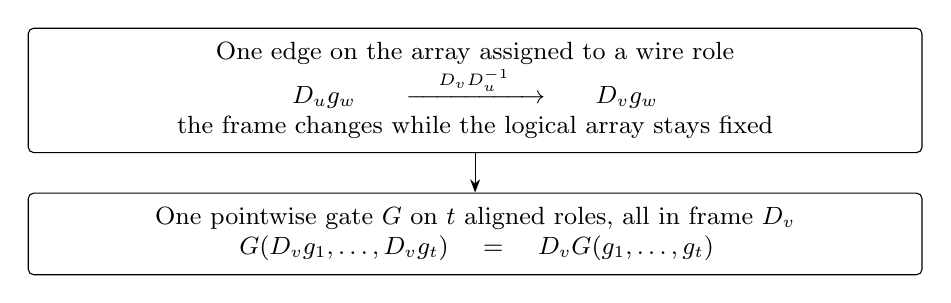
\begin{tikzpicture}[node distance=5mm, every node/.style={font=\small}, box/.style={draw,rounded corners=2pt,align=center,text width=11cm,inner sep=5pt}, >=Stealth]
\node[box] (c) {One edge on the array assigned to a wire role\\
$D_u g_w\ \xrightarrow{\quad D_vD_u^{-1}\quad}\ D_v g_w$\\
the frame changes while the logical array stays fixed};
\node[box,below=of c] (d) {One pointwise gate $G$ on $t$ aligned roles, all in frame $D_v$\\
$G(D_vg_1,\ldots,D_vg_t)=D_vG(g_1,\ldots,g_t)$};
\draw[->] (c)--(d);
\end{tikzpicture}

\caption{An edge changes the representation of one role's logical array
$g_w$. At the next gate $G$, all $t$ input arrays have the common frame
$D_v$, so the pointwise linear gate commutes with that frame. The same
$D_v$ acts on each output component.}
\label{fig:frame-compatibility}
\end{figure}

\subsection{Subspaces attached to the gates}

The scalar network already has the required signed exchange. We now
choose its intermediate labels to make the changes of frame inexpensive.
A label is a nondegenerate subspace of a fixed bilinear space. On every
edge one label will contain the other. For such an edge, the
\emph{orthogonal residual} is the orthogonal complement of the smaller label inside
the larger one; its dimension is the absolute change in label dimension.
The saving will come from keeping the total dimension lost on decreasing
edges small relative to $N$.

For the bit network, let $F=\mathbb Q^h$ with bilinear form
\[
 \langle x,y\rangle=x^{\mathsf T}(I-J/9)y,
\]
where $J$ is the all-one matrix.  This form has eigenvalues $1$ and
$1-h/9=-91/9$, so it is nondegenerate.  For a triple $T$ let $t_T$ be
its indicator vector.  Then
\[
 \langle t_S,t_T\rangle=|S\cap T|-1,
 \qquad \langle t_T,t_T\rangle=2.
\]
For the complex network, take instead $F=\mathbb F_2^h$ with the
ordinary dot product; here $t_T\cdot t_T=1$.
Thus every triple line is nondegenerate, and neighboring triple lines
are orthogonal, in the label field belonging to either construction.
The scalar domain need not equal the label field.
These degree-one intersection formulas specialize the construction
described by Alon~\cite[Section~3, remark after Theorem~1.1]{Alon1998}
to the prime $2$, with the ground-set size changed to $h=100$.

The ambient label space is $\mathcal F=F^{\otimes3}$ with its tensor
bilinear form.  It has dimension $m$ and is nondegenerate.  Write
\[
 u_a=t_{a_1}\otimes t_{a_2}\otimes t_{a_3},\qquad U_a=\langle u_a\rangle.
\]
The prescribed terminal labels are
\[
\begin{array}{c|cc}
\text{role}&\text{source label}&\text{sink label}\\ \hline
X_a&U_a&\mathcal F\\
Y_a&0&U_a^\perp\\
\text{each scratch role}&0&\mathcal F.
\end{array}
\]
Write $W$ for the wire count in the construction under consideration.
The source dimensions sum to $N$ and the sink dimensions to $Wm-N$.
Thus the signed dimension changes will sum to $Wm-2N$, because the
contributions at gates cancel. If decreasing edges lose a total
dimension $L$, the sum of absolute changes is $Wm-2N+2L$.
We will obtain $L<N/2$. The rational interface below will require
an additional $N$ source ranks, so this inequality will leave a strict
saving in both constructions.

At stage $j$, fix an invocation.  Put
\[
 A=F^{\otimes(j-1)},\qquad
 P=\langle t_{a_1}\otimes\cdots\otimes t_{a_{j-1}}\rangle,
 \qquad B=P^\perp\subset A.
\]
An empty tensor product is the one-dimensional ground field; thus
$B=0$ at stage 1.  Let
$Q=\langle t_{a_{j+1}}\otimes\cdots\otimes t_{a_3}\rangle
\subset F^{\otimes(3-j)}$, again using the empty tensor product at
stage 3.  Since $P$ is nondegenerate,
$A=B\mathbin{\perp}P$.  
We prescribe the following transition for each data wire in the stage,
where $t$ is the indicator of that wire's $j$th triple:
\[
\begin{array}{c|c|c}
 &\text{incoming label}&\text{outgoing label}\\ \hline
 X&A\otimes\langle t\rangle\otimes Q&(A\otimes F)\otimes Q\\
 Y&B\otimes\langle t\rangle\otimes Q&
 \bigl((B\otimes F)\mathbin{\perp}(P\otimes t^\perp)\bigr)\otimes Q.
\end{array}
\]
The outgoing $Y$ label can also be written
$(P\otimes\langle t\rangle)^\perp_{A\otimes F}\otimes Q$.
These transitions expose one tensor factor at each stage. To see that
they fit together, for $j<3$ write
$Q=\langle t_{a_{j+1}}\rangle\otimes Q'$. The next stage has
\[
 A'=A\otimes F,\qquad
 P'=P\otimes\langle t\rangle,\qquad
 B'=(P')^\perp_{A'}
    =(B\otimes F)\mathbin{\perp}(P\otimes t^\perp).
\]
Thus the prescribed outgoing labels are
$A'\otimes\langle t_{a_{j+1}}\rangle\otimes Q'$ on $X$ and
$B'\otimes\langle t_{a_{j+1}}\rangle\otimes Q'$ on $Y$, exactly
the next incoming labels. At stage 1 they start at $U_a$ on $X_a$
and zero on $Y_a$; at stage 3 they end at $\mathcal F$ on $X_a$
and $U_a^\perp$ on $Y_a$, as prescribed at the terminals.

The gate labels are organized by the decomposition
\[
 A\otimes F=(B\otimes F)\mathbin{\perp}(P\otimes F),
\]
with the common summand $B\otimes F$ and the remaining summand
$P\otimes F$ of dimension $h$. Suppress the one-dimensional factor
$Q$ for the moment. On a side wire joining neighboring physical triples
with indicators $t_X,t_Y$, the common component grows to $B\otimes F$,
while the remaining component passes through
\[
 P\otimes\langle t_X\rangle
 \ \subset\ P\otimes t_Y^\perp
 \ \subset\ P\otimes F.
\]
The first inclusion is possible because $t_X\perp t_Y$.
For the central gates we assign $A\otimes F$ on the physical $X$
bank and $B\otimes F$ on the physical $Y$ bank. A central wire
returns once from the former label to the latter, losing exactly
$P\otimes F$. The gate order below confines all decreases to this
return, while the other edges realize the prescribed stage transitions.

Number the successive times in an invocation by
$r=0,\ldots,7$. At stages 1 and 3, time $r$ uses row $r$ of the scalar
schedule~\eqref{eq:motif-schedule}. At stage 2 it uses the inverse of
row $7-r$, with the logical banks exchanged. In either case the gates
touch the physical wires in the order
\[
 Y\text{-side},\quad Y\text{-center},\quad X\text{-side},\quad
 X\text{-center},\quad Y\text{-center},\quad Y\text{-side},\quad
 X\text{-center},\quad X\text{-side}.
\]
A side wire still joins neighboring physical triples in stage 2 because
the neighbor relation is symmetric. The following table assigns the
common gate labels. It suppresses the tensor factor $Q$; for a gate
indexed by a physical bank triple, $t$ denotes that triple's indicator.

\begin{equation}
\begin{array}{c|l|l}
\text{time}&\text{physical wires}&\text{common gate label}\\ \hline
0&Y,\ \text{its side wires}&B\otimes\langle t\rangle\\
1&Y,\ \text{all center wires}&B\otimes F\\
2&X,\ \text{its side wires}&(B\otimes F)\mathbin{\perp}(P\otimes\langle t\rangle)\\
3&X,\ \text{all center wires}&A\otimes F\\
4&Y,\ \text{all center wires}&B\otimes F\\
5&Y,\ \text{its side wires}&(B\otimes F)\mathbin{\perp}(P\otimes t^\perp)\\
6&X,\ \text{all center wires}&A\otimes F\\
7&X,\ \text{its side wires}&A\otimes F.
\end{array}
\label{eq:motif-labels}
\end{equation}
All labels are tensored by $Q$ and viewed as subspaces of $\mathcal F$.
Every displayed summand is nondegenerate.

All scratch sources have label zero and all scratch sinks have label
$\mathcal F$, as prescribed above. The next lemma verifies the stage
boundaries and all intervening edge changes, including these scratch
edges.

\begin{lemma}\label{lem:motif-residuals}
Every edge joins comparable nondegenerate labels.  The only decreasing
edges are the central-wire edges from time 3 to time 4; their dimension
loss is $h$.  Consequently, if $c$ is the number of central wires per
invocation and $W$ the total number of wires, then
\begin{equation}
 L=Ich,\qquad
 \sum_{e}\bigl|\dim U_{\mathrm{head}(e)}-
                       \dim U_{\mathrm{tail}(e)}\bigr|
 =Wm-2N+2L.                                      \label{eq:rank-budget-labels}
\end{equation}
For the binary label space, every nonzero orthogonal residual of an
edge has an orthonormal basis.
\end{lemma}

\begin{proof}
Write $a=\dim A=h^{j-1}$ and $f=h^{3-j}$.  In the table below,
$\mathrm{in}$ denotes the preceding vertex on that data wire: its source
at stage 1, and its last gate in the preceding stage otherwise.  The
interstage calculation above gives its label.  The table lists the
orthogonal residual and its dimension for every edge except the final
data edges to their sinks, whose labels agree and whose residuals are zero.
Tensor each residual by $Q$, except in the last row.  The symbols $t_X,t_Y$ are
the indicators of the neighboring physical triples joined by a side wire.
\[
\begin{array}{l|l|r}
\text{wire and edge}&\text{orthogonal residual}&\text{dimension}\\ \hline
X:\ \mathrm{in}\to2&B\otimes t_X^\perp&(a-1)(h-1)\\
X:\ 2\to3&P\otimes t_X^\perp&h-1\\
X:\ 3\to6,\ 6\to7&0&0\\
Y:\ \mathrm{in}\to0&0&0\\
Y:\ 0\to1&B\otimes t_Y^\perp&(a-1)(h-1)\\
Y:\ 1\to4&0&0\\
Y:\ 4\to5&P\otimes t_Y^\perp&h-1\\
\mathrm{center}:\ \mathrm{source}\to1&B\otimes F&(a-1)h\\
\mathrm{center}:\ 1\to3&P\otimes F&h\\
\mathrm{center}:\ 3\to4&P\otimes F&h\\
\mathrm{center}:\ 4\to6&P\otimes F&h\\
\mathrm{side}:\ \mathrm{source}\to0&B\otimes\langle t_Y\rangle&a-1\\
\mathrm{side}:\ 0\to2&(B\otimes t_Y^\perp)\mathbin{\perp}(P\otimes\langle t_X\rangle)
 &(a-1)(h-1)+1\\
\mathrm{side}:\ 2\to5&P\otimes\langle t_X,t_Y\rangle^\perp&h-2\\
\mathrm{side}:\ 5\to7&P\otimes\langle t_Y\rangle&1\\
\mathrm{scratch}:\ \mathrm{last}\to\mathrm{sink}
 &(A\otimes F)\otimes Q^\perp&ah(f-1).
\end{array}
\]
The last gate on a central wire is at time 6, and the last gate on a side
wire is at time 7.  Both have label $(A\otimes F)\otimes Q$.  Enlarging it
to $\mathcal F$ at the sink gives the last residual in the table, with
$Q^\perp$ taken in the entire future tensor space.
The side edge $2\to5$ uses the neighbor relation
essentially.  Since $t_X\perp t_Y$, we have
$\langle t_X\rangle\subset t_Y^\perp$.  Hence its two labels satisfy
\[
 (B\otimes F)\mathbin{\perp}(P\otimes\langle t_X\rangle)
 \ \subset\
 (B\otimes F)\mathbin{\perp}(P\otimes t_Y^\perp).
\]
The complement of $\langle t_X\rangle$ inside $t_Y^\perp$ is
$\langle t_X,t_Y\rangle^\perp$, of dimension $h-2$; tensoring by
$P$ and then by $Q$ gives the residual in the table.  The other entries
follow directly by splitting $A=B\mathbin{\perp}P$ and
$F=\langle t\rangle\mathbin{\perp}t^\perp$.
Label dimension is nondecreasing along every edge except center $3\to4$, which removes
$P\otimes F\otimes Q$.  The table includes the interstage edges through
$\mathrm{in}$, and the initial and final data labels match their terminals,
so no other dimension changes occur.

The signed sum of dimension changes telescopes at every gate: each
touched wire has one incoming and one outgoing incidence with the same
gate label.  The sum of source dimensions is $N$, while the sum of
sink dimensions is $Wm-N$.  The signed increase is therefore $Wm-2N$.
There are $Ic$ decreasing edges, each of loss $h$; replacing signed
changes by absolute changes adds $2L$.

Now work over $\mathbb F_2$.  A nondegenerate symmetric bilinear space
is nonalternating precisely when it contains a vector of norm one.
The lines $P,Q$ have such vectors.  If $B\ne0$, a coordinate unit
outside the support of the earlier tensor vector belongs to $B$:
that support has size $3^{j-1}<h^{j-1}$ when $j>1$.
The same argument gives a unit vector in $Q^\perp$ when it is nonzero.
A triple complement, and the complement of two neighboring triple
lines, contain coordinate units outside supports of sizes at most
three and six, respectively.  Full tensor spaces contain coordinate
units as well.  In each nonzero tensor summand, tensoring these chosen
norm-one vectors gives a norm-one vector; placing it in that orthogonal
summand gives one in the whole residual.  Each residual is nondegenerate
by the decompositions above.  Thus every nonzero residual is nonalternating.

For completeness, every nondegenerate nonalternating binary symmetric
space has an orthonormal basis.  Split off unit lines until the
remaining space is alternating.  A nonzero nondegenerate alternating
space splits into planes with bases $a,b$ satisfying
$a\cdot a=b\cdot b=0$, $a\cdot b=1$; this follows by choosing a
nonzero $a$, choosing $b$ with $a\cdot b=1$, and taking the orthogonal
complement of their nondegenerate plane.  Retain one unit vector $w$
from the lines already split off.  A plane orthogonal to $w$ can be
absorbed into that line: the three vectors
\[
 w+a,\qquad w+b,\qquad w+a+b
\]
are independent, pairwise orthogonal, and have norm one.
Use one of these new unit vectors in place of $w$ for the next plane;
the remaining planes are still orthogonal to it.  Repeating this
operation absorbs every alternating plane.
\end{proof}

The loss ratios have the exact values
\[
 \frac{L_{\rm b}}{N}=\frac{100}{539},\qquad
 \frac{L_{\rm c}}{N}=\frac{101}{539}.
\]
In particular, both are smaller than $1/2$.  We now turn the dimension
count into the two interfaces needed later.

\subsection{The rational matrix interface}

For a nondegenerate rational subspace $U\subset\mathcal F$, write
$P_U$ for the projection onto $U$ along $U^\perp$.  Assign $P_U$ to
each gate or sink with label $U$.  Assign the source matrix $-P_{U_a}$
to $X_a$ and zero to every other source.
These are fixed rational $m\times m$ matrices; write $M_v$ for the matrix
at vertex $v$.  Define
$\rho(X_a)=Y_a$, $\rho(Y_a)=X_a$, and let $\rho$ fix every auxiliary
wire.

In the tape application, two address chunks are written as vectors $H,D$
of $m$ fields.  For a matrix $M$, the frame $\Phi_M$ moves the array entry
at $(H,D)$ to $(H+MD,D)$, leaving the other address fields unchanged.
The fields use a radix coprime to the fixed denominators, and addition is
modulo their common range.  Hence $\Phi_M$ is an invertible
$\mathbb F_2$-linear permutation of array entries, and
$\Phi_{M'}\Phi_M=\Phi_{M'+M}$.  Using $D_v=\Phi_{M_v}$
in \eqref{eq:common-frame-identity}, the endpoint matrix difference on each
routed role is exactly the shear applied to that role.  The following identity
makes it the same shear $H\gets H+D$ on every role;
Section~\ref{sec:tape-interchange} turns that shear into a field interchange
and implements an edge change with one smaller interchange per unit of its
rational rank.

\begin{proposition}\label{prop:bit-motif-interface}
The bit network has $W_{\rm b}$ wires, uses only pointwise XOR gates,
and sends its input vector to the permutation $\rho$ of that vector.
Its rational matrices are common to all incidences of a gate and obey
\[
 M_{\mathrm{sink}(\rho(w))}-M_{\mathrm{source}(w)}=I_m
 \quad\text{for every input role }w.
\]
The sum of the rational ranks of all edge differences is
\begin{align}
 s_{\rm b}
 &=\sum_{e}\operatorname{rank}_{\mathbb Q}
      (M_{\mathrm{head}(e)}-M_{\mathrm{tail}(e)})\\
 &=W_{\rm b}m-N+2L_{\rm b}
  =177176569088785861287000000<W_{\rm b}m.
\end{align}
\end{proposition}

\begin{proof}
Lemma~\ref{lem:scalar-motifs} gives the scalar permutation, including
all auxiliary roles.  For $U\subset V$ nondegenerate,
$P_V-P_U$ is the identity on $V\cap U^\perp$ and zero on its
orthogonal complement.  Its rank is $\dim V-\dim U$; reversing the
edge negates the matrix without changing its rank.
The only exceptions are the $N$ negative source projections.
At stage 1, $B=0$, and the first gate on $X_a$ has label exactly $U_a$.
Its first edge matrix is therefore $2P_{U_a}$, of rational rank one,
where the corresponding dimension change was zero.
Lemma~\ref{lem:motif-residuals} consequently gives the stated rank sum.
Its deficit from $W_{\rm b}m$ is $N-2L_{\rm b}>0$.

For an input $X_a$ the endpoint difference is
$P_{U_a^\perp}-(-P_{U_a})=I_m$.  Every other role has zero source
matrix and identity sink matrix.  This proves the interface.
\end{proof}

\subsection{The binary phase interface}

Use the complex scalar network and binary labels.  For a binary vector
$x$, let $\operatorname{wt}(x)$ denote its integer Hamming weight, and
write $[b]\in\{0,1\}$ for the integer representative of $b\in\mathbb F_2$.
For a label $U$, let
\[
 q_U(x)=\operatorname{wt}(P_Ux)\pmod4.
\]
The projection here is over $\mathbb F_2$.
Let
\[
 H=\frac1{\sqrt2}\begin{pmatrix}1&1\\1&-1\end{pmatrix},\quad
 C=H\begin{pmatrix}1&0\\0&i\end{pmatrix}H
   =aI+bX,\qquad a=\frac{1+i}{2},\quad b=\frac{1-i}{2},
\]
where $X$ interchanges the two coordinates.  On functions of
$x\in\mathbb F_2^m$ define
\[
 \mathcal C_U=H^{\otimes m}\operatorname{diag}_x(i^{q_U(x)})H^{\otimes m}.
\]
The use of $H$ in this definition is an identity of matrices.  Each entry
of $\mathcal C_U$ and its inverse is a Gaussian integer divided by $2^m$,
so both preserve arrays over $\mathbb Z[i,1/2]$.  The kernels implemented
below have Gaussian dyadic coefficients.

To apply the scalar network to these functions, replace the scalar on
each wire $w$ by an array
$f_w:\mathbb F_2^m\to\mathbb Z[i,1/2]$.  At each address, a gate
applies its scalar linear map to the values on the wires it touches.
The frame in \eqref{eq:common-frame-identity} is $D_v=\mathcal C_U$ at a
vertex with label $U$.  On an edge from label $U$ to label $V$, apply
$\mathcal C_V\mathcal C_U^{-1}$ to that wire's array.
All frames are diagonalized by the same matrix $H^{\otimes m}$.
For an integer $k\ge1$, an address for $k$ columns is
$(x^{(1)},\ldots,x^{(k)})\in(\mathbb F_2^m)^k$; every frame and edge
operator is then the tensor product of its one-column version over
these $k$ coordinates.  Each scalar gate is still applied once at each
joint address, to the vector of values on the roles it touches.

\begin{proposition}\label{prop:complex-motif-interface}
For each edge of the complex network, write $U,V$ for its tail and
head labels.  Its phase-frame difference
$\mathcal C_V\mathcal C_U^{-1}$ is a product of one translation
kernel $aI+bX_v$, or its inverse, per vector in an orthonormal basis
of the edge residual.  Here $(X_vf)(x)=f(x+v)$.
The sum of these basis lengths is
\[
 s_{\rm c}=W_{\rm c}m-2N+2L_{\rm c}
 =1873807244636671267308000000<W_{\rm c}m.
\]
After source and sink diagonal corrections, and undoing the signed
bank exchange, telescoping these phase frames gives $C^{\otimes m}$
on every role, including auxiliary roles.  The same assertion holds
on any positive number of columns by taking tensor products over columns.
\end{proposition}

\begin{proof}
For binary vectors $z,w$,
\[
 \operatorname{wt}(z+w)
 =\operatorname{wt}(z)+\operatorname{wt}(w)
       -2|\operatorname{supp}(z)\cap\operatorname{supp}(w)|.
\]
If $z\cdot w=0$, the intersection cardinality is even, so weight is
additive modulo four.  If $V=U\mathbin{\perp}E$ and $\mathcal B$
is an orthonormal basis of $E$, it follows that
\[
 q_V(x)-q_U(x)=\sum_{v\in\mathcal B}
                 \operatorname{wt}(v)[v\cdot x]\pmod4.
\]
For a decreasing edge the right side is negated.
Each $v$ has norm one, so $\operatorname{wt}(v)$ is odd.  Its
coefficient in the phase, including the sign for the edge direction,
is therefore some $\varepsilon\in\{1,-1\}$ modulo four.  The function
$i^{\varepsilon[v\cdot x]}$ equals
\[
 \frac{1+i^\varepsilon}{2}
 +\frac{1-i^\varepsilon}{2}(-1)^{v\cdot x}.
\]
The identity $H\operatorname{diag}(1,-1)H=X$, tensored over the
coordinates in $\operatorname{supp}(v)$, sends the diagonal character
$(-1)^{v\cdot x}$ to translation $X_v$.  The displayed phase therefore
becomes $aI+bX_v$ or its inverse.  The nonzero residuals have such
bases by Lemma~\ref{lem:motif-residuals}; for a zero residual use the
empty basis.  The same lemma gives the count $s_{\rm c}$.
The deficit is $2N-2L_{\rm c}>0$.

For an edge $e$, write $\mathcal B_e$ for its residual basis and
$K_{e,v}$ for the forward or inverse translation kernel associated
with $v\in\mathcal B_e$.  Taking tensor products preserves their
product, so on $k$ columns
\[
 \bigl(\mathcal C_V\mathcal C_U^{-1}\bigr)^{\otimes k}
 =\prod_{v\in\mathcal B_e}K_{e,v}^{\otimes k}.
\]
Thus each residual vector contributes one factor acting on all $k$
columns, and there are $s_{\rm c}$ such factors over the network.

Let $\rho$ denote the underlying permutation of the complex roles: it
exchanges $X_a,Y_a$ and fixes each scratch role.
By Lemma~\ref{lem:scalar-motifs}, the pointwise scalar network sends an input array at
$X_a$ to $Y_a$ with sign $+1$, an input at $Y_a$ to $X_a$ with sign
$-1$, and each scratch input to its own output with sign $+1$.
Applying \eqref{eq:common-frame-identity} with $D_v=\mathcal C_{U_v}$,
where $U_v$ is the label at vertex $v$, shows that an input role $w$ reaches
output role $\rho(w)$ with that sign and with operator
$\mathcal C_{U_{\mathrm{sink}(\rho(w))}}
 \mathcal C_{U_{\mathrm{source}(w)}}^{-1}$.
For $k$ columns, use $D_v=\mathcal C_{U_v}^{\otimes k}$ on the joint
address set in the same identity.  The route operator is then the $k$th
tensor power of the displayed address operator, multiplied by its scalar
route sign once.
The zero label has frame $I$, while the full label has frame
$C^{\otimes m}$ because $q_{\mathcal F}(x)=\operatorname{wt}(x)$.
Every pair except $X_a\to Y_a$ has these zero and full labels.
For the remaining pair, write $u=u_a$.  Its binary norm is one and
its weight is $3^3=27$.  Orthogonal weight additivity yields
\begin{align*}
 q_{U_a^\perp}(x)-q_{U_a}(x)
 &=\operatorname{wt}(x)-2\operatorname{wt}(u)[u\cdot x]\\
 &=\operatorname{wt}(x)+2[u\cdot x]\pmod4.
\end{align*}
Since $2[u\cdot x]\equiv2\sum_{j\in\operatorname{supp}(u)}x_j
\pmod4$, the operator on $X_a\to Y_a$ is the tensor of $C^{-1}$ on the
27 coordinates of $\operatorname{supp}(u)$ and $C$ elsewhere.
Put $Z=\operatorname{diag}(1,-1)$.  Direct multiplication gives
\[
 C=iZC^{-1}Z,\qquad C^{-1}=-iZCZ.
\]
For $k$ columns, let $Z_{a,k}$ be the tensor product of $Z$ on
those 27 coordinates in every column and the identity elsewhere.
Apply $Z_{a,k}$ before the network at $X_a$, and apply
$i^{27k}Z_{a,k}$ after the network at $Y_a$; the latter scalar is
applied once to the whole role.  There are $27k$ inverse factors, so
the identity $C=iZC^{-1}Z$ turns each of them into $C$.  The operator
on this pair is therefore $C^{\otimes mk}$ as well.
Only the physical $X$ outputs still carry the minus sign of the
scalar exchange.  Negate those outputs and send output role $\rho(w)$
back to role $w$.  Every role, including every scratch role, now has
the required forward tensor product.
\end{proof}

\subsection{Explicit rational bounds for the two recurrences}

The relative rank deficits are
\[
 \eta_{\rm b}=\frac{W_{\rm b}m-s_{\rm b}}{W_{\rm b}m}
       =\frac{339}{22587335000000},\qquad
 \eta_{\rm c}=\frac{W_{\rm c}m-s_{\rm c}}{W_{\rm c}m}
       =\frac{73}{19906842167500}.
\]
For both recurrences we may use the fixed rational exponent
\begin{equation}
 \tau=\sigma=1-2^{-50}.
 \label{eq:explicit-motif-exponents}
\end{equation}
Both exact deficits displayed above are greater than $20\cdot2^{-50}$.
Since $m<2^{20}$ and $\log 2<1$, we have $\log m<20$, whence
\[
 m^{1-2^{-50}}
 =m\exp(-2^{-50}\log m)
 >m(1-20\cdot2^{-50})>m(1-\eta)
\]
for either $\eta=\eta_{\rm b}$ or $\eta=\eta_{\rm c}$.
Consequently
\[
 \frac{s_{\rm b}}{W_{\rm b}}<m^\tau,
 \qquad \frac{s_{\rm c}}{W_{\rm c}}<m^\sigma,
 \qquad 0<\tau=\sigma<1.
\]
Here $\sigma$ is a rational upper bound for the logarithmic exponent
of the complex recurrence.

\section{Faster interchange of address chunks}
\label{sec:tape-interchange}

We use the bit network to interchange two equal address chunks on tape.
An edge matrix of rank $a$ will require $a$ smaller interchanges.
Because the sum of these ranks is less than the number of wires times
$m$, the resulting recurrence saves a power of the chunk width.

\subsection{A matrix decomposition adapted to tape order}

Lemma~\ref{lem:ordered-affine-streams} updates a later field using
earlier fields in linear time.  Lower triangular changes of coordinates
can be performed entirely in this direction. The required factorization
is the Bruhat factorization for arbitrary matrices, with coordinate order
reversed; see Grigor'ev~\cite[Appendix~A.2, Proposition~14(c)]{Grigoriev1982}.
We give its elementary elimination proof in this order.

\begin{lemma}[Lower triangular factorization]
\label{lem:lower-lower}
Every rational $m\times m$ matrix $A$ of rank $a$ has a factorization
\[
 A=E_1\Pi E_2,
\]
where $E_1,E_2$ are invertible lower triangular rational matrices and
$\Pi$ has exactly $a$ entries equal to one, with at most one in each row
and column, and all remaining entries zero.
\end{lemma}

\begin{proof}
If $A=0$, take $E_1=E_2=I$ and $\Pi=0$.  Otherwise choose the topmost
nonzero row and its rightmost nonzero entry.  Use that pivot column to
clear entries to its left by right multiplication by lower triangular
elementary matrices.  There are no nonzero entries to its right in the
pivot row.  Clear entries below the pivot by left multiplication by
lower triangular elementary matrices, and scale the pivot to one.
All rows above the chosen row were zero in the still active columns.

Delete the pivot row and column from the active index sets, retaining
their original orders, and repeat.  Elementary operations on the active
indices are still lower triangular in the original order.  They do not
change any earlier pivot row or column, whose other entries have already
been cleared.  Each step isolates a rank-one block and leaves the
remaining rank in the active submatrix.  Thus the final partial
permutation matrix has exactly $a$ ones.  If $LAR=\Pi$ is the resulting
identity, then $E_1=L^{-1}$ and $E_2=R^{-1}$ have the required form.
\end{proof}

\begin{lemma}[The cost of a rational matrix shear]
\label{lem:matrix-shear}
Let $\mathcal A$ be a fixed finite collection of rational $m\times m$
matrices.  There is a fixed odd prime $q$ such that the following holds.
Let $H=(H_1,\ldots,H_m)$ and $D=(D_1,\ldots,D_m)$ be two ordered
groups of fields, every field ranging over $[q^b]$, with every $H_i$
before every $D_j$.  For $A\in\mathcal A$ of rational rank $a$, the
permutation
\[
 (H,D)\longmapsto(H+AD,D)
 \quad\text{over }\mathbb Z/q^b\mathbb Z
\]
can be performed with exactly $a$ interchanges of pairs of $b$-digit
fields and $O(V)$ further work.  Every interchange is between an $H$
field and a $D$ field.  Spectators between any of the formal fields are
allowed.
\end{lemma}

\begin{proof}
Choose the factorizations of Lemma~\ref{lem:lower-lower} for all matrices
in $\mathcal A$ once and for all.  Include their factors and inverses in
a finite rational table.  Choose an odd prime avoiding every denominator
in the table and every numerator of a diagonal entry of an invertible
factor.  For example, a prime exceeding the absolute values of all its
nonzero numerators and denominators suffices.  Rational elimination and
trial division construct this finite table and a suitable prime in a
finite computation independent of $b$.  They may therefore be compiled
into one fixed machine description.  All these
rational identities then specialize to $\mathbb Z/q^b\mathbb Z$, and
the triangular factors remain invertible there.

A lower triangular transformation of $H$, or of $D$, costs $O(V)$:
update coordinates in descending physical order.  At coordinate $i$,
multiply by its diagonal unit and add a fixed linear combination of
earlier coordinates.  These earlier coordinates still have their original
values.  Apply Lemma~\ref{lem:ordered-affine-streams}; the number of
coordinates is the fixed number $m$.  Inverses are also lower triangular.

For $A=E_1\Pi E_2$, first transform $D$ by $E_2$ and $H$ by $E_1^{-1}$,
then add $\Pi D$ to $H$, and finally transform $H$ by $E_1$ and $D$ by
$E_2^{-1}$.  Each one in position $(i,j)$ of $\Pi$ calls for
$H_i\leftarrow H_i+D_j$.  Implement it by
\[
 D_j\leftarrow D_j+H_i,\qquad
 (H_i,D_j)\leftarrow(D_j,H_i),\qquad
 D_j\leftarrow H_i-D_j.
\]
The first and last updates target a later field controlled by an earlier
field.  On an initial pair $(h,d)$ this sequence yields $(h+d,d)$.
It uses just one interchange.  There are $a$ ones, which proves the
claim.  In particular, the number of recursive calls is the rational
rank $a$; temporary tapes used for the other operations do not multiply
that count.
\end{proof}

\subsection{Transferring a finite circuit to address permutations}

Fix integers $m,W\ge2$.  The circuit has $W$ wires, including its
scratch wires, with separate input and output terminals.  Its fixed,
pointwise bit gates induce a permutation $\rho$ of the $W$ scalar inputs
at completion: the input value at role $w$ appears at output role
$\rho(w)$.  Assign a
rational $m\times m$ matrix to each terminal and to each gate, the latter
assignment being common to every wire at that gate.  A wire segment
between consecutive assigned vertices is called an edge.  For an edge
$e$ put
\[
 A_e=M_{\mathrm{head}(e)}-M_{\mathrm{tail}(e)},
 \qquad s=\sum_e\operatorname{rank}_{\mathbb Q}A_e.
\]
The required conditions are
\begin{equation}
\label{eq:finite-shear-contract}
 M_{\mathrm{out}(\rho(w))}-M_{\mathrm{in}(w)}=I_m
 \quad(1\le w\le W),\qquad s<Wm.
\end{equation}
All these data are finite and fixed. Proposition~\ref{prop:bit-motif-interface}
supplies these conditions with $W=W_{\rm b}$ and $s=s_{\rm b}$.
Its negative source projection is essential to the endpoint identity and
has already been included in the rank sum.

\begin{proposition}[Power-width interchange with rows]
\label{prop:power-interchange}
Assume the fixed circuit data satisfy
\eqref{eq:finite-shear-contract}, and let $q$ be a prime as in
Lemma~\ref{lem:matrix-shear} for its edge matrices, also avoiding the
denominators of every assigned terminal and gate matrix $M$.
Choose a rational number $\tau\in(0,1)$ with $s/W<m^\tau$.
For every $e=m^k$, $k\ge0$, consider two disjoint contiguous address
chunks of $e$ radix-$q$ digits each.  Suppose a row field preceding both
chunks has length divisible by $W^k$.  There may be additional fields
before and after the row field, between the chunks, and after them.
The chunks can be interchanged in $O(Ve^\tau)$ time, preserving every
other address field, on a fixed number of finite-alphabet tapes.
The constant is independent of all field lengths and of the data.
\end{proposition}

\begin{proof}
For $k=0$ apply the single-digit operation of
Lemma~\ref{lem:elementary-streams}.  For $k>0$, write each chunk as $m$
consecutive $b=e/m$ digit fields, giving vectors $H,D$ over
$\mathbb Z/q^b\mathbb Z$.  We first construct the shear $H\leftarrow H+D$.

Split whole rows cyclically into $W$ role streams within each prefix
preceding the row field.  Write the original row number as
$r=Wg+(w-1)$ with $1\le w\le W$; stream $w$ has row number $g$.
These streams have exactly the same remaining shape, including the
full ranges of $H$ and $D$.  Each has
logical volume $V/W$, and its row count is divisible by $W^{k-1}$.

For a rational matrix $M$, let $\Phi_M$ act on an array by moving its
entry at address $(H,D)$ to $(H+MD,D)$, with every spectator unchanged.
Thus $\Phi_M$ is the array permutation induced by that address map.
Its inverse is $\Phi_{-M}$ and
$\Phi_{M'}\Phi_M=\Phi_{M'+M}$.  On every circuit edge apply
$\Phi_{A_e}$ to that role stream; implement it by
Lemma~\ref{lem:matrix-shear}, recursively interchanging each pivot pair
of $b$-digit fields.  Execute each circuit gate pointwise at matching
addresses of its role streams.

The row split supplies the common address set used in the
frame identity~\eqref{eq:common-frame-identity}. Here the frame at a
vertex with matrix $M$ is the address permutation $\Phi_M$, and every
edge changes it by $\Phi_{M'-M}$. The same invariant proof applies
because a common address permutation commutes with every pointwise
bit gate. For the physical input arrays $f_w$, the logical arrays are
$g_w=\Phi_{-M_{\mathrm{in}(w)}}f_w$; this only specifies their
interpretation, with no initial tape operation. The logical circuit
routes $g_w$ to role $\rho(w)$. Thus its physical output satisfies
\[
 f'_{\rho(w)}
 =\Phi_{M_{\mathrm{out}(\rho(w))}}
   \Phi_{-M_{\mathrm{in}(w)}}f_w
 =\Phi_{I_m}f_w,
\]
by~\eqref{eq:finite-shear-contract}. Merge by returning row $g$ of
output role $\rho(w)$ to the original row $Wg+(w-1)$ within the same
preceding prefix. This undoes $\rho$ and restores row order. The result
is $H\leftarrow H+D$ on every original row, including rows assigned
to scratch roles, whose initial values were arbitrary.

To interchange the two full chunks, perform
\[
 D\leftarrow D-H,\qquad H\leftarrow H+D,\qquad D\leftarrow H-D,
\]
componentwise.  Only the middle shear uses the circuit.  The other two
updates target the later group and have linear cost.  The transformation
sends $(H,D)$ to $(D,H)$.

The number of recursive calls is the sum of the edge ranks, exactly $s$.
Each acts on one role stream of volume $V/W$, retaining all other
fields as spectators.  Splitting,
merging, gates, and triangular operations have total cost $O(V)$ because
their number is fixed.  Below we verify that scheduling the recursive
calls on fixed tapes also costs $O(V)$ at this node.  Thus if $F_k$ is a
uniform upper bound for time divided by logical volume, then
\begin{equation}
\label{eq:swap-recurrence}
 F_0=O(1),\qquad F_k\le(s/W)F_{k-1}+O(1).
\end{equation}
For $a=s/W<m^\tau$ the geometric sum
$\sum_{j=0}^k a^j$ is $O(m^{k\tau})$.  If $a\le1$, the sum is at
most $k+1=O(m^{k\tau})$; if $a>1$, it is $O(a^k)$.
Hence $F_k=O(e^\tau)$.

\paragraph{A fixed-tape depth-first schedule.}
Here we complete the implementation assertion used in
\eqref{eq:swap-recurrence}.  Reserve $W$ role tapes, a fixed set of
I/O and elementary-operation work tapes, one parking stack tape, and a
separate descriptor stack.  Although $W$ is large, it is fixed.
At a call boundary all reusable work tapes, other than the current I/O
and local descriptor, are empty and their heads are at their origins.
The parking and descriptor heads are at the tops of their stacks.

Before a recursive call, append the $W-1$ inactive role streams to the
parking stack in a fixed order, with separators.  Copy the active stream
to the child I/O area, and erase the parent role tapes while traversing
their current contents.  Push the parent descriptor and its finite
program counter to the descriptor stack.  The role and work tapes are
now available to the child, using the same tapes at every depth.
On return, copy the child output into the designated active role.
Pop the inactive streams in reverse order.  To recover a stream in its
original direction, prepare its destination to the known length and
write the popped symbols from the destination's right end toward its
left end.  Erase the popped stack cells as they are left.  This uses
linear time and ends with the parking head at the previously saved top.
No scan passes through a parked ancestor.  Cleanup is always limited to
the region visited by the current call; a reused tape is not swept to
the largest position ever visited by an ancestor.

Each push, pop, copy, positioning operation, or erasure moves $O(V)$
symbols at a parent node.  There are only the fixed number $s$ of child
calls.  This gives precisely the additional $O(V)$ term claimed above,
even though each child itself has volume $V/W$.  Temporary storage is
therefore not substituted for logical volume in the factor $s/W$.

For completeness, descriptor processing also fits this term when the
payload is one bit.  Let $V_0$ be the volume at the root of one
power-width call with width $e_0=m^{k_0}$, and $V_j=V_0/W^j$ the volume
of any depth-$j$ child.  Here $j\le k_0=\log_m e_0$.  The root row
count is at least $W^{k_0}$, so at depth $j$ it is still at least one.
Both original chunk ranges remain present: digits outside the current
subchunks become spectators rather than being removed.  Hence
\[
 V_j\ge q^{2e_0},\qquad
 j\log W\le(\log_m e_0)\log W=O(e_0)=O(\log V_j).
\]
It follows that
$\log V_0=\log V_j+j\log W=O(\log(2V_j))$.
A local descriptor lists the row field, at most the current $m+m$
fields, and a fixed number of intervals formed from intervening
spectator fields.  Computing products of their lengths, subdividing
target fields, copying lengths, and storing the current instruction take
$(\log(2V_0))^{O(1)}=O(V_j)$ time at that child, since every fixed
power of $\log(2V_j)$ is $O(V_j)$.  Before descending,
construct the child's descriptor by retaining its two target fields and
combining each consecutive group of spectator fields into one interval.
The ancestor's subdivision need not remain active in the child.  Stack entries contain
finite instructions and binary integers, not new alphabet symbols.
These observations establish one finite machine for every recursion
depth and every choice of spectator lengths.

\end{proof}


We use the rational value $\tau=1-2^{-50}$ established in
\eqref{eq:explicit-motif-exponents}. Its verification uses fixed integer
comparisons and the displayed exponential inequality; it needs no
real-arithmetic oracle.


\subsection{Removing width and row restrictions}

We have proved the fast operation for power widths with enough rows.
Rows for a general array can be supplied by a few of its own high digits.
Their movement will cost less than the final bound.

\begin{lemma}[Arbitrary-width interchange]
\label{lem:chunk-swap}
There exist fixed $0<\tau<1$ and one fixed finite-alphabet multitape
procedure with the following property.  For positive integers $P,G,B$
and $u\ge1$, it transforms an arbitrary bit array on
\[
 [P]\times[2^u]\times[G]\times[2^u]\times[B]
\]
by the address permutation
\[
 (p,h,g,d,z)\longmapsto(p,d,g,h,z)
\]
in $O(Vu^\tau)$ steps, where $V=PG B\,2^{2u}$.
The integers specifying the shape are part of the input.  The time
includes their processing, all padding and unpadding, and fixed-tape
workspace cleanup.  In particular, $B=1$ is allowed.
\end{lemma}

\begin{proof}
First suppose the two ranges are $[q^e]$, where $q$ is the fixed prime
already chosen.  Set
\[
 k=\lceil\log_m e\rceil,\qquad
 \rho=\left\lceil\frac{k\log W}{2\log q}\right\rceil.
\]
For all sufficiently large $e$, $1\le\rho<e$ and $\rho=O(\log(2e))$.
Handle the bounded remaining set of widths by $e$ individual digit
interchanges; the constant in $O(Ve^\tau)$ absorbs their cost.

Write each chunk as its top $\rho$ digits followed by its remaining
digits, denoted $h^+,h^-$ and $d^+,d^-$, respectively.  Interchange
the corresponding high digits one pair at a time.  The high positions
now contain $d^+$ and $h^+$; move the digits of the latter, preserving
their order, into consecutive positions immediately after $d^+$.
Suppressing the prefix and suffix, the field orders during the construction are
\[
\begin{aligned}
 &(h^+,h^-,g,d^+,d^-),\\
 &(d^+,h^+,h^-,g,d^-)
       &&\text{after exchanging and joining the high parts},\\
 &(d^+,h^+,d^-,g,h^-)
       &&\text{after interchanging the remaining parts},\\
 &(d^+,d^-,g,h^+,h^-)
       &&\text{after separating the high parts again}.
\end{aligned}
\]
In the two middle orders, the first two fields form a row field of range
\[
 R=q^{2\rho}\ge W^k
\]
before both remaining chunks.  The joining moves preserve the order of
the remaining digits and the gap field.  Exchanging and joining the high
parts costs $O(V\rho)$ by
Lemma~\ref{lem:elementary-streams}.  Append zero rows, separately within
each preceding prefix, until the row count is
\[
 R'=W^k\left\lceil R/W^k\right\rceil<2R.
\]
This changes the row field's length; it need not remain a power of $q$
during the computation.  The padded logical volume is less than $2V$.

Write the remaining width in base $m$:
\[
 e-\rho=\sum_{j=0}^{k} a_jm^j,\qquad 0\le a_j<m.
\]
Partition each remaining chunk into corresponding consecutive pieces,
with $a_j$ pieces of width $m^j$.  Apply
Proposition~\ref{prop:power-interchange} to each corresponding pair.
All these calls use the same row field of length $R'$, which is divisible
by each required $W^j$.  At completion every call preserves its row
address, so it neither mixes genuine rows with padded rows nor depends
on the values used for padding.  The padded zero rows remain zero at
these completed-call boundaries.  The sum of the costs is bounded by
\[
 O(V)\sum_j a_jm^{j\tau}=O(Ve^\tau).
\]
The fixed bound $a_j<m$ and the inequality $m^k<me$ make this a
geometric sum of the stated order.  Scan away the padded rows, then
reverse only the moves that joined the high parts.  This is the last
transition in the field-order display: $h^+$ returns to the later
high position, while $d^+$ stays in the earlier one.  The final order
is therefore the required interchange of the two full chunks.  The
remaining movement cost $O(V\log(2e))$ is $O(Ve^\tau)$.
Computing the piece list and every new shape is polynomial in
$\log(2V)$ per piece.  There are at most
$(m-1)(k+1)=O(\log(2e))$ pieces; since $V\ge q^{2e}$, their total
descriptor cost is a fixed power of $\log(2V)$ and hence $O(V)$.
Each power-width call uses the fixed schedule proved above and leaves
its work tapes clean.

Finally, for binary chunks let $e$ be the least integer with
$q^e\ge2^u$.  Pad each of the two chunk ranges numerically from $[2^u]$
to $[q^e]$, putting zero in an entry if either chunk coordinate is
invalid.  The increase in volume is less than $q^2$, a fixed factor.
The padding is a nested scan through consecutive valid and invalid
intervals, with their lengths prepared from the shape.  It costs $O(V)$
with a constant depending on $q$.  Lexicographic radix-$q$ order of
$[q^e]$ is its numerical order, just as binary order of $[2^u]$ is its
numerical order.  Padding therefore preserves the order of the existing
entries without converting the digits of every address.
The completed interchange preserves the set on which both chunk
coordinates lie below $2^u$.  Scan away the other entries to recover the
desired binary array.  Since $e=O(u)$ for fixed $q$, the bound is
$O(Vu^\tau)$.
\end{proof}

The lemma permits arbitrary prefix, gap, and suffix lengths.  Thus every
later interchange of equal bit chunks is an instance of its stated
layout, after multiplying the irrelevant contiguous lengths.
For widths differing by one bit, choose the leading bit of the longer
chunk as the extra bit.  Suppress the outer prefix and suffix, and write
$g$ for the intervening address field.  If the first chunk is longer,
write it as $(h_0,H)$, so $H$ and the second chunk $D$ have equal width.
The physical orders are
\[
 (h_0,H,g,D)\longmapsto(h_0,D,g,H)
              \longmapsto(D,g,h_0,H).
\]
The first step interchanges $H,D$ by the lemma; the second moves the
single bit $h_0$ immediately before $H$.  If the second chunk is longer,
write it as $(d_0,D)$, with $H$ the first chunk.  Use
\[
 (H,g,d_0,D)\longmapsto(d_0,H,g,D)
              \longmapsto(d_0,D,g,H).
\]
Here the first step moves $d_0$ immediately before $H$, and the second
interchanges $H,D$.  In each case $g$ remains between the two full chunks
in the final order.  If $H,D$ are empty, the indicated equal-width
interchange is the identity.  Each case uses one single-bit move, costing
$O(V)$ by Lemma~\ref{lem:elementary-streams}, in addition to the
equal-width interchange.  No unrestricted array transpose is being used
in these operations.

\section{Fast simultaneous synthetic butterfly layers}
\label{sec:fast-butterfly-layers}

We now apply the complex network to a common butterfly layer on several
axes. The array has complete address set
\[
 [P]\times[2^K]^D\times[S],\qquad 1\le D\le d,
\]
with $P,S\ge1$, in lexicographic order. Its $D$ consecutive $K$-bit
chunks each select the bit at one common offset $0\le\rho<K$, counted
from the least significant
end. Each address carries a polynomial record with $r$ complex
coefficients, initially in the unit disk on the grid
$2^{-p}\mathbb Z[i]$, with $\Theta(p)$ bits per real or imaginary
component. The intended operation is the tensor product
of $H_0(u,v)=((u+v)/2,(u-v)/2)$ on the $D$ selected bits, acting
coefficientwise and preserving all other address fields.

The parameters will satisfy
\[
 d=\Theta(p^\epsilon),\qquad K=\lfloor d^c\rfloor,
 \qquad r=2^{\Theta(p/d)},\qquad c>0,\quad 0<\epsilon<1.
\]
The exponents and comparison constants are fixed, and we impose their
further restrictions in Proposition~\ref{prop:simultaneous-layer}.
Two consequences explain the layout. The polynomial length $r$ grows
faster than every fixed power of $p$, so a scan of a record pays for
polynomial work on its address. Also $K/\log p\to\infty$, which will
make the exceptional set in a packed change of address bits small enough
to repair by sorting. We will obtain cost $O(Vd^{\lambda'})$, with
$\lambda'<1$ and $V$ the logical bit volume, whereas separate butterfly
factors would require $D$ whole-array passes.

We first construct tensor products of the auxiliary two-point kernel
$C$ from Proposition~\ref{prop:complex-motif-interface}. Its phase
frames express a $C$ tensor product using smaller groups of
selected bits, separated by binary changes of basis. We implement those
changes by moving whole address chunks. Splitting complete rows among
the network's wire roles then reduces the volume of each recursive
call. Finally, we bound the intermediate dyadic values and convert the
completed $C$ layer to the normalized $H_0$ layer. The entire layer is
evaluated exactly before one final truncation.

\subsection{Phase frames for a simultaneous butterfly layer}
\label{subsec:phase-frames}

Hold the unselected address bits fixed and regard the stored complex
values on one wire role as a function of the selected bits.  The phase
identities below express an edge's residual operator as a product of
two-point kernels on selected directions.

Put
\[
 H_0=\frac12\begin{pmatrix}1&1\\1&-1\end{pmatrix},\qquad
 H=\sqrt2 H_0,\qquad \mathsf S=\operatorname{diag}(1,i),\qquad
 Z=\operatorname{diag}(1,-1).
\]
For the bit-flip matrix $X=\bigl(\begin{smallmatrix}0&1\\1&0\end{smallmatrix}\bigr)$,
define
\begin{equation}\label{eq:phase-C}
 C=H\mathsf SH=aI+bX,\qquad a=\frac{1+i}{2},\quad b=\frac{1-i}{2}.
\end{equation}
Direct multiplication gives
\begin{equation}\label{eq:phase-basic-identities}
 H_0=b\mathsf SC\mathsf S,\qquad C^2=X,\qquad C^4=I,\qquad
 C^{-1}=bI+aX=-iZCZ.
\end{equation}
In particular, $C=iZC^{-1}Z$.  These identities use only Gaussian dyadic
coefficients.  The Hadamard matrices in the definition of
$\mathcal C_U$ are used to prove identities; they need not be executed
by the machine.

Consider an edge from label $U_-$ to label $U_+$, and choose an
orthonormal basis $v_1,\ldots,v_{\rho_{\rm edge}}$ of its residual.
Proposition~\ref{prop:complex-motif-interface} gives the frame change
\[
 \mathcal C_{U_+}\mathcal C_{U_-}^{-1}
 =\prod_{j=1}^{\rho_{\rm edge}}(aI+bX_{v_j})^{\epsilon_j},
 \qquad \epsilon_j\in\{1,-1\}.
\]
Here $(X_vf)(x)=f(x+v)$, and we write $C_v=aI+bX_v$.
The number of directional kernels is precisely
$\rho_{\rm edge}$, including on decreasing edges. The next step puts those directions
into coordinate positions without performing a general transpose.

\paragraph{Implementing an arbitrary residual basis.}
For $M\in\operatorname{GL}(m,\mathbb F_2)$, let $\mathcal P_M$ be the
address permutation that moves the value at $x$ to $Mx$.  Thus
$(\mathcal P_Mf)(x)=f(M^{-1}x)$, and
\begin{equation}\label{eq:phase-conjugation}
 \mathcal P_MX_v\mathcal P_M^{-1}=X_{Mv}.
\end{equation}
Extend $v_1,\ldots,v_{\rho_{\rm edge}}$ to a basis of $\mathbb F_2^m$ and take these vectors as
the first $\rho_{\rm edge}$ columns of $M$.  The displayed edge identity
then becomes
\begin{equation}\label{eq:phase-edge-coordinate}
 \mathcal C_{U_+}\mathcal C_{U_-}^{-1}
 =\mathcal P_M\left(\prod_{j=1}^{\rho_{\rm edge}}C_{e_j}^{\epsilon_j}\right)
   \mathcal P_M^{-1},
\end{equation}
where $e_j$ is the $j$th standard basis vector.  The matrix $M$ need not
preserve the dot product: equation~\eqref{eq:phase-conjugation} only
uses its invertibility.

For the array layout used below, take a group of $e=mf$ consecutive
axis chunks and divide it into $m$ consecutive slots of $f$ chunks,
numbered in physical order.
Number the chunks within each slot by $j=0,\ldots,f-1$, starting at
its least significant end.  Write $x_{h,j}$ for the selected bit in
chunk $j$ of slot $h$, where $1\le h\le m$.  Column $j$ is the vector
$(x_{1,j},\ldots,x_{m,j})$.  A frame on this group is the tensor
product of the same phase frame
$\mathcal C_U$ of Proposition~\ref{prop:complex-motif-interface}
on these $f$ columns.

To implement \eqref{eq:phase-edge-coordinate} on the group, first apply
$\mathcal P_M^{-1}$ separately to each column.  For each
$1\le h\le\rho_{\rm edge}$, apply $(C^{\epsilon_h})^{\otimes f}$ to the
$f$ bits $x_{h,0},\ldots,x_{h,f-1}$.  This is one child operation
on the $f$ axes in slot $h$.  Finally apply $\mathcal P_M$ to every
column.  A negative directional kernel still requires only one
forward child, because
\begin{equation}\label{eq:phase-inverse-child}
 (C^{-1})^{\otimes f}
 =(-i)^f Z^{\otimes f}C^{\otimes f}Z^{\otimes f}.
\end{equation}
The rightmost phase is applied first.  All inverse wrappers are address
signs and constant fourth-root phases, so they add no recursive calls.

Gaussian elimination expresses any $M\in\operatorname{GL}(m,\mathbb F_2)$
as a product of at most $m(m-1)+3m$ elementary row additions: one clears
at most $m-1$ other entries per pivot, and each row swap is three row
additions.  Reversing the elimination gives the required product since
each row addition is an involution.  The number is a constant because
$m$ is fixed.  Adding row $h'$ to row $h$ in every column applies
$x_{h,j}\leftarrow x_{h,j}\mathbin\oplus x_{h',j}$ for every
$0\le j<f$.  Thus one row addition changes corresponding selected
positions in two whole slots.  The packed address operation proved
below performs all of these XORs together.

\paragraph{The exact recursive contract.}
Apply the finite network with these column frames to a group of
$e=mf$ selected axes.  Summing its residual dimensions gives exactly
$s_{\rm c}$ child calls, each on the $f=e/m$ axes of one slot.
The source and sink $Z_{a,f}$ signs, together with the scalar
$i^{27f}$ at each affected sink, turn every endpoint kernel into a
forward one.  Negating the prescribed physical bank
and undoing its exchange returns each result to its original role.
Proposition~\ref{prop:complex-motif-interface} therefore gives
$C^{\otimes e}$ on every role, including roles whose initial scratch
values were arbitrary.  Formula~\eqref{eq:phase-inverse-child} supplies
each inverse child from one forward call, and none of the corrections
adds a child.  The remaining operations are a fixed number of binary
row additions and coefficientwise scalar operations.

\paragraph{Returning to normalized butterflies.}
For an address $x$ in a full layer, write $x_1,\ldots,x_D$ for its
selected bits.
The diagonal operator $\mathcal S_D$ multiplies the value stored at
an address by the phase determined by those bits:
\[
 (\mathcal S_D z)(x)=i^{x_1+\cdots+x_D}z(x).
\]
Here the unselected address bits are unchanged, and the same phase is
applied to every coefficient stored at that address.  Applying
\eqref{eq:phase-basic-identities} on all selected coordinates gives
\begin{equation}\label{eq:phase-butterfly-layer}
 H_0^{\otimes D}=b^D\mathcal S_D C^{\otimes D}\mathcal S_D.
\end{equation}
The scalar is
\[
 b^D=(-i/2)^{\lfloor D/2\rfloor}b^{D\bmod2},
\]
so it is a binary shift and fourth-root phase, with at most one further
factor $b$.  All phases, inverse wrappers, and scalar corrections above
are exact Gaussian dyadic operations.  Thus, once the physical binary
basis changes and recursive stream layout are supplied, the complete
parallel butterfly layer is exact up to its prescribed final truncation.

\subsection{Packed changes of selected address bits}
\label{sec:packed-selected-bits}

We implement a binary row addition on corresponding selected bits in two
address chunks. A third chunk supplies temporary address bits; its arbitrary
initial value must be restored. The construction first uses a constant number
of cyclic shifts of whole chunk ranges, then corrects an explicitly bounded set of
addresses. The correction depends only on addresses, so the time bound is
worst-case over all payloads.

We use three previously established streaming operations.
Lemma~\ref{lem:chunk-swap} exchanges two disjoint address chunks of
equal width $L$ in $O(VL^\tau)$ time, where $V$ is the current stream
volume and $0<\tau<1$ is fixed.  The construction in
Lemma~\ref{lem:ordered-affine-streams} cyclically shifts the complete
range of a target chunk by an offset determined by preceding fields in
$O(V)$ time apart from calculating the offsets.  Finally,
Lemma~\ref{lem:elementary-streams} applies any fixed permutation to the
two-bit value at two specified address positions in $O(V)$ time.
Each operation uses a fixed number of one-dimensional
tapes and restores the order of all spectator fields.

The asymptotic simplification in the following lemma describes a fixed
family of parameters as \(p\to\infty\), after the exponents and comparison
constants have been fixed.  The statement that \(R\) exceeds every fixed
polynomial in \(p\) means that \(R/p^C\to\infty\) for each fixed \(C\).
Implied constants and eventual cutoffs may depend on the fixed choices
and on when the family's asserted bounds begin to hold.  In particular,
each explicit bound is uniform over all of its declared inputs;
its asymptotic simplification is uniform over the allowed row counts
and payloads within a fixed family.

\begin{lemma}[Packed selected-bit addition on one rectangle]
\label{lem:packed-selected-bit-rectangle}
Let $R\ge1$, $K\ge6$, $f\ge1$, $L=fK$, and $0\le\rho<K$.
Let $N_0,N_1,N_2,N_3$ be positive integers, and let
$(\chi_1,\chi_2,\chi_3)$ be a permutation of $(x,y,z)$.
Consider $R$-bit records in lexicographic order on
\[
 [N_0]\times[2^L]_{\chi_1}\times[N_1]\times[2^L]_{\chi_2}
 \times[N_2]\times[2^L]_{\chi_3}\times[N_3].
\]
The subscript names the chunk at that position. The input supplies
$N_0,\ldots,N_3,R,K,f,\rho$ as a fixed number of canonical binary
integers, together with the finite permutation of the chunk names, as
in Section~\ref{sec:streams}. Put
\[
 M=2^{3L}\prod_{h=0}^3N_h,\qquad V=MR,\qquad
 A_{\rm rect}=\lceil\log_2(2V)\rceil.
\]
At the selected positions $j_i=\rho+iK$, numbered from the least
significant bit, one fixed multitape procedure performs
\[
 y_{j_i}\longleftarrow y_{j_i}\mathbin\oplus x_{j_i}
 \quad(0\le i<f).
\]
It preserves the spectator coordinates, all other chunk bits, and every
record payload; in particular, it restores the entire chunk $z$ for
every initial value.
With $\delta_{\rm bad}=\min\{1,80(f-1)2^{-K}\}$, its time is
\begin{equation}
\label{eq:packed-rectangle-time}
 O\!\left(V(L^\tau+1)+MA_{\rm rect}^3+
       \delta_{\rm bad}MA_{\rm rect}(R+A_{\rm rect})\right).
\end{equation}
When $A_{\rm rect}=O(p)$, $R$ exceeds every fixed polynomial in $p$,
$f\le d\le p$, and $K/\log p\to\infty$, this is
$O(V(L^\tau+1))$, uniformly over the permitted lengths and payloads
in the fixed family.
\end{lemma}

\begin{proof}
We first construct eight rotations that have the required effect away
from a small set of addresses. We then correct exactly that set.
For a Boolean control $c$ and arbitrary integers $u,w$, perform the following
eight operations in the displayed chronological order. Every predicate
uses the current values of the integers.
\begin{equation}
\label{eq:eight-packed-additions}
\begin{array}{rcl@{\qquad}l}
u&\leftarrow&u-c[\,w\equiv0\pmod2\,],&(1)\\
w&\leftarrow&w-c[\,u\equiv0\pmod2\,],&(2)\\
u&\leftarrow&u+c[\,w\equiv0\pmod2\,],&(3)\\
w&\leftarrow&w+c[\,u\equiv0\pmod2\,],&(4)\\
w&\leftarrow&w+c[\,u\equiv1\pmod2\,],&(5)\\
u&\leftarrow&u+c[\,w\equiv1\pmod2\,],&(6)\\
w&\leftarrow&w-c[\,u\equiv1\pmod2\,],&(7)\\
u&\leftarrow&u-c[\,w\equiv1\pmod2\,].&(8)
\end{array}
\end{equation}
If $c=0$, these operations do nothing. If $c=1$, the first four operations
induce the cycle $(00\ 01\ 10)$ in every square
\[
 \{2a,2a+1\}\times\{2b,2b+1\},\qquad a,b\in\mathbb Z,
\]
where the corner labels record the parities of $(u,w)$. The last four
induce $(01\ 10\ 11)$. Applying the first cycle and then the second gives
$(00\ 10)(01\ 11)$. These facts follow by substituting the four parity
pairs into the displayed operations; translation by $(2a,2b)$ does not
change any predicate. Consequently the complete output is
\begin{equation}
\label{eq:eight-packed-result}
 (u',w')=
 \bigl(u+c(1-2(u\bmod2)),\ w\bigr).
\end{equation}
Here $u\bmod2\in\{0,1\}$, also for negative $u$. Thus the parity of $u$
is flipped precisely when $c=1$, both quotients under division by two are
preserved, and the arbitrary auxiliary integer $w$ is restored. Each
coordinate is updated four times by at most one, so its displacement
from its initial value is at most four, even if an intermediate point
leaves its starting quotient square. The weaker bound eight will suffice below.

Omit the most significant selected position $j_{f-1}$ temporarily. For
each $0\le i<f-1$, the bits in positions
$j_i,\ldots,j_i+K-1$ form a $K$-bit segment. When $f>1$, these segments
are disjoint, and the highest one ends immediately below $j_{f-1}$.
Write their initial values in $y$ and $z$ as
\[
 u_i=2g_i+a_i,\qquad w_i=2h_i+b_i,
 \qquad a_i,b_i\in\{0,1\}.
\]
The values $g_i,h_i\in\{0,\ldots,2^{K-1}-1\}$ are the guard values. The
control for this pair of segments is the selected bit $c_i=x_{j_i}$.

Apply each line of \eqref{eq:eight-packed-additions} simultaneously to all
these segment pairs. Physically, a line updating $y$ by sign $\varepsilon$
and testing parity $b$ of $z$ is the single cyclic shift
\begin{equation}
\label{eq:packed-cyclic-shift}
 y\longleftarrow y+
 \varepsilon\sum_{i=0}^{f-2}2^{j_i}
 [\,x_{j_i}=1\,][\,z_{j_i}=b\,]
 \pmod{2^L}.
\end{equation}
For a line updating $z$, interchange $y$ and $z$ in this formula.
The shift offset never depends on its target chunk, so each line is a
bijection of the rectangle. Let $S_0$ be their composition. It fixes
the spectator coordinates.

Let $\mathcal B$ consist of the addresses for which
at least one used guard value, in either $y$ or $z$, fails
\begin{equation}
\label{eq:packed-guard-interval}
 10\le g\le 2^{K-1}-11.
\end{equation}
At an address outside $\mathcal B$, each segment initially lies in
$[20,2^K-21]$. Even displacement eight keeps it inside
$[0,2^K-1]$. Inductively, each packed addition therefore agrees with all
the independent segment additions: no segment carries into or borrows
from the next segment. When $f>1$, the bits below $j_0$ and above the
highest used segment are untouched as well. By
\eqref{eq:eight-packed-result}, $S_0$
then agrees with the ideal permutation $T_0$ that performs the required
XORs at $j_0,\ldots,j_{f-2}$ and fixes all other address coordinates.

There are exactly twenty excluded values for each guard in
\eqref{eq:packed-guard-interval}. Since its complete range has
$2^{K-1}$ values, the union bound over the $2(f-1)$ guards gives
\begin{equation}
\label{eq:packed-bad-fraction}
 |\mathcal B|\le\delta_{\rm bad}M.
\end{equation}
Indeed, the complete $y,z$ ranges give the same guard distribution at
each choice of spectator coordinates. No record value enters this count.

The ideal map $T_0$ preserves all guard values and therefore preserves
$\mathcal B$. Both $T_0$ and $S_0$ are bijections, and they agree off
$\mathcal B$. Taking complements in the finite rectangle gives
\[
 S_0(\mathcal B^c)=T_0(\mathcal B^c)=\mathcal B^c,
 \qquad S_0(\mathcal B)=\mathcal B.
\]
Thus $T_0S_0^{-1}$ fixes $\mathcal B^c$ and permutes $\mathcal B$.
It remains to implement the rotations and this correction on tapes.

For one rotation, move its target to the rightmost of the three chunk
positions if necessary. Let $P^{\rm sw}$ be the product of the record
field lengths before the earlier exchanged chunk, let $G^{\rm sw}$
be the product between the exchanged chunks, and let $B^{\rm sw}$ be
$R$ times the product after the later one. Empty products are one.
The bit array has exactly the shape
\[
 [P^{\rm sw}]\times[2^L]\times[G^{\rm sw}]
       \times[2^L]\times[B^{\rm sw}].
\]
The third chunk lies inside one collapsed spectator interval.
Pass only $L$ and these three positive canonical lengths to
Lemma~\ref{lem:chunk-swap}. Each length is at most $V$, so the local
descriptor has $O(A_{\rm rect})$ bits. The swap costs $O(VL^\tau)$, including
its own padding and cleanup.

The equal chunk lengths leave the field-length list unchanged by a
completed swap. Keep the permutation of the logical names $x,y,z$ in
finite local state. With the target now after its two controls, collapse
the remaining intervals to obtain
\[
 [\Lambda_0]\times[2^L]_{\rm control\,1}\times[\Lambda_1]
 \times[2^L]_{\rm control\,2}\times[\Lambda_2]
 \times[2^L]_{\rm target}\times[B_{\rm rot}],
\]
where $B_{\rm rot}$ includes the payload and every displayed spectator
length is positive. Their product with the chunk lengths is $V$.
Together with $K,f,\rho$ and the finite name permutation, these fixed
canonical lengths form an $O(A_{\rm rect})$-bit local descriptor. The offset
routine receives the two current $L$-bit logical control values. A scan
of at most $f\le L$ selected positions evaluates
\eqref{eq:packed-cyclic-shift} in $L^{O(1)}$ time, without reading the
target or spectator values. Lemma~\ref{lem:ordered-affine-streams}
therefore gives an $O(V)$ rotation: its offset work is absorbed by the
$2^L$ nonempty target blocks in each fiber. Undo the swap after the
rotation. The local descriptors and name permutation are updated at
completed swap boundaries; the primitives use their own descriptors
inside padded layouts.
There are at most sixteen swaps and eight rotations in $S_0$.

To implement the correction, scan the stream with a record-rank counter.
All chunk names are back in their original positions. Dividing the
current rank through the fixed seven field lengths recovers the three
chunk values and their mixed-radix record strides. The strides exclude
the $R$ payload bits. All involved integers have $O(A_{\rm rect})$ bits, so
schoolbook arithmetic, descriptor copying, and resets take at most
$O(A_{\rm rect}^3)$ per record. Test membership in $\mathcal B$ and extract just
those records. For a current exceptional address $q$, compute
$q'=T_0(S_0^{-1}(q))$ by reversing the eight modular additions with
negated offsets, then applying the selected XORs directly. Each reversed
mask uses the current controls of that reversed line. There are at most
$f\le L\le A_{\rm rect}$ selected positions, so this calculation also fits
$O(A_{\rm rect}^3)$ time.

If $q_h,q'_h$ are the current and destination values of chunk
$h\in\{x,y,z\}$ and $\sigma_h$ is its record stride, the fixed
spectator coordinates give
\[
 \operatorname{rank}(q')=\operatorname{rank}(q)+
       \sum_{h\in\{x,y,z\}}(q'_h-q_h)\sigma_h.
\]
The differences are signed. Attach this destination rank, padded to
$\lceil\log_2M\rceil\le A_{\rm rect}$ bits, to the extracted record, and mark its
hole on a fixed track of the full stream. Hold the full stream untouched
while stable binary radix sorting scans only the extracted records and
keys, least significant key bit first. Since $T_0S_0^{-1}$ permutes
$\mathcal B$, these keys are distinct and are exactly the ranks of the
marked holes. One forward full-stream scan reinserts the sorted records.
This implements $T_0$ everywhere.

Finally apply the two-bit XOR to $x_{j_{f-1}},y_{j_{f-1}}$ by
Lemma~\ref{lem:elementary-streams}, splitting those chunks at the
selected positions and collapsing the other intervals. Its descriptor
again has a fixed number of positive lengths, each at most $V$.
This costs $O(V)$ and supplies the omitted selected position. When
$f=1$, $S_0,T_0$ are identities, $\mathcal B$ is empty, and this last
step is the entire algorithm.

The movement costs $O(V(L^\tau+1))$. A fixed number of full record scans
costs $O(MA_{\rm rect}^3+V)$, and the at most $A_{\rm rect}$ radix passes cost
$O(|\mathcal B|A_{\rm rect}(R+A_{\rm rect}))$; skip them when the extracted bank is empty.
The initial descriptor has a fixed number of canonical integers of
$O(A_{\rm rect})$ bits, so its preparation is covered by $O(MA_{\rm rect}^3)$.
All counters, positioning, rewinds, and cleanup are included.
Equation~\eqref{eq:packed-bad-fraction} proves
\eqref{eq:packed-rectangle-time} on a fixed number of tapes.
After division by $V=MR$, its additional terms are bounded by
$A_{\rm rect}^3/R$ and
$80(f-1)2^{-K}A_{\rm rect}(1+A_{\rm rect}/R)$. Under the stated family bounds
the first tends to zero, and the second is
$O(p^2 2^{-K}(1+A_{\rm rect}/R))=o(1)$. This proves the final assertion.
\end{proof}

\paragraph{Application to a fixed binary change of basis.}
An invertible matrix over $\mathbb F_2$ of fixed order $m\ge3$ is a
product of a fixed number of elementary row additions; a row exchange
is three such additions.  In one invocation of the finite network on
$e=mf$ axes, slot $h$ consists of $f$ consecutive $K$-bit axis chunks.
It therefore has address-bit width $L=fK$, and its selected bits
$x_{h,j}$ occupy positions $\rho+jK$ for $0\le j<f$.
To add row $h'$ to row $h$, use slot $h'$ as $x$,
slot $h$ as $y$, and any third, distinct slot as $z$ in
Lemma~\ref{lem:packed-selected-bit-rectangle}.  The lemma performs
$x_{h,j}\leftarrow x_{h,j}\mathbin\oplus x_{h',j}$ for every $j$ in
one operation and restores the third slot, whatever its initial
address value.

Under the asymptotic hypotheses in the final assertion of that lemma,
the complete change of basis and its inverse therefore cost
$O(V((eK)^\tau+1))$ on a stream of volume $V$.  Here $e$ counts
axis chunks, while $eK$ counts address bits; the fixed factor $m$
between $eK$ and the slot width does not affect the bound.  The same
conclusion holds after the row padding and splitting below, because
every role stream retains a complete suffix with the same fixed field
lengths in every row.

\subsection{Batching a common layer on a fixed number of tapes}

We now turn the finite complex network into an algorithm for a whole
layer.  Throughout this subsection its constants are denoted by
\(m,W,s\): the network has \(W\) wires, its binary label space has
dimension \(m\), and the sum of the dimensions of its edge residuals is
\(s<Wm\).  These are the constants of the complex network; they need not
equal the constants used to prove the chunk-swap lemma.

Use the complete layout and parameter family specified at the start of
the section, with fixed rational exponents \(c,\epsilon\) to satisfy
the recurrence and guard conditions below. Store each polynomial in
coefficient order with a common width \(w=\Theta(p)\) per real or
imaginary component, and assume the complete address and its binary
shape descriptor have length \(O(p)\). Thus an input record has
\(2rw\) bits. Write \(V\) for the current logical bit volume, excluding
temporary work streams. We first count the work on \(C^{\otimes D}\)
assuming one common exact coefficient format of width \(O(p)\); the
guard calculation below then supplies that format.

\paragraph{An individual selected-bit kernel.}
Write each input coefficient once in this common exact format and retain it until
the final truncation.  The input width is \(\Theta(p)\), so the
initial copy costs \(O(V)\) and the guarded stream has volume \(O(V)\).

To apply one \(C\) kernel, use the split from
Lemma~\ref{lem:elementary-streams} at the selected address bit.
Call the two streams \(0\) and \(1\) according to that bit.
Because that bit has its complete two-element range, the two streams
have the same remaining address set in the same order.  Their aligned
record addresses therefore differ only in the selected bit, and their
coefficients are still ordered by the same polynomial index.  Scan
each pair of records in that order.  For corresponding complex
coefficients \(u\) from stream \(0\) and \(v\) from stream \(1\), compute
\begin{equation}\label{eq:individual-C-pair}
 C(u,v)=
 \left(\frac{u+v+i(u-v)}2,\,
       \frac{u+v-i(u-v)}2\right).
\end{equation}
Addition, subtraction and halving use the fixed-point conventions of
Section~\ref{sec:streams}; multiplication by \(i\) swaps the real
and imaginary components and changes one sign.  The common guarded
width makes these operations exact.  The coefficient scan costs
\(O(rp)\) per pair of records, linear in their guarded bit length
and including any reversal of bits inside a coefficient.  Write the
first result to stream \(0\) and the second to stream \(1\), both in
coefficient order, then merge
according to the selected bit.  The merge restores the original
lexicographic address order.  The elementary split and merge include
their counters and cleanup and cost \(O(V)\); the paired arithmetic
scan also costs \(O(V)\).  Thus \(e\) individual kernels cost
\(O(Ve)\) on any stream with these complete ranges and record format.

First consider an internal node containing \(e=m^k\) consecutive
active chunks, with \(k\ge1\).  Split it into \(m\) consecutive slots,
each containing \(e/m\) chunks.
The phase construction supplies one recursive call on a slot for each
vector in an edge residual basis, hence exactly \(s\) calls in one
invocation of the network.  If the logical volume entering this node
is \(V\), binary changes of basis, their inverses, scalar gates,
endpoint corrections and reassembly of the physical banks cost
\[
 O\bigl(V((eK)^\tau+1)\bigr)
\]
at this node.  Each slot has \((e/m)K\) address bits, so
Lemma~\ref{lem:packed-selected-bit-rectangle} gives the stated bound for a row addition.  The
network and all of its \(m\)-dimensional residual bases are fixed,
so the total number of row additions is fixed as well.  At the same
guarded width, the scalar gates cost a constant
number of scans of the current volume.  Address and descriptor
work bounded by any fixed polynomial in \(p\) per record is also
absorbed: its ratio to the record's \(\Theta(rp)\) bits tends to zero.

\paragraph{Where the rows come from.}
Put
\[
 q_0=\lceil\log_2 W\rceil\,
       \lceil\log_m(2d)\rceil,
 \qquad k_0=\lceil\log_m d\rceil.
\]
If \(D\le q_0\), use individual \(C\) kernels, at cost \(O(V\log d)\).
Otherwise apply \(C\) individually on the selected bits of the first
\(q_0\) chunks, in \(O(V\log d)\) time.  These chunks remain a
complete consecutive address block before all the remaining chunks;
regard their concatenated bits as one row index.  Its range has
length \(R_{\rm row}=2^{q_0K}\ge W^{k_0}\), since \(K\ge1\) for sufficiently
large \(p\) and \(q_0K\ge k_0\log_2W\).  Within each preceding prefix, add
the same number of zero rows to reach the next multiple of \(W^{k_0}\);
the volume grows
by a factor at most two.  At any recursive depth \(j\le k_0\), the
row count is divisible by \(W^{k_0-j}\).

At a node, write a row index as \(u=Wg+w\), with \(0\le w<W\),
and send that entire row to physical wire role \(w\), indexed there
by \(g\).  Every role stream has the same remaining address shape.
Thus a pointwise gate reads the records with the same \(g\) and the
same remaining address in its touched roles.  The scalar network
allows these role values to be arbitrary, so the split supplies its
scratch roles from existing rows.  Each recursive edge call acts on
one role stream with volume exactly \(1/W\) of its parent's logical
volume.

Splitting the row index removes no address within a row. Every row in
every role stream, including a padded row, retains the complete suffix
\([2^K]^{D-q_0}\times[S]\) in the same field order and with the same
lengths; inactive chunks remain complete spectator fields. The row
counts also remain equal across preceding prefixes, decreasing by
the same factor \(W\) at each split. The network is invoked only on
these equal rows: their common suffix gives the aligned role addresses
and exact \(V/W\) child volumes above. For each packed call, collapse
the preceding prefix and row index into one field, and collapse the
spectator intervals around its three slots. This gives the rectangle of
Lemma~\ref{lem:packed-selected-bit-rectangle}, whose guard count and
deterministic repair apply to every child.

The \(W\) role streams use a fixed number of tapes.  Before entering a
child, push the other role streams onto a LIFO work tape, copy the
active stream to a reserved child input area, and clear or reuse the
role areas.  On return, copy the result back and pop the parked
streams, reversing each popped stream when necessary to restore its
order.  The stack head is at its top at every call boundary.  Pushing,
popping, copying, resetting and clearing at this node cost its own
volume times a fixed constant; no step traverses an ancestor's parked
data.  The call descriptor and program counter use a separate stack.
The number of child calls is the fixed integer \(s\), so these costs
are included in the node overhead above.  The fixed-tape chunk-swap
subroutine has its own fixed work areas, reused on every call.

For each packed call, padding has increased the row count by at most
a factor two and row splitting can only decrease it.  Its active
address still has \(O(p)\) bits. The four collapsed spectator lengths
therefore have \(O(p)\)-bit descriptions. Its record-width parameter
describes a polynomial of \(\Theta(rp)\) bits and has
\(O(\log(rp))=O(p)\) bits as well. These lengths, together with
\(K,f,\rho\) and the finite chunk-name permutation, are precisely the
local descriptor required by
Lemma~\ref{lem:packed-selected-bit-rectangle}. Both the record count
and record width have \(O(p)\)-bit lengths, so its bound uses
\(A_{\rm rect}=\lceil\log_2(2V)\rceil=O(p)\). A selected-position
mask has at most \(DK=O(p)\) bits.

The binary descriptions of all growing shape parameters have
polynomial length in \(p\).  Each nonempty child stream still contains
a complete length-\(r\) polynomial record.  Its volume therefore
absorbs polynomial descriptor setup at that node, as well as
polynomial address work per record.  Even if every node is counted
separately, there are only \(d^{O(1)}\) nodes: the branching factor
\(s\) is fixed and the depth is at most
\(\lceil\log_m d\rceil\).  Any additional fixed power of \(p\)
from this count is still dominated by \(r\).

Every completed network invocation applies \(C^{\otimes e}\)
separately to each input row.  Its selected bits lie in the
remaining chunks, disjoint from the bits used by the earlier
preprocessing.  On the genuine rows, those two completed operations
therefore commute.
Each padded zero row is again zero when an invocation finishes, so the
added rows can be deleted after the invocations on the remaining chunks
have completed. Intermediate scratch values may be arbitrary.

\paragraph{Unrolling the recurrence.}
Fix \(\beta=1/2\), and choose real exponents satisfying
\[
 0<\tau<1,\qquad
 \max\{0,\log_m(s/W)\}\le\sigma<1,
 \qquad \max\{\tau,\sigma\}<\lambda<1,
 \qquad \tau(1+c/\beta)<\lambda.
\]
The exponents can all be chosen rational, with a strict upper bound
in the condition on \(\sigma\).  Stop recursion when
\(e<d^\beta\) and apply the \(e\) \(C\) kernels individually.  If
\(F(e)\) denotes time divided by the current logical stream volume,
then
\[
 F(e)\le (s/W)F(e/m)+O((eK)^\tau+1),
 \qquad F(e)=O(e)\quad(e<d^\beta).
\]
Indeed, the \(s\) child calls are executed on streams of volume
\(V/W\), so their total cost is \(s(V/W)F(e/m)\).  Dividing by
the current volume \(V\) gives the factor \(s/W\).
At an internal node \(e\ge d^\beta\), hence
\(K\le d^c\le e^{c/\beta}\).  The overhead is therefore
\(O(e^{\tau(1+c/\beta)}+1)=O(e^\lambda)\).
Put \(a=s/W\).  Since \(a\le m^\sigma<m^\lambda\), the internal
costs sum to at most
\[
 C e^\lambda\sum_{j\ge0}(a/m^\lambda)^j=O(e^\lambda).
\]
If the leaves after \(j\) levels contain \(u=e/m^j<d^\beta\)
active chunks each, their combined normalized
contribution is at most
\[
 O(a^ju)\le O(e^\sigma u^{1-\sigma})
          \le O(e^\sigma d^{\beta(1-\sigma)}).
\]
The first inequality uses
\(a^j\le m^{j\sigma}=(e/u)^\sigma\).  It also covers \(a<1\)
by taking \(\sigma\ge0\).

Write \(D-q_0=\sum_j a_jm^j\) in base \(m\), with \(0\le a_j<m\).
Partition the remaining chunks into \(a_j\) consecutive pieces
containing \(m^j\) chunks for each \(j\).
There are at most \((m-1)(1+\lfloor\log_m d\rfloor)\) pieces.
Adding their costs and the row preprocessing gives
\[
 O\!\left(\log(2d)
    \bigl[d^\lambda+d^{\sigma+\beta(1-\sigma)}+1\bigr]\right)
   =O(d^{\lambda'})
\]
for any fixed
\[
 \max\{\lambda,\sigma+\beta(1-\sigma)\}<\lambda'<1.
\]
The case \(D\le q_0\), in which preprocessing would consume all
active chunks, was handled by individual kernels.  Thus all constants
and all tape counts are independent of \(p,d,r\) and the input data.

\subsection{An explicit guard-width bound}

The accelerated network is evaluated exactly until an entire
normalized butterfly layer is complete.  Its intermediate operators
need not be contractions.  We now give explicit constants that bound
denominator and magnitude growth within one layer.

For the complex network, let
\[
 E=64(W+m+1)^3,\qquad B=s+E,
 \qquad \nu=\min\{j\ge1:m^j\ge B\},
\]
and set
\[
 C_1=\max\{20,\nu+3\},\qquad C_0=128mB^2,
 \qquad \Delta=\lceil C_0d^{C_1}\rceil.
\]
For the stated \(h=100\) construction, the complex network has
\[
\begin{split}
 m&=1{,}000{,}000,\\
 W&=1{,}873{,}807{,}244{,}643{,}542{,}670{,}000,\\
 s&=1{,}873{,}807{,}244{,}636{,}671{,}267{,}308{,}000{,}000.
\end{split}
\]
These values give \(m^{10}<B<m^{11}\), hence \(\nu=11\) and
\(C_1=20\).  In fact the bound below needs only exponent fourteen;
the choice twenty leaves an explicit additional margin.

We measure arithmetic dependency depth using complex additions,
subtractions, halvings, sign changes and multiplication by \(i\).
For a group of \(e\) axes, let \(A(e)\) bound the number of these
operations on any chain from an input coefficient to an intermediate
coefficient in its recursive \(C\)-layer.  A chain follows an operand
into a later arithmetic result.  Work on other coefficients or records
that do not feed this value lies on other chains, even though the
fixed-tape machine executes that work sequentially.  To obtain a
conservative bound, we concatenate all scalar gates and all recursive
edge calls within one network invocation.

The scalar schedule \eqref{eq:motif-schedule} touches a data wire
at most four times in each of the three stages.  A scratch wire belongs
to one invocation and is touched at most four times there.  Thus every
physical wire occurs in at most twelve scalar gates, and there are
at most \(12W\) gates.  A gate has at most \(W\) inputs and outputs
and coefficients in \(\{0,\pm1,\pm1/2\}\).  One output is a sum of
at most \(W\) terms, each requiring at most one halving and one
addition or subtraction.  Evaluating all outputs from saved inputs
therefore takes at most \(2W^2\) elementary operations.

For an inverse child, each \(Z^{\otimes f}\) is one sign chosen by
the parity of the selected address bits, and the scalar fourth-root
phase takes at most one sign change and one multiplication by \(i\).
This gives at most \(4s\) operations for the child corrections.
The source, sink and bank corrections take at most \(4W+4\) more.
Calculating the address parities and phase exponents is address or descriptor
work, not arithmetic on coefficients.  Since \(s<Wm\), the total
\(24W^3+4s+4W+4\) is less than
\(E=64(W+m+1)^3\).  Binary address permutations add no coefficient
arithmetic at their interfaces.

The paired evaluation in \eqref{eq:individual-C-pair} uses at most
eight elementary operations: form the sum and difference, multiply
the difference by \(i\), then form the two half-sums.  We may therefore use
\[
 A(e)\le sA(e/m)+E
 \quad\hbox{at an internal node},\qquad A(e)\le8e
 \quad\hbox{at a leaf}.
\]
The depth estimate concatenates the \(s\) calls, so it uses \(s\).
The factor \(1/W\) in the earlier time recurrence accounted for
their smaller stream volumes.

There are at most \(k\le\lceil\log_m d\rceil\) internal levels.
For any bound \(x\ge1\), \(sx+E\le(s+E)x=Bx\).
Starting with \(8e\le8d\le8dB\) at a leaf and applying this
inequality through the levels gives the first bound below.
For the second, use \(B\le m^\nu\) and
\[
 B^{k+1}\le B^{\log_m d+2}
          =B^2d^{\log_m B}\le B^2d^\nu.
\]
Thus
\[
 A(e)\le 8dB^{k+1}\le8B^2d^{\nu+1}.
\]
For the sufficiently large sizes under consideration, the earlier
piece count is at most \(md\).  Concatenating their depths contributes
at most \(8mB^2d^{\nu+2}\).  In either preprocessing branch, at most
\(d\) individual kernels are used, contributing at most \(8d\).
Splitting rows, padding, copying and removing padding add no
coefficient arithmetic.

Each of the two outer diagonals applies a fourth-root phase and costs
at most two elementary phase operations.  Put
\(t=\lfloor D/2\rfloor\).  Since \(b^2=-i/2\), the scalar \(b^D\)
is \((-i)^t2^{-t}b^{D\bmod2}\).  Its phase costs at most two
operations, and the possible factor \(b\) is computed as
\((z-iz)/2\) in three operations.  The shift by \(t\) consumes
\(t\) fractional bits, so we charge it \(t\) units of denominator
growth even though one tape scan performs the shift.  Charging these
same units to magnitude growth gives a common upper bound for both:
\[
\begin{aligned}
 8mB^2d^{\nu+2}+8d+t+9
 &\le 8mB^2d^{\nu+2}+18d\\
 &\le 26mB^2d^{\nu+2}\\
 &<128mB^2d^{\nu+3}\le C_0d^{C_1}.
\end{aligned}
\]
Here \(d\ge1\), \(mB^2\ge1\), and \(C_1\ge\nu+3\).

To see how this count controls numerical size, start with disk-valued
coefficients in \(2^{-p}\mathbb Z[i]\).  A value at depth \(\ell\)
lies in \(2^{-(p+\ell)}\mathbb Z[i]\) and has modulus at most
\(2^\ell\).  This follows by induction: addition or subtraction
can at most double the maximum modulus of its operands; halving adds
at most one denominator bit; and signs and multiplication by \(i\)
preserve both bounds.  The charge of \(t\) for the final shift is
the same as \(t\) successive halvings.  Thus reserving \(p+\Delta\)
fractional bits and \(\Delta+3\) integer and sign bits per real
component represents every intermediate coefficient exactly and
prevents overflow.  Shifts consume the reserved fractional zeros
and discard no bits.

An address-swap subroutine may temporarily hold XOR combinations of
the fixed-width encoding bits.  These strings are not used as
coefficients during the swap.  It returns an exact permutation of
the encodings before coefficient arithmetic resumes, so these
internal bit operations cause no numerical rounding or denominator
growth.

Choose \(\epsilon C_1<1\).  Since \(d=\Theta(p^\epsilon)\),
\(\Delta=o(p)\), and the full coefficient width is \(O(p)\), as
required in the time analysis.  Addition, signed shifts, copying and
phase changes consequently take \(O(p)\) bit operations per
coefficient.

\begin{proposition}[Simultaneous normalized butterfly layer]
\label{prop:simultaneous-layer}
Fix
\[
 \tau=\sigma=1-2^{-50},\qquad \beta=\frac12,\qquad C_1=20.
\]
Let $c,\epsilon,\lambda,\lambda'$ be fixed positive rational numbers
satisfying
\[
 \max\{\tau,\sigma\}<\lambda<1,\qquad
 \tau(1+c/\beta)<\lambda,\qquad
 \max\{\lambda,\sigma+\beta(1-\sigma)\}<\lambda'<1,
 \qquad \epsilon C_1<1.
\]
Fix positive constants $a_d\le b_d$ and $a_r\le b_r$, and fix
positive constants $C_M,C_{\rm desc},C_w$ with $C_w>1$.
For these fixed choices
there are a cutoff $p_0$, one fixed finite-alphabet multitape procedure,
and an implicit time constant with the following guarantee. The cutoff
and time constant may depend on the fixed rational parameters
and these constants. For every choice of positive integers $p,d,r$
with $p\ge p_0$ and
\[
 a_dp^\epsilon\le d\le b_dp^\epsilon,\qquad
 2^{a_rp/d}\le r\le 2^{b_rp/d},
\]
put $K=\lfloor d^c\rfloor$, and let $1\le D\le d$, $P,S\ge1$, and
$0\le\rho<K$ be integers. Let $w\ge1$ be an integer component width.
The input supplies on a descriptor tape
the self-delimiting header
\[
 \mathcal E=
 \Gamma(p)\Gamma(d)\Gamma(r)\Gamma(D)\Gamma(P)\Gamma(S)
 \Gamma(K)\Gamma(\rho+1)\Gamma(w),
\]
using the integer code from
\eqref{eq:integer-descriptor-code}. Assume that this header
is valid with the stated values and that the accompanying array is
in lexicographic order on the complete address set
\[
 [P]\times[2^K]^D\times[S],
 \qquad M=PS\,2^{KD},
\]
with the following record format. For every address
$x\in[P]\times[2^K]^D\times[S]$, write its record as
\[
 z(x)=\sum_{j=0}^{r-1}z_{x,j}y^j,
\]
stored in coefficient order. For every $x$ and $0\le j<r$, assume
$\lvert z_{x,j}\rvert\le1$ and
$\Re z_{x,j},\Im z_{x,j}\in2^{-p}\mathbb Z$.
Each component is $2^{-p}$ times a signed $w$-bit two's-complement
integer, written most significant bit first; the real component
precedes the imaginary component. Require the pointwise bounds
\[
 \log_2(2M)\le C_Mp,\qquad
 |\mathcal E|\le C_{\rm desc}p,\qquad
 p+2\le w\le C_wp,
\]
where $|\mathcal E|$ is the header's bit length. The condition
$w\ge p+2$ allows every permitted disk-grid component, including
$-1$ and $1$. The logical bit volume is $V=2Mrw=\Theta(Mrp)$.

On each of the $D$ consecutive $K$-bit address chunks, select bit
$\rho$, numbered from the least significant bit, and let
$\mathcal H$ be the tensor product of
\[
 H_0=\frac12\begin{pmatrix}1&1\\1&-1\end{pmatrix}
\]
on those selected bits. It acts coefficientwise and fixes every
unselected address bit and both spectator fields. Let $Q_p$ truncate
the real and imaginary parts of every coefficient toward zero to
$2^{-p}\mathbb Z$.

The procedure returns $Q_p(\mathcal H z)$ in the same array,
coefficient order, and component format in $O(Vd^{\lambda'})$ time,
uniformly over all these
choices of $p,d,r,D,P,S,\rho,w$ and $z$. Every returned coefficient belongs
to the complex unit disk, and, in the maximum coefficient norm,
\[
 \|Q_p(\mathcal H z)-\mathcal H z\|_\infty
       <\sqrt2\,2^{-p}.
\]
The procedure evaluates the entire layer exactly before this final
truncation. Put
\[
 C_0=128m\bigl(s_{\rm c}+64(W_{\rm c}+m+1)^3\bigr)^2,
\]
where $m,W_{\rm c},s_{\rm c}$ are the fixed constants of
Proposition~\ref{prop:complex-motif-interface}. The procedure uses
at most $p+\lceil C_0d^{C_1}\rceil$ fractional bits and
$\lceil C_0d^{C_1}\rceil+3$ integer and sign bits per real component
internally; these widths are $O(p)$. The time includes address changes,
deterministic repair, row padding and its removal, and fixed-tape
workspace cleanup. Its tape count is fixed, and its time constant is
independent of the allowed array lengths and coefficient values.
\end{proposition}

\begin{proof}
The procedure reads the current parameters and component width from
$\mathcal E$. Parsing this header and forming the initial collapsed
descriptors take polynomial time in $p$, already charged in the
descriptor work above.
The phase-frame construction reduces a group of $e$ selected bits to
$s_{\rm c}$ children on $e/m$ selected bits.  The row split gives
each child $1/W_{\rm c}$ of the parent's logical volume. The packed
selected-bit procedure supplies the binary basis changes. We verify
that its cost is uniform over the displayed bands for $d,r$.
Put $\Delta=\lceil C_0d^{C_1}\rceil$. Since $d\le b_dp^\epsilon$
and $\epsilon C_1<1$, a common cutoff gives $\Delta\le p$. The guarded
record width is then
$R_{\rm g}=2r(p+2\Delta+3)\le12rp$; also $R_{\rm g}\ge2rp$.
Padding at most doubles the original record count $M$, and row splitting
only decreases it. Thus a packed child with $M_{\rm child}$ records has
the following value $A_*$ of its rectangular width parameter:
\[
\begin{split}
 A_*
 &=\lceil\log_2(2M_{\rm child}R_{\rm g})\rceil\\
 &\le\lceil\log_2(4MR_{\rm g})\rceil\le C_Ap,
 \qquad C_A=C_M+b_r+7.
\end{split}
\]
The last inequality uses $\log_2(2M)\le C_Mp$,
$\log_2r\le b_rp/d\le b_rp$, and $\log_2p\le p$.

Uniformly for large $p$, the bands give $f\le d\le p$ and
\[
 K\ge\tfrac12a_d^c p^{\epsilon c},\qquad
 r\ge2^{(a_r/b_d)p^{1-\epsilon}}.
\]
The first inequality follows from $K=\lfloor d^c\rfloor$ once
$d^c\ge2$. In particular, $K\ge6$ and $K/\log p\to\infty$, while
$r$ dominates every fixed polynomial. Substituting the common bound
$A_*\le C_Ap$ into the two additional normalized
terms in \eqref{eq:packed-rectangle-time} gives
\[
\begin{aligned}
 \frac{A_*^3}{R_{\rm g}}
 &\le\frac{C_A^3p^2}{2r},\\
 80(f-1)2^{-K}A_*\left(1+\frac{A_*}{R_{\rm g}}\right)
 &\le80C_Ap^2 2^{-K}\left(1+\frac{C_A}{2r}\right).
\end{aligned}
\]
Both bounds tend to zero uniformly over all current allowed $d,r$.
Thus Lemma~\ref{lem:packed-selected-bit-rectangle} has the required
$O(M_{\rm child}R_{\rm g}(L^\tau+1))$ cost for every packed call,
with one common time constant.
The row construction and the recurrence analysis
above give total time $O(Vd^{\lambda'})$ on fixed tapes, including
all padded and auxiliary streams. Equation~\eqref{eq:phase-butterfly-layer}
converts the resulting exact $C$-layer to $\mathcal H$.

The guard-width calculation above bounds both denominator and magnitude
growth by $\lceil C_0d^{C_1}\rceil$. Since $d\le b_dp^\epsilon$ and
$\epsilon C_1<1$, this is $o(p)$ uniformly over the allowed $d$, so
every intermediate coefficient is represented exactly with
the stated $O(p)$ width. The initial scan removes or adds only
redundant leading sign bits and appends the reserved fractional zeros
to put each supplied component in this guarded format. To truncate
toward zero at the end, shift its absolute numerator right by the
number of added fractional bits, restore its sign, and write the
result in $w$ bits. These scans cost $O(V)$.
Finally, every row of $\mathcal H$ has
absolute row sum one. Thus $\mathcal H$ maps disk arrays to disk
arrays, and componentwise truncation preserves that disk and has
error less than $\sqrt2\,2^{-p}$: truncation cannot increase the
absolute value of either component, and changes each by less than
$2^{-p}$. The truncated numerators have magnitude at most $2^p$,
so the supplied component width can hold them.
\end{proof}

\section{Synthetic transforms and their tape layout}
\label{sec:synthetic-layouts}

We now implement the normalized Fourier transforms needed for
convolution.  Their entries will be short polynomials in a quotient
where the required roots of unity act by exact signed permutations
of coefficient lists.  We also specify where each frequency entry
is stored, because the opposite transform consumes that same order
after a pointwise product.

The polynomial roots and radix-two butterflies belong to the fast
polynomial-transform method of Nussbaumer and
Quandalle~\cite{NussbaumerQuandalle1978,Nussbaumer1980}; we use the
form developed in~\cite[Section~2.4 and Lemma~3.2]{HarveyHoeven2021}.
The work here is to apply the simultaneous layers on a suitable tape
layout and retain the resulting frequency order through convolution.

For an integer $r\geq 2$ that is a power of two, put
\[
 \mathcal R_r=\mathbb C[y]/(y^r+1),\qquad
 \left\|\sum_{k=0}^{r-1}z_k y^k\right\|_\infty
       =\max_{0\leq k<r}|z_k|.
\]
We always use representatives of degree less than $r$.  Multiplication
by $y^a$, for any integer $a$, permutes the coefficients and changes
some signs; consequently it is an isometry for this norm.  For arrays
over $\mathcal R_r$, the same notation denotes the maximum over all
coefficients in all entries.  A disk array has norm at most one.  A
$p$-bit grid array has real and imaginary coefficient parts in
$2^{-p}\mathbb Z$.  For any array, let $Q_p$ truncate each real and
imaginary coefficient part toward zero to this grid.  Then
\begin{equation}
 \|Q_p z-z\|_\infty<\sqrt2\,2^{-p},\qquad
 \|Q_p z\|_\infty\leq\|z\|_\infty.
 \label{eq:transform-truncate}
\end{equation}

\subsection{Roots, butterflies, and stored frequency order}

For a power of two $t$ dividing $2r$, define $\omega_t=y^{2r/t}$.
For $z\in\mathcal R_r^t$ and $0\leq j<t$, set
\[
 (F_t^-z)_j=\frac1t\sum_{k=0}^{t-1}\omega_t^{-jk}z_k,
 \qquad
 (F_t^+z)_j=\frac1t\sum_{k=0}^{t-1}\omega_t^{jk}z_k.
\]
Every power of $\omega_t$ is an isometry, and each transform entry is
an average of $t$ such images.  Thus both transforms are contractions.
The ring has zero divisors, so we verify character cancellation
directly instead of dividing by $\omega_t^j-1$.

\begin{lemma}[Synthetic character cancellation]
\label{lem:synthetic-characters}
If $j$ is an integer, then
\[
 \sum_{k=0}^{t-1}\omega_t^{jk}
 =\begin{cases}t,&t\mid j,\\0,&t\nmid j.\end{cases}
 \qquad F_t^+F_t^-=t^{-1}I.
\]
\end{lemma}
\begin{proof}
Only the second case needs proof.  Write $j=2^v j_0$ with $j_0$ odd
and $0\leq v<\log_2t$.  Replacing $k$ by $k+t/2^{v+1}$ modulo $t$ permutes
the summands and multiplies their sum by
$y^{rj_0}=-1$.  Hence the sum is zero, since the additive group of
$\mathcal R_r$ has no two-torsion.  Expanding the composite transforms
and applying this identity proves the final formula.
\end{proof}

Write
\[
 H_0=\frac12\begin{pmatrix}1&1\\1&-1\end{pmatrix}.
\]
The length-one procedure is the identity.  For $t\geq2$, the
decimation-in-frequency step pairs $z_k$ with $z_{k+t/2}$ for
$0\leq k<t/2$.  The two outputs of $H_0$ occupy these same slots,
whose high address bit is $b=0$ or $b=1$, respectively.  Multiply
the $b=1$ output by $\omega_t^{-k}$, and then apply the length-$t/2$
procedure separately within the two branches.  This computes
$F_t^-$ because, for $b\in\{0,1\}$,
\begin{equation}
 (F_t^-z)_{2h+b}
 =\frac1{t/2}\sum_{k=0}^{t/2-1}
       (\omega_t^2)^{-hk}\omega_t^{-bk}
       \frac{z_k+(-1)^b z_{k+t/2}}2.
 \label{eq:synthetic-dif}
\end{equation}
To follow the recursion, name the original address-bit slots of an
axis of length $t=2^a$ by $a-1,\ldots,0$, from most to least
significant.  For $0\leq s\leq a$, after $s$ levels the values of
the first $s$ named slots are branch bits $b_0,\ldots,b_{s-1}$.
Equation~\eqref{eq:synthetic-dif} identifies these as frequency bits
$0,\ldots,s-1$, numbered from the least significant bit.  The
remaining slots encode an index in $[0,u)$, where $u=t/2^s$.
When $s<a$, the next level uses slot $h=a-1-s$ to distinguish the
paired inputs and then to hold
$b_s$.  Writing $x_v$ for the bit in a still unprocessed slot $v$,
the index used by its twiddle is
\[
       k=\sum_{v=0}^{h-1}2^v x_v,\qquad 0\leq k<u/2.
\]
Previously written branch bits do not enter $k$.  The same description
holds in each shorter branch by \eqref{eq:synthetic-dif}, which proves
the assertion inductively.

After all $a$ rounds, the named slots from high to low therefore
contain the frequency bits from low to high.  If
$\operatorname{rev}_a(j)$ reverses the $a$ binary digits of $j$, the
entry $(F_t^-z)_j$ occupies slot $\operatorname{rev}_a(j)$.
Let $B_t$ denote this record permutation: it moves the entry at $j$
to $\operatorname{rev}_a(j)$.  The recursion writes its outputs
directly in this order; it does not move whole frequency indices.

The procedure consuming this stored order traverses the recursion in
reverse: first process the two smaller branches, then apply the inverse
monomial to the second branch, and finally apply $H_0$.  Each forward
level is invertible, since both its butterfly and its monomial are
invertible.  As $H_0^2=I/2$, the reversed level is half the inverse
of the corresponding forward level.  There are $a=\log_2t$ levels,
so the reverse procedure composed with $B_tF_t^-$ is
$2^{-a}I=I/t$.  Lemma~\ref{lem:synthetic-characters} gives the same
composite for $F_t^+B_t^{-1}$ with $B_tF_t^-$.  The forward procedure
is invertible, so these two reverse operators agree.  Thus the two
exact procedures implement
\begin{equation}
       B_tF_t^-,\qquad F_t^+B_t^{-1},
 \label{eq:stored-opposite}
\end{equation}
respectively.

For $D$ axes of lengths $t_1,\ldots,t_D$, put
\[
 M=\prod_{i=1}^D t_i,\qquad
 F_{\boldsymbol t}^\pm=\bigotimes_{i=1}^D F_{t_i}^\pm,
 \qquad B=\bigotimes_{i=1}^D B_{t_i}.
\]
A round applies one current $H_0$ on each participating axis.  The
twiddle for axis $i$ depends only on that axis's address bits.
The two entries paired by another axis's butterfly have the same
axis-$i$ address, so that twiddle commutes with the other butterfly.
Consequently the individual axis steps may be grouped as a parallel
butterfly $\mathcal H$, followed by one recordwise monomial operation
$J_E$.  At each address, $J_E$ multiplies the record by
\begin{equation}
       y^{E},\qquad
 E=-\sum_{i\ \mathrm{participating}}
       \frac{2r}{u_i}\,b_i k_i\pmod{2r}.
 \label{eq:combined-twiddle}
\end{equation}
Here $u_i$ is that axis's current recursive length, $b_i$ its newly
written branch bit, and $0\leq k_i<u_i/2$ is encoded by its still
unprocessed named slots.  The exponent depends on the address, not
on coefficient values.  In the opposite direction the grouped round
is $\mathcal HJ_E^{-1}$: apply $y^{-E}$ first and the parallel
butterfly second.  Each $\mathcal H$ is a contraction and each
$J_E$ is an isometry, so every completed round is a contraction.

\subsection{A layout on which the parallel layers apply}

To apply Proposition~\ref{prop:simultaneous-layer} in a transform round,
we must place the selected bits of the participating axes at a common
offset in consecutive $K$-bit chunks. We now construct that layout,
keeping each polynomial's coefficients in a contiguous suffix. The
layout uses the single-bit moves of
Lemma~\ref{lem:elementary-streams} and the chunk interchanges of
Lemma~\ref{lem:chunk-swap}; each movement is included in the transform
cost. The layer then supplies one truncated contraction per round,
and its temporary rows and work streams are removed before the next
round begins.

\begin{lemma}[Transform layout and cost]
\label{lem:synthetic-transform-cost}
Fix the rational parameters and positive comparison constants
$a_d\leq b_d$, $a_r\leq b_r$ of
Proposition~\ref{prop:simultaneous-layer}. Fix constants $C_\ell>0$
and $C_w>1$, and choose the layer constants once as
\[
 C_M=C_\ell+1,\qquad
 C_{\rm desc}=32(C_\ell+C_w+1).
\]
Use these constants and $C_w$ in
Proposition~\ref{prop:simultaneous-layer}. These fixed choices determine
a cutoff $p_1$, one fixed-tape procedure, and an implicit time constant
with the following guarantee. For every choice of positive integers
$p,d,r$ with $p\geq p_1$ and
\[
 a_dp^\epsilon\leq d\leq b_dp^\epsilon,\qquad
 2^{a_rp/d}\leq r\leq2^{b_rp/d},
\]
suppose $d\geq2$ and $r=2^\ell$ with an integer $2\leq\ell<p$, and require
\[
 d\ell\leq C_\ell p,\qquad
 1\leq K=\lfloor d^c\rfloor\leq\ell-1.
\]
Let
$t_i\in\{2^{\ell-1},2^\ell\}$ for $1\leq i\leq d-1$, put
$M=\prod_{i=1}^{d-1}t_i$ and $T=rM$, and let $w$ be an integer with
$p+2\leq w\leq C_wp$. The cutoff and time constant are independent of
$p,d,r$, these axis choices, the round headers constructed from them,
and $w$ within the displayed bounds.

The input supplies the self-delimiting header
\[
 \mathcal T=\Gamma(p)\Gamma(d)\Gamma(r)\Gamma(K)\Gamma(w)
       \prod_{i=1}^{d-1}\Gamma(t_i),
\]
where the product is concatenation in axis order and $\Gamma$ is the
integer code of \eqref{eq:integer-descriptor-code}.
The supplied $d$ determines the number of axis entries, and
$\ell=\log_2r$ is obtained from the supplied power of two $r$.
Assume that the header is valid with the stated values and that the
input records use the two's-complement component format of
Proposition~\ref{prop:simultaneous-layer} with width $w$.

The procedure constructs an explicit positional
layout permutation $L$ of record addresses, preserving their polynomial
suffixes, and transforms disk grid arrays of $M$ contiguous
degree-less-than-$r$ polynomial records. Its exact counterpart is
$LB F_{\boldsymbol t}^-$.  Its opposite procedure consumes
that order and has exact counterpart
$F_{\boldsymbol t}^+B^{-1}L^{-1}$.  Each procedure has error less than
$\sqrt2\ell\,2^{-p}$, returns disk grid coefficients in the same
component format, and costs
\begin{equation}
 O\left(Tp\left[dK+pK^{\tau-1}+\ell d^{\lambda'}\right]\right).
 \label{eq:synthetic-transform-cost}
\end{equation}
Both layout construction and final restoration are charged in this
bound.  The forward procedure may retain its output layout for a
pointwise product and the following opposite procedure.
\end{lemma}
\begin{proof}
Put $D=d-1$ and write $a_i=\log_2t_i$. The supplied encoding has
$2w=\Theta(p)$ bits per coefficient, so the logical bit volume is
$\Theta(Tp)$.  Call an axis long if $a_i=\ell$ and short if
$a_i=\ell-1$.  Name the original bit slots of axis $i$ by
$(i,h)$, $a_i-1\geq h\geq0$.  Initially these slots are in axis order
and, within each axis, in decreasing $h$.  The coefficients of each
polynomial form a contiguous suffix.  Put
\[
       b=(\ell-1)\bmod K,
       \qquad q=\lfloor(\ell-1)/K\rfloor.
\]
Form a list of the slots to move to a prefix.  First list
$(i,\ell-1)$ for the length-$2^\ell$ axes in increasing $i$.
Then list $(i,h)$ for $h=b-1,\ldots,0$, and within each $h$ in
increasing $i$; this second list is empty if $b=0$.  Move each listed
slot immediately after the prefix already formed, leaving all other
slots in their relative order.  There are at most $D(b+1)=O(dK)$
listed slots, so the moves cost $O(TpdK)$.  A descriptor records the
physical position of every named slot.  The part of each axis left
outside the prefix now consists of $q$ consecutive $K$-bit chunks.

Number the axes by $i$ and their chunks, from high to low, by $j$.
The remaining physical order changes from
\[
 (1,1),(1,2),\ldots,(1,q),(2,1),\ldots,(D,q)
 \quad\hbox{to}\quad
 (1,1),(2,1),\ldots,(D,1),(1,2),\ldots,(D,q).
\]
To obtain this order, scan its target positions from left to right.
At each position except the last, exchange the chunk currently there
with the required chunk if they differ.  This uses at most $Dq-1$
exchanges of width-$K$ address chunks, even when the chunks are
nonadjacent.  Each costs $O(TpK^\tau)$, so all these exchanges cost
\[
 O\bigl(Tp\,DqK^\tau\bigr)
       =O\bigl(Tp\,pK^{\tau-1}\bigr).
\]
These prefix moves and chunk exchanges define $L$.  We use the same
letter for its induced record permutation: a record at address $x$
moves to address $Lx$, while its polynomial suffix stays intact.
Recording the inverse operations in reverse order gives $L^{-1}$
with the same cost.

For a small illustration of this positional permutation, take
$\ell=6$, $K=2$, and one long axis followed by one short axis.
Then $b=1$ and $q=2$. Write $[i:h,h']$ for the chunk containing
the two named slots $(i,h),(i,h')$, in that order. After $L$ the slots are
\[
 \underbrace{(1,5),(1,0),(2,0)}_{\text{prefix}} ;\qquad
 [1:4,3]\ [2:4,3]\ [1:2,1]\ [2:2,1].
\]
For example, the round at named position $h=4$ uses offset one in
each of the first two chunks. It writes frequency bit one on the long
axis and frequency bit zero on the short axis. The named position
specifies the same physical pairing rule on both axes even though the
frequency significance differs. This example illustrates only the slot
permutation; the parameter bounds of the lemma govern its asymptotic use.

The header has $O(p)$ bits: its axis entries use
$O(\sum_i a_i+d)=O(p)$ bits, and its remaining entries have
$O(p)$ bits in total. The layout lists have binary length polynomial
in $p$. Parsing the header and generating these lists by elementary
integer arithmetic take
$\operatorname{poly}(p)=O(Tp)$ time. Indeed the fixed comparison bands
give $T\geq r\geq2^{(a_r/b_d)p^{1-\epsilon}}$, uniformly over the
permitted $d,r$, so $T$ dominates every fixed power of $p$.

First process the round at named position $h=\ell-1$ on the long
axes, if there are any.  Every axis then has current recursive
length $2^{\ell-1}$.  Next process $h=\ell-2,\ldots,b$ in the $qK$
rounds on the remaining chunks, and finally the bottom positions
$h=b-1,\ldots,0$, if $b>0$.  Thus all participating axes in a
common round have current length $u_i=2^{h+1}$.
The branch bit written at position $h$ is frequency bit $a_i-1-h$;
its frequency significance can differ between long and short axes.
The descriptor locates that named slot after $L$, so the physical
move has not changed which pair the current butterfly uses.  The
opposite procedure executes this schedule in reverse order and,
when present, ends with the extra leading round on the long axes.

For a position $h$ in the remaining chunks, the selected bit has
offset $(h-b)\bmod K$, counted from the least significant bit, in
each of the $D$ consecutive chunks with the same chunk index $j$.
Let $n_P$ and $n_S$ be the numbers of record-address bits before and
after that group.  Every combination of those bits occurs, so the
layer sees the complete address set
\[
 [P]\times[2^K]^D\times[S],\qquad
 P=2^{n_P},\quad S=2^{n_S},\quad
 n_P+DK+n_S=\sum_i a_i\leq D\ell=O(p).
\]
Thus its record count is $PS2^{DK}=M$ and
$\log_2(2M)\leq(C_\ell+1)p=C_Mp$.
The current transform parameters supply $p,d,r,K,w$, and the round
determines $D,P,S$ and the selected offset $\rho$. Encode these values
as the header $\mathcal E$ of Proposition~\ref{prop:simultaneous-layer}.
The same fixed descriptor bound covers every axis choice and round.
Indeed $|\Gamma(v)|\leq2\log_2v+1$, and
$\ell+n_P+n_S\leq d\ell\leq C_\ell p$. Also
$d,D\leq\max\{C_\ell,1\}p$, $K,\rho+1\leq p$, and $w\leq C_wp$.
Adding the nine code lengths therefore gives
\[
 |\mathcal E|
 \leq 2C_\ell p+12\log_2p+
        4\log_2\max\{C_\ell,1\}+2\log_2C_w+9
 \leq C_{\rm desc}p.
\]
The last inequality uses $p\geq1$, $\log_2p\leq p$, and
$\log_2x\leq x$ for $x\geq1$.
This is the descriptor passed to the layer; the longer
table locating named slots remains separate for the transform's address
calculations.
The simultaneous-layer procedure therefore applies at cost
$O(Tpd^{\lambda'})$ per round and $O(Tp\ell d^{\lambda'})$ in total.

In a round on prefix slots, process the participating bits individually.
Temporarily move one such bit immediately before the polynomial
suffix.  In each now adjacent pair, buffer the first record and scan
it with the second, writing the half-sums and half-differences to two
work tapes.  Append the half-sum record and then the half-difference
record, and reverse the bit move after
all pairs are processed.  Including head returns, the work is
$O(rp)$ per pair and $O(Tp)$ for the moves and scans at coefficient
width $O(p)$.
That width suffices without truncating between axes: after $s\leq D$
individual $H_0$ factors, the coefficients are exact dyadics on the
$2^{-(p+s)}$ grid and still lie in the disk.  A temporary sum has
modulus at most two and needs only a constant number of extra integer
bits.  Hence
$p+D+O(1)=O(p)$ bits per component suffice, since $D\leq d$ and
$d\ell=O(p)$.  Complete the combined monomial exactly and apply
$Q_p$ once at the end of the round. Write the resulting disk-grid
numerators in the supplied $w$-bit component format. Their magnitudes
are at most $2^p$, so this takes one linear scan within the same bound.
In an opposite round on prefix slots the
inverse monomial comes first and preserves the grid and disk, so the
same width bound holds for its individual factors.  There are at
most $b+1\leq K$ rounds on prefix slots, giving cost $O(TpdK)$.

For each output record of a forward butterfly round, the descriptor
locates the new branch bit $b_i$ and the lower named slots that encode
$k_i$.  Read their current values to compute
\eqref{eq:combined-twiddle}.  Before an opposite round at position
$h$, all lower positions have already been processed in reverse.
Those slots again index the lower inputs of that level, while slot
$h$ still gives $b_i$.  They therefore encode the same $k_i$ needed
by the inverse monomial before its
butterfly.  The binary descriptions of the addresses, exponent, and
layout have polynomial length in $p$.  Ordinary
fixed-tape arithmetic therefore computes the exponent in
$\operatorname{poly}(p)$ time per polynomial record.  Each record
contains $\Theta(rp)$ bits, and $r$ dominates every fixed power of
$p$, so this work fits within its scan cost.  The same bound covers
scans of the polynomially many round and layout descriptors.
Growing lists reside on tapes; a fixed number of counter and work
tapes suffices for every number of axes.

To implement the monomial, write $E=er+s$ with $0\leq s<r$.
Split the coefficient list before position $r-s$, put its tail
before its head, negate the moved tail, and apply the common sign
$(-1)^e$.  This is multiplication by $y^E$ modulo $y^r+1$.
There are always two pieces.  Splitting them to two tapes and merging
in that order costs $O(rp)$ per record, including head returns;
$s=0$ is an ordinary signed copy.  The inverse twiddle uses the
same split and merge with exponent $-E$, and no coefficient sort is
required.

For a forward round on a group of $D$ chunks, the layer call returns
$Q_p(\mathcal H z)$ and the next operation is $J_E$.  Truncation
toward zero is odd and acts separately on every real and imaginary
part.  Since $J_E$ is a signed coefficient permutation, it follows
that
\[
       J_EQ_p(\mathcal H z)=Q_p(J_E\mathcal H z).
\]
Thus the actual forward call sequence returns exactly the result of
truncating once after the exact contraction round.  In the opposite
direction, $J_E^{-1}$
first preserves the disk grid, and the layer call returns
$Q_p(\mathcal HJ_E^{-1}z)$ directly.  The rounds on prefix slots
have the same forms, with one truncation, by their exact evaluation
above.  A contraction does not increase the norm of the difference
between the computed and exact arrays; the single truncation then
adds less than $\sqrt2\,2^{-p}$ by \eqref{eq:transform-truncate}.
Both the contraction and truncation preserve the disk.  Starting with
zero error, at most $\ell$ rounds therefore
give the claimed error and disk bounds.  The layout permutations
are isometries and add no numerical error.

It remains to identify the order of the full procedures.  Before
relocating slots, write
$\mathcal D_-=BF_{\boldsymbol t}^-$ and
$\mathcal D_+=F_{\boldsymbol t}^+B^{-1}$ for the exact logical forward and
opposite procedures.  Executing each operation on named slots after $L$
conjugates it by $L$.  The forward procedure first moves the records
by $L$, whereas the opposite procedure restores them by $L^{-1}$
after its reverse arithmetic.  Their full exact operators are
\[
 (L\mathcal D_-L^{-1})L=LB F_{\boldsymbol t}^-,
 \qquad
 L^{-1}(L\mathcal D_+L^{-1})
       =F_{\boldsymbol t}^+B^{-1}L^{-1}.
\]
In particular, the forward entry with frequency address $j$ is
stored at $L(Bj)$.  The reverse arithmetic consumes the frequency
branch coordinates and outputs the normalized opposite transform
indexed by the original axis coordinates, which are still in layout $L$.
The factor $B^{-1}$ is realized by that arithmetic; the final
charged movement $L^{-1}$ restores axis-major physical order.
\end{proof}

Pointwise multiplication commutes with applying the same record
permutation $LB$ to both operands.  We may therefore multiply the
forward outputs in their retained order and pass that order directly
to the opposite procedure.  The following polynomial product
implements this operation with an established integer multiplier.

\section{Exact normalized polynomial products}
\label{sec:exact-ring-products}

To multiply the polynomial records, we use the fixed-tape integer
multiplier of Harvey and van der
Hoeven~\cite[Theorem~1.1]{HarveyHoeven2021}, with cost
$O(N\log(2N))$ on $N$-bit inputs.  This is an independent subroutine.
Its inputs below have $O(rp)$ bits, and we include the conversions
between coefficient streams and signed integers in the cost. The
reduction is a signed form of Kronecker substitution; compare
\cite[Lemma~2.5]{HarveyHoeven2021}. We specify the packing and recovery
of coefficients to include negative values and the required tape format.

\begin{lemma}[Signed packing and normalized ring multiplication]
\label{lem:signed-ring-product}
Let $r=2^\ell<2^p$ with integers $\ell\geq1$ and $p\geq2$, and fix $C_w>1$.
Let $w$ be an integer with $p+2\leq w\leq C_wp$.
The input supplies $\Gamma(p)\Gamma(r)\Gamma(w)$ and two disk grid
polynomials $f,g\in\mathcal R_r$ in the component format of
Proposition~\ref{prop:simultaneous-layer} with width $w$.
One can compute the exact Gaussian integer
numerators of $fg$, and then return $Q_p(fg/r)$ in that same format, in time
$O(rp\log(rp))$ on a fixed number of tapes.  The output is a disk
grid polynomial with error less than $\sqrt2\,2^{-p}$ from $fg/r$.
\end{lemma}
\begin{proof}
The supplied power of two $r$ determines $\ell=\log_2r$.
Write
\[
 f=2^{-p}(a+ib),\qquad g=2^{-p}(c+ie),
\]
where $a,b,c,e\in\mathbb Z[y]$ have degree less than $r$ and
coefficients of absolute value at most $2^p$.  Set $B_0=2^{4p}$
and, for $u\in\{a,b,c,e\}$, define the signed evaluation integer
\[
       A_u=u(B_0)=\sum_{j=0}^{r-1}u_jB_0^j.
\]
The bound
\[
 |A_u|\leq2^p\frac{B_0^r-1}{B_0-1}<B_0^r/2
\]
shows that each magnitude fits in $4pr$ bits.  Multiply the four
pairs of absolute values using the established multiplier and restore
each product's sign.  The resulting integers are
$A_aA_c,A_bA_e,A_aA_e,A_bA_c$.  For example, if
$h=ac$ is the ordinary product in $\mathbb Z[y]$, then
\[
       A_aA_c=(ac)(B_0)=\sum_{j=0}^{2r-2}h_jB_0^j.
\]
The other three evaluation products have the same form.  Every
coefficient in any of these ordinary polynomial products satisfies
\begin{equation}
      |h_j|\leq r2^{2p}<2^{3p}<B_0/2.
 \label{eq:packing-separation}
\end{equation}
After the lower coefficients have been removed from an evaluation,
this strict bound identifies the next coefficient by its centered
residue modulo $B_0$.

To form $A_u$, start with carry $\gamma_0=0$ and write
\[
 d_j\equiv u_j+\gamma_j\pmod{B_0},\quad 0\leq d_j<B_0,
 \qquad \gamma_{j+1}=\frac{u_j+\gamma_j-d_j}{B_0}.
\]
Since $-B_0<u_j+\gamma_j<B_0$ whenever
$\gamma_j\in\{-1,0\}$, the carry stays in $\{-1,0\}$.  Telescoping
the recurrence gives
\[
       A_u=\sum_{j=0}^{r-1}d_jB_0^j+\gamma_rB_0^r.
\]
The $r$ blocks are therefore a fixed-width two's-complement encoding
of $A_u$, with $\gamma_r=-1$ exactly when $A_u<0$.  In that case
complement and increment the blocks to obtain $|A_u|$; otherwise
retain them.  Every block has $4p$ bits and every carry has constant
size, so a constant number of scans costs $O(rp)$.  Endianness
changes required by the multiplier are linear-time reversals on a
work tape.

Now let $Z$ be one of the four signed product integers, and let $h$
be its corresponding ordinary polynomial product.  Put $J=2r$ and
pad that product by $h_{J-1}=0$.  The bound on the evaluation integers
gives $|Z|<B_0^J/4$, so $Z$ fits in $J$ blocks of width $4p$.
Convert its sign and magnitude to sign-extended two's complement:
\[
 Z=\sum_{j=0}^{J-1}q_jB_0^j+\varepsilon B_0^J,
 \qquad 0\leq q_j<B_0,\quad \varepsilon\in\{-1,0\}.
\]
Zero-fill the unused high blocks; for a negative sign, complement
and increment within this fixed width.  These conversions take a
constant number of scans.
Put $\rho_0=0$.  At block $j$, let $\widehat h_j$ be the unique
integer in $[-B_0/2,B_0/2)$ congruent to $q_j+\rho_j$ modulo $B_0$,
and put
\[
       \rho_{j+1}=
          \frac{q_j+\rho_j-\widehat h_j}{B_0}.
\]
The carry belongs to $\{0,1\}$: if $\rho_j$ has this property, then
$0\leq q_j+\rho_j\leq B_0$, and centering either leaves this value
unchanged or subtracts $B_0$.

The meaning of the carry is the following residual identity, after
coefficients below $j$ have been correctly extracted:
\[
 \sum_{k=j}^{J-1}h_kB_0^{k-j}
 =\sum_{k=j}^{J-1}q_kB_0^{k-j}
       +\rho_j+\varepsilon B_0^{J-j}.
\]
At $j=0$ this is the equality between the two representations of
$Z=h(B_0)$, with
$\rho_0=0$.  For $j<J$, reduction modulo $B_0$ gives
$h_j\equiv q_j+\rho_j\pmod{B_0}$.  By
\eqref{eq:packing-separation}, including the padded value
$h_{J-1}=0$, the unique centered representative is $h_j$ itself.
Thus $\widehat h_j=h_j$.  Subtracting this coefficient and dividing
the residual identity by $B_0$ gives the next identity, with exactly
the displayed update for $\rho_{j+1}$.  At $j=J$ the identity is
$0=\rho_J+\varepsilon$.  Hence a negative product has final carry
$1$, canceled by its sign extension $\varepsilon=-1$; a nonnegative
product has final carry zero.  The machine implements the induction
by reading one block and updating this constant-size carry at each
step, so extraction costs $O(rp)$.

The real and imaginary numerator streams are respectively
$ac-be$ and $ae+bc$.  To reduce them modulo $y^r+1$, subtract the
coefficient at $j+r$ from the one at $j$ for $0\leq j<r$, treating
a missing coefficient as zero.  Splitting the two halves to tapes
aligns these terms in one further scan.  For each first input index
$j_1\in\{0,\ldots,r-1\}$, exactly one second index $j_2$ in that
range satisfies $j_1+j_2\equiv j\pmod r$.  Its sign is positive
when $j_1+j_2=j$ and negative when $j_1+j_2=j+r$.  Thus each
resulting Gaussian integer coefficient $H_j$ is a sum of exactly
$r$ signed products of Gaussian integer input coefficients of
modulus at most $2^p$.  Consequently
\[
       |H_j|\leq r2^{2p}.
\]
The same triangle inequality before imposing the disk bound gives
$\|fg/r\|_\infty\leq\|f\|_\infty\|g\|_\infty$; in particular the
normalized product of disk polynomials lies in the disk.  All
intermediate coefficient additions fit in $O(p)$ bits.  The
width-$4p$ packing fields and the exact multiplier output prevent
overflow or ambiguity between adjacent fields.

Finally the $p$-bit grid numerator of the normalized product is
\[
 \operatorname{trunc}_0\left(\frac{\Re H_j}{2^{p+\ell}}\right)
   +i\operatorname{trunc}_0\left(\frac{\Im H_j}{2^{p+\ell}}\right).
\]
To implement it, shift the absolute magnitude right by $p+\ell$
bits and restore its sign, at cost $O(p)$ per coefficient.  The returned
coefficient is $2^{-p}$ times this numerator, namely
$Q_p(2^{-2p}H_j/r)$; \eqref{eq:transform-truncate} proves its error
and disk bounds. Each returned component numerator has magnitude at
most $2^p$, so write it as a signed $w$-bit two's-complement word,
most significant bit first, with the real word before the imaginary
word and coefficient indices in increasing order. This costs
$O(rw)=O(rp)$ and supplies the format used by the opposite transform.
Four exact integer products dominate the linear
packing, extraction, combination, wrapping, and truncation costs.
\end{proof}

\subsection{The normalized convolution interface}

For arrays on $\prod_i\mathbb Z/t_i\mathbb Z$ with values in
$\mathcal R_r$, let $*$ denote cyclic convolution in the displayed
axes and define
\[
       \mathcal M_r(f,g)=\frac{f*g}{rM}=\frac{f*g}{T}.
\]
For a fixed output coefficient, each of the $M$ first cyclic
addresses determines one second address, and each of the $r$ first
polynomial indices determines one second index modulo $r$.  The
negacyclic wrap supplies the sign.  Thus that coefficient averages
$rM$ signed scalar products, and $\mathcal M_r$ is a bilinear
contraction:
\[
 \|\mathcal M_r(f,g)\|_\infty
       \leq\|f\|_\infty\|g\|_\infty.
\]
If the other operand is a disk array, replacing one operand changes
the output by at most the norm distance between its two values.

\begin{proposition}[Convolution from the retained transform layout]
\label{prop:synthetic-convolution}
Under the hypotheses of Lemma~\ref{lem:synthetic-transform-cost},
$\mathcal M_r$ on disk grid operands has an approximation with error
less than
\begin{equation}
       \sqrt2\,M(3\ell+1)2^{-p}
 \label{eq:synthetic-convolution-error}
\end{equation}
and cost
\[
O\left(Tp\left[dK+pK^{\tau-1}+\ell d^{\lambda'}
                    +\log(rp)\right]\right).
\]
Put $m_M=\log_2M$ and $w_M=w+m_M$. The returned grid array is in the
original array and coefficient order, with the same two's-complement
component format at width $w_M$. The procedure supplies
$\Gamma(w_M)$ on the output descriptor tape, so the caller knows every
component boundary from this width and the retained shape parameters.
If one operand has norm at most $\rho<1$ and the bound in
\eqref{eq:synthetic-convolution-error} is at most $1-\rho$, the
returned grid array is a disk array.
\end{proposition}
\begin{proof}
Perform both forward transforms and retain their common $LB$ order.
Pass the supplied $p,r,w$ to
Lemma~\ref{lem:signed-ring-product} for corresponding polynomial records.
Its output keeps that record order and uses the component format
required by the opposite procedure. Apply the opposite procedure
to that order, and multiply its result exactly by $M=T/r$.

To check normalization, expansion of the finite sums gives
\[
 F_{\boldsymbol t}^-(f*g)
       =M(F_{\boldsymbol t}^-f)(F_{\boldsymbol t}^-g).
\]
As $F_{\boldsymbol t}^+F_{\boldsymbol t}^-=I/M$, it follows that
\[
 M F_{\boldsymbol t}^+
       \left(\frac{(F_{\boldsymbol t}^-f)
                          (F_{\boldsymbol t}^-g)}r\right)
       =\frac{f*g}{rM}.
\]
Let $P(u,v)$ denote the exact pointwise product $uv/r$, and put
$\mathcal T_+=F_{\boldsymbol t}^+B^{-1}L^{-1}$.
Since $LB$ permutes records and leaves their polynomial suffixes
intact, $P(LBu,LBv)=LBP(u,v)$.  Thus $\mathcal T_+$ applied to the
pointwise product of the exact stored forward outputs equals
$F_{\boldsymbol t}^+P(F_{\boldsymbol t}^-f,F_{\boldsymbol t}^-g)$.
The displayed normalization identity identifies its exact scaling
by $M$ with $\mathcal M_r(f,g)$.

For the error estimate, put
$\delta=\sqrt2\ell\,2^{-p}$ and $\eta=\sqrt2\,2^{-p}$.
Let $u,v$ be the exact stored forward outputs and
$\widetilde u,\widetilde v$ the returned ones.  All four are disk
arrays, and each forward error is less than $\delta$.
The exact map $P$ is bilinear and satisfies
$\|P(x,y)\|_\infty\leq\|x\|_\infty\|y\|_\infty$ by the coefficient
bound in Lemma~\ref{lem:signed-ring-product}.  Hence
\[
\begin{split}
 P(\widetilde u,\widetilde v)-P(u,v)
   &=P(\widetilde u-u,\widetilde v)+P(u,\widetilde v-v),\\
 \|P(\widetilde u,\widetilde v)-P(u,v)\|_\infty
   &<2\delta,
\end{split}
\]
where the first term uses the disk bound on $\widetilde v$ and the
second uses it on $u$.  Write
$\widetilde z=Q_p(P(\widetilde u,\widetilde v))$ and $z_*=P(u,v)$.
The product lemma makes $\widetilde z$ a disk grid array and gives
$\|\widetilde z-z_*\|_\infty<2\delta+\eta$.
If $\widetilde h$ is the returned opposite output, its approximation
bound applies to $\widetilde z$.  Since $\mathcal T_+$ is a contraction,
\[
 \|\widetilde h-\mathcal T_+ z_*\|_\infty
 \leq\|\widetilde h-\mathcal T_+\widetilde z\|_\infty
       +\|\mathcal T_+(\widetilde z-z_*)\|_\infty
 <3\delta+\eta.
\]
The final exact multiplication by $M$ therefore gives error less than
$M(3\delta+\eta)=\sqrt2\,M(3\ell+1)2^{-p}$, as claimed.
If one original operand has norm at most $\rho$, then
$\|\mathcal M_r(f,g)\|_\infty\leq\rho$.  Under the stated error
margin, the returned norm is less than $\rho+(1-\rho)=1$.

Every computed output before the final scaling is a disk grid array.
The layer's internal dyadic values and the integer product numerators
use the larger exact widths stated in their respective procedures.
The scale $M=2^{m_M}$ is a power of two, so it preserves the $p$-bit
grid. Compute $m_M=\sum_i\log_2t_i$ from the supplied axis lengths.
For each signed $w$-bit numerator returned by the opposite procedure,
append exactly $m_M$ zero bits at its least significant end. This is
the exact two's-complement encoding of the scaled numerator in
$w_M=w+m_M$ bits, including for negative values. The real word still
precedes the imaginary word and the coefficient order is unchanged.
Since $w\leq C_wp$ and $m_M\leq C_\ell p$, this known output width is
$O(p)$. Writing $\Gamma(w_M)$ takes $O(p)$ time.

There are $M=T/r$ pointwise polynomial products.  Their total cost
is $O(Tp\log(rp))$; the three transform costs are as stated, and
the last exact scaling is linear in $Tp$.  All data movement uses
the previously specified scans, swaps, and layout restoration.
\end{proof}

\section{Resampling with the permutations left in the transform}
\label{sec:resampling}

The transform lengths needed for the integer product are pairwise coprime,
whereas the synthetic transforms use powers of two. Gaussian resampling
connects these two shapes. Its usual implementation sorts twice on each
coordinate. We retain both permutations in the transform formula and
compute that formula directly. This section proves the resulting interface,
including its tape cost when the number of coordinates grows.

For an integer $q\geq 1$, write
\[
 (F_q u)_k=\frac1q\sum_{j=0}^{q-1}u_j e^{-2\pi i jk/q},
 \qquad
 (F_q^+ u)_k=\frac1q\sum_{j=0}^{q-1}u_j e^{2\pi i jk/q}.
\]
All subscripts on a vector of length $q$ are taken modulo $q$.
The vector norm is the maximum modulus of its coordinates. All operator
norms are induced by this norm: $\|L\|=\sup_{\|u\|\leq1}\|Lu\|$.
Each normalized Fourier transform above is a contraction, since each
output averages inputs multiplied by complex numbers of modulus one. Coordinate
permutations preserve the norm.
For an integer precision $p\geq1$, put
\[
 \mathbb D_p=\{2^{-p}(a+ib):a,b\in\mathbb Z,\ a^2+b^2\leq 2^{2p}\}.
\]
For storage between completed scalar routines, put $w_{\rm c}=p+2$.
Represent $2^{-p}(a+ib)\in\mathbb D_p$ by a signed $w_{\rm c}$-bit
two's-complement word for $a$, followed by one for $b$, with each word
written most significant bit first. A coordinate list is the
concatenation of these fixed-length records in its stated order. Since
$|a|,|b|\leq2^p<2^{w_{\rm c}-1}$, this format includes both signs of
every permitted numerator, including $-2^p$ and $2^p$.
An approximation $\widetilde L:\mathbb D_p^a\to\mathbb D_p^b$
to a linear contraction $L:\mathbb C^a\to\mathbb C^b$ has error $E$
if $2^p\|\widetilde L u-Lu\|<E$ for every input in $\mathbb D_p^a$.
The approximation itself need not be linear. Composing such algorithms
adds their errors: at each step, insert the exact map at the computed
input and use its contraction bound on the accumulated input error.

We use the established $O(N\log N)$ integer multiplier of
Harvey and van der Hoeven~\cite[Theorem~1.1]{HarveyHoeven2021}
for the shorter integer records that occur below. We also use their
Lemma~2.12: for integer precision $p>100$ and integers $k>1$, $0\leq j<k$,
one can compute $\widetilde\zeta\in\mathbb D_p$ with
$2^p|\widetilde\zeta-e^{2\pi i j/k}|<2$ in time
$O(\max(p,\log k)^{1+\delta})$, for every fixed $0<\delta<1/8$.
Throughout this section, numbered citations to that paper refer to its
author-hosted 45-page manuscript.

\subsection{The one-dimensional interface}

\begin{lemma}[Resampling without executing the two permutations]
\label{lem:no-sort-resampling}
Fix $0<\delta<1/8$. Let $p>100$, $2\leq s<t<2^p$ and $2\leq\alpha<\sqrt p$
be integers, with $\gcd(s,t)=1$ and
\[
 \theta:=t/s-1>p/\alpha^4.
\]
Define coordinate permutations by
\[
 (P_su)_j=u_{tj},\qquad (P_tv)_k=v_{-sk}.
\]
There are linear contractions $A:\mathbb C^s\to\mathbb C^t$ and
$B_0:\mathbb C^t\to\mathbb C^s$ satisfying
\begin{equation}
 P_sF_s=2^{2\alpha^2}B_0P_tF_tA.
 \label{eq:no-sort-one-dimensional}
\end{equation}
There are fixed multitape algorithms for approximations
$\widetilde A:\mathbb D_p^s\to\mathbb D_p^t$ and
$\widetilde B_0:\mathbb D_p^t\to\mathbb D_p^s$, each with error less
than $p^2$ and time
\[
 O(tp^{3/2+\delta}\alpha).
\]
The constant is uniform in $p,s,t,\alpha$. Inputs and outputs use the
scalar component format above and occur in increasing coordinate order.
\end{lemma}

\begin{proof}
The Gaussian resampling argument uses two maps
$\mathsf S,\mathsf T:\mathbb C^s\to\mathbb C^t$. For $0\leq k<t$, they are
\[
 (\mathsf S u)_k=\frac1\alpha\sum_{j\in\mathbb Z}
 e^{-\pi\alpha^{-2}(j-sk/t)^2}u_j,
 \qquad
 (\mathsf T u)_k=\sum_{j\in\mathbb Z}
 e^{-\pi\alpha^2(tj/s-k)^2}u_j.
\]
Both sums converge absolutely. For $0\leq j<s$, define
\[
 q_j=\left\lfloor\frac{tj}{s}+\frac12\right\rfloor,
 \qquad \beta_j=\frac{tj}{s}-q_j.
\]
Thus $q_j$ is an integer nearest to $tj/s$, with ties rounded upward.
Let $C:\mathbb C^t\to\mathbb C^s$ select these coordinates, and let
$\mathsf D:\mathbb C^s\to\mathbb C^s$ be the diagonal map
\[
 (Cv)_j=v_{q_j},\qquad
 (\mathsf D u)_j=e^{\pi\alpha^2\beta_j^2}u_j.
\]
Set $N=C\mathsf T\mathsf D$. In $(Nu)_j$, the summand with index $j$
is exactly $u_j$: the factor in $\mathsf D$ cancels the Gaussian factor
at the selected coordinate $q_j$. The other summands form $((N-I)u)_j$.
The exact Gaussian identity and inverse estimate proved in
\cite[Theorem~4.2 and Lemma~4.6]{HarveyHoeven2021} give
\begin{equation}
 \mathsf T P_sF_s=P_tF_t\mathsf S,
 \qquad
 \|N-I\|<2.01e^{-\pi\alpha^2\theta/2}<2^{-\alpha^2\theta}.
 \label{eq:gaussian-public-facts}
\end{equation}
The first identity uses the negative Fourier sign in our definition of
$F_q$; its right-hand permutation is consequently multiplication of the
frequency by $-s$. Since $\alpha^2<p$ and $\theta>p/\alpha^4$, we have
$\alpha^2\theta>p/\alpha^2>1$. Thus $\|N-I\|<1/2$, so $N$ is invertible
by the Neumann series. Put
\[
 \mathsf S'=\mathsf S/2,\qquad
 \mathsf J'=N^{-1}/2,\qquad
 \mathsf D'=2^{-(2\alpha^2-2)}\mathsf D.
\]
The proof of Proposition~4.7(i) in the cited paper gives
\[
 \|\mathsf S'\|<\frac34,\qquad
 \|\mathsf J'\|<\frac78,\qquad
 \|\mathsf D'\|<1.
\]
Now set $A=\mathsf S'$ and $B_0=\mathsf D'\mathsf J'C$.
Because $\|C\|=1$, both are contractions. The diagonal map $\mathsf D$
is invertible, and $C\mathsf T=N\mathsf D^{-1}$, so
\[
 (\mathsf D N^{-1}C)\mathsf T
 =\mathsf D N^{-1}(N\mathsf D^{-1})=I.
\]
Applying this left inverse to the first identity in
\eqref{eq:gaussian-public-facts} gives
$\mathsf D N^{-1}CP_tF_t\mathsf S=P_sF_s$. The normalizations in
$\mathsf D'$, $\mathsf J'$, and $\mathsf S'$ have product
$2^{-(2\alpha^2-2)}2^{-1}2^{-1}=2^{-2\alpha^2}$. Hence
\[
 B_0P_tF_tA
 =2^{-2\alpha^2}\mathsf D N^{-1}CP_tF_t\mathsf S
 =2^{-2\alpha^2}P_sF_s,
\]
which is \eqref{eq:no-sort-one-dimensional}.

\paragraph{Ordered numerical maps.}
Lemmas~4.8, 4.9 and 4.12 of
\cite{HarveyHoeven2021} supply the following algorithms. Their inputs
and outputs are in increasing coordinate order, and every output is in
the disk grid. The record conversions and tape movement needed to use
these routines in our format are accounted for below. Their numerical
guarantees are
\[
\begin{array}{c|c|c}
 \text{map}&\text{error bound}&\text{time bound}\\ \hline
 \widetilde{\mathsf S}'&16p&O(tp^{3/2+\delta}\alpha)\\
 \widetilde{\mathsf J}'&3p^2/4&O(tp^{3/2+\delta}\alpha)\\
 \widetilde{\mathsf D}'&4&O(tp^{1+\delta}).
\end{array}
\]
For $C$, observe that $q_0=0$, $q_{s-1}<t$, and $q_{j+1}>q_j$,
because $t/s>1$. Thus $C$ selects an ordered subsequence. A forward scan,
with the current input coordinate stored on a work tape, copies a record
exactly when that coordinate equals the next $q_j$.

The selected indices can themselves be generated in order using only
$O(p)$ work per index. Precompute $t=hs+\rho$ with $0\leq\rho<s$.
Start with $f_0=e_0=0$, and maintain
$tj=sf_j+e_j$ with $0\leq e_j<s$. At index $j$, first use
$q_j=f_j+\mathbf1_{2e_j\geq s}$. If $j<s-1$, after copying that record
form the values for index $j+1$ by
\[
 c_j=\mathbf1_{e_j+\rho\geq s},\qquad
 e_{j+1}=e_j+\rho-c_js,\qquad
 f_{j+1}=f_j+h+c_j.
\]
Here $e_j+\rho<2s$, so $c_j$ is the only possible carry; the displayed
update gives $t(j+1)=sf_{j+1}+e_{j+1}$. All these counters have $O(p)$
bits. Elementary division computes $h,\rho$ in
$O((\log t)^2)=O(tp)$ time. The record scan and its coordinate counter
also cost $O(tp)$, so $C$ takes $O(tp)$ time with zero numerical error.

Consequently we may take
\[
 \widetilde A=\widetilde{\mathsf S}',
 \qquad
 \widetilde B_0=\widetilde{\mathsf D}'\,
                    \widetilde{\mathsf J}'\,C.
\]
Contraction of the exact maps yields errors less than $16p<p^2$ and
$4+3p^2/4<p^2$, respectively. The costs add to the claimed bound.

The original proof of Proposition~4.7(ii) implements
$B=P_s^{-1}\mathsf D'\mathsf J'CP_t$. Its two label-and-sort operations
implement $P_t$ and $P_s^{-1}$, each costing $O(tp\log t)$.
In \eqref{eq:no-sort-one-dimensional} these permutations remain in the
transform identity. The algorithms for $A$ and $B_0$ use $C$ and the
three quoted arithmetic maps, with all their original truncations.

\paragraph{Record conversion and tape movement.}
We specify how these scalar records meet the cited numerical interfaces.
Sections~2.1--2.2 of the cited paper use standard binary integers, represent
$2^{-p}(a+ib)\in\mathbb D_p$ by the exact integer pair $(a,b)$ with $p$
known, and store vectors as ordered coordinate lists. The cited
exponential and Gaussian routines return grid values in this
representation. Their computed numerator pairs are exact representations
of the approximations; the numerical errors remain those stated for the
approximated analytic maps. The source leaves the sign code, digit order,
padding and field boundaries open, so we make a concrete choice when
implementing its constructive algorithms.

At each scalar input or output boundary of a cited routine, use one sign
symbol, the ordinary binary magnitude in most-significant-bit-first order,
and a fixed separator for
each integer. Use one zero digit and the nonnegative sign for zero, put
the real field before the imaginary field, and concatenate pairs in
coordinate order. Each grid numerator magnitude has at most $p+1$ digits.
To convert one field to our $w_{\rm c}$-bit word, buffer its magnitude, right-align
it in a zero-filled block of that width, and, for a negative sign,
complement the block and add one from right to left. Copy the block from
left to right to the output. The inverse conversion reads one complete
$w_{\rm c}$-bit word, remembers its leading sign, complements and adds
one if negative, and emits the signed magnitude after removing leading
zeroes. In both directions the represented integer is unchanged.

A unary ruler of $w_{\rm c}$ cells is prepared once per call by starting
with an empty ruler and reading the binary digits of $p$ from most to least
significant, successively doubling the current unary prefix
and appending one cell when the next digit is one, then adding two cells.
This takes $O(p)$ time. Reusing the ruler, a constant
number of sweeps of the current field and work blocks performs each
conversion, including head returns and cleanup, in $O(p)$ time on fixed
tapes. Separators identify the next source field, and the ruler identifies
the next fixed-width word; the input head finishes after the consumed
field and the output head after the appended field. The inverse adapter
supplies the Gaussian input vectors, and the forward adapter formats their
outputs. Lemma~2.12 instead receives the ordinary binary integers $j,k$
and needs only the output adapter. These value-preserving conversions add
no error. On the Gaussian line lengths $s<t$, their
$O((s+t)p)=O(tp)$ work, and their $O(p)$ work per exponential output,
are included in the stated bounds.

The remaining tape movement inside the quoted algorithms also has the
claimed bound. The $\mathsf S'$ procedure uses a consecutive periodic input
window of radius $\lceil\sqrt p\rceil\alpha$ for each output. Visiting
these $O(p)$-bit records costs $O(tp\sqrt p\alpha)$ tape steps.
Remark~4.10 in the cited paper charges the extra jumps at the cyclic
boundary by the same bound.

The Neumann evaluation also keeps its computed records bounded.
Put $E=N-I$ and $k=\lceil p/(\alpha^2\theta)\rceil$. Under the present
hypotheses, Lemma~4.11 gives, for every $z\in\mathbb D_p^s$,
\[
 \widetilde E z\in\mathbb D_p^s,\qquad
 2^p\|\widetilde E z-Ez\|<p/3.
\]
Its proof establishes the rounded output bound
\[
 \|\widetilde E z\|<0.42\|z\|+(p/3)2^{-p}<1.
\]
For $u\in\mathbb D_p^s$, Lemma~4.12 rounds the real and imaginary parts
of each coordinate of $u/2$ toward zero at precision $p$, obtaining
$\widetilde v^{(0)}\in\mathbb D_p^s$. It then computes
$\widetilde v^{(j)}=\widetilde E\widetilde v^{(j-1)}$
for $1\leq j<k$. Induction therefore keeps every iterate in
$\mathbb D_p^s$. The approximation is
$\widetilde{\mathsf J}'u=\sum_{j=0}^{k-1}(-1)^j\widetilde v^{(j)}$.
Since $k\leq\alpha^2+1<p+1$, each component of any signed partial
numerator sum has magnitude at most $k2^p$ and needs
$p+\lceil\log_2(k+1)\rceil+O(1)=O(p)$ bits. Inside one $\widetilde E$
row, the $2m$ disk-grid summands of Lemma~4.11 likewise need
$p+\lceil\log_2(2m+1)\rceil+O(1)=O(p)$ accumulator bits, where
$m=\lceil\sqrt p/(2\alpha)\rceil$. These partial sums are accumulated
exactly on separate tapes; only completed iterates are fed into
$\widetilde E$.

The window of radius $m$ in one $\widetilde E$ call has tape movement
cost $O(tp(1+\sqrt p/\alpha))$, including the analogous boundary
accounting. The exact row additions cost $O(smp)$, within this bound.
The $k-1$ calls therefore spend
\[
 O\bigl((\alpha^2+1)tp(1+\sqrt p/\alpha)\bigr)
 =O(tp\sqrt p\alpha)
\]
on these scans and additions, using $2\leq\alpha<\sqrt p$.
For either Gaussian procedure, if a window
radius $w$ satisfies $s\leq2w$, then $O(1+w/s)$ traversals of the period
cost $O((s+w)p)=O(wp)$ per output. This also covers windows longer than
one period. The current iterate, next iterate, and running sum use a
fixed number of tapes holding $O(p)$-bit records. Outer accumulation
costs $O(ksp)=O(tp\alpha^2)$, within $O(tp\sqrt p\alpha)$.
All truncations are those of the cited algorithms, and the tape count
and constants remain uniform in the parameters.
\end{proof}

\subsection{Growing dimension and the padded array}

For the tensor product, apply the one-dimensional maps to one coordinate
line at a time. The chunk-swap algorithm supplies the movement of the
physical axis fields, including its cost when the number of axes grows.

\begin{lemma}[Tensor interface]
\label{lem:tensor-resampling}
Suppose every pair $(s_i,t_i)$, $1\leq i\leq d$, satisfies
Lemma~\ref{lem:no-sort-resampling} with the same $p,\alpha,\delta$.
Put $T=\prod_i t_i$, $\gamma=2d\alpha^2$, and
\[
 R=\bigotimes_iP_{s_i},\quad Q=\bigotimes_iP_{t_i},\quad
 \mathcal A=\bigotimes_i A_i,\quad
 \mathcal B_0=\bigotimes_i B_{0,i}.
\]
Then
\begin{equation}
 RF_{\boldsymbol s}
   =2^\gamma\mathcal B_0QF_{\boldsymbol t}\mathcal A,
 \qquad F_{\boldsymbol q}:=\bigotimes_iF_{q_i}.
 \label{eq:no-sort-tensor}
\end{equation}
Also write $F_{\boldsymbol q}^+=\bigotimes_iF_{q_i}^+$.
Both $\mathcal A$ and $\mathcal B_0$ are contractions. The linewise
implementations of $\mathcal A$ and $\mathcal B_0$ each have error
less than $dp^2$. The total time spent in the
one-dimensional algorithms for both maps is
$O(dTp^{3/2+\delta}\alpha)$, with a constant independent of $d$.

If each $t_i\in\{r/2,r\}$ with $r=2^\ell$, the array is kept in the
full padded box of $T$ entries, and each entry occupies $O(p)$ bits,
then exposing and restoring all the lines costs
\[
 O\bigl(Tp\,d^2(1+\ell^\tau)\bigr)
\]
using the equal-width chunk-swap bound $O(Vu^\tau)$ and the fixed-digit
movement primitive. Any fixed polynomial in $p$ of setup per line is
negligible compared with $Tp$ when $r$ grows faster than every such
polynomial and $d$ is polynomially bounded in $p$.
\end{lemma}

\begin{proof}
Tensoring \eqref{eq:no-sort-one-dimensional} proves
\eqref{eq:no-sort-tensor}. To implement $\mathcal A$, first embed its
input in the padded box by writing zero outside
$\prod_i[0,s_i)$. Expand the axes one at a time. After the axes in a set
$I$ have been expanded, the valid entries have coordinate ranges
$[0,t_i)$ for $i\in I$ and $[0,s_i)$ otherwise; every other entry is
zero. Expose the next axis $i$ as the innermost address field. On a line
whose other coordinates are valid, read its first $s_i$ values and apply
$\widetilde A_i$, then write the resulting $t_i$ values. On every other
line write $t_i$ zeros. The new valid set is the one for $I\cup\{i\}$.

For compression, start with all coordinates in $[0,t_i)$ valid.
After a set $J$ of axes has been compressed, validity means
$j_h<s_h$ for $h\in J$ and $j_h<t_h$ otherwise. For the next axis $i$,
apply $\widetilde B_{0,i}$ to each $t_i$-line whose other coordinates
are valid. Write its $s_i$ outputs followed by $t_i-s_i$ zeros.
A line invalid on another coordinate is already zero; consume it and
write a zero line without calling $\widetilde B_{0,i}$. The box therefore
keeps its full size, and the new valid set is the one for $J\cup\{i\}$.

For a fixed axis, the exact map acts independently on its valid lines
and is zero on the other lines. Taking the maximum over the line norms
shows that this axis map is a contraction; taking the maximum of the
line errors gives an error less than $p^2$ for the whole axis.
Composing the $d$ axis maps gives error less than $dp^2$.
At most $T/t_i$ lines invoke the one-dimensional algorithm for axis $i$,
so their cost is bounded by
\[
 \sum_{i=1}^d\frac{T}{t_i}
           O(t_i p^{3/2+\delta}\alpha)
   =O(dTp^{3/2+\delta}\alpha).
\]
Initial padding costs $O(Tp)$, and scanning and zeroing the remaining
lines costs $O(Tp)$ per axis. Both are within the same bound.
All calls reuse one fixed collection of work
tapes. Loop indices and the growing shape descriptor reside on tapes;
they are not extra heads.

The descriptor records which coordinate each physical address field
holds. Thus moving fields changes their positions, but not the validity
conditions above. To move an axis past its neighbor, interchange their
$\ell$-bit or $(\ell-1)$-bit address fields. Equal widths use
Lemma~\ref{lem:chunk-swap}. For unequal widths, write the longer field as
a leading bit $e$ followed by $\ell-1$ bits. If it comes first, the order
is $e\,x\,y$, with $x,y$ of equal width. Interchange $x,y$, then move $e$
between them, obtaining $y\,e\,x$. If the longer field comes second,
first move its leading bit left of the shorter field, then interchange
the two equal-width pieces. The bit move uses
Lemma~\ref{lem:elementary-streams}. Each adjacent interchange therefore
costs $O(Tp(1+\ell^\tau))$. Exposing and restoring one axis needs
$O(d)$ adjacent interchanges, hence all axes need $O(d^2)$. These are
exact permutations of the padded box, so they change neither norms nor
errors.

Since $t_i\geq r/2$, each tensor map invokes at most
$\sum_iT/t_i\leq2dT/r$ lines. For any fixed setup degree $c$, work
$O(p^c)$ per line totals $O(dTp^c/r)=o(Tp)$: after division by $Tp$,
the ratio is $O(dp^{c-1}/r)$, which tends to zero under the stated growth
assumptions. This estimate includes local descriptor copying, validity
tests per line, and preparing line boundaries.
\end{proof}

\subsection{The middle transform and the final permutation}

The factor $QF_{\boldsymbol t}$ in \eqref{eq:no-sort-tensor} can be
computed from a cyclic convolution and two pointwise phase
multiplications. The chirp identity below performs the frequency change
in $Q$ without applying $Q$ as a separate permutation of the array.
The second identity shows how the
retained source permutation $R$ cancels when computing a convolution.
Here $*$ denotes
cyclic convolution on the product of the coordinate groups and a dot
denotes coordinatewise multiplication.

\begin{lemma}[Chirp and permutation cancellation]
\label{lem:chirp-permutation}
With $R,Q,s_i,t_i$ as in Lemma~\ref{lem:tensor-resampling},
assume every $t_i$ is even. For $\boldsymbol j\in\mathbb Z^d$, define
\[
 a_{\boldsymbol j}
 =\exp\left(-\pi i\sum_{i=1}^d\frac{s_i j_i^2}{t_i}\right).
\]
Then $a$ has period $t_i$ in coordinate $i$, and
\begin{equation}
 QF_{\boldsymbol t}u
 =\overline a\mathbin{\cdot}
       \frac{a*(\overline a\mathbin{\cdot}u)}{T}.
 \label{eq:permuted-chirp}
\end{equation}
If $S=\prod_i s_i$, then
\begin{equation}
 (RF_{\boldsymbol s}^+)
   \bigl[(RF_{\boldsymbol s}u)\mathbin{\cdot}
         (RF_{\boldsymbol s}v)\bigr]
 =\frac{u*v}{S^2}.
 \label{eq:source-permutation-cancel}
\end{equation}
Complex conjugation of the input and output of an algorithm for
$RF_{\boldsymbol s}$ gives an algorithm for $RF_{\boldsymbol s}^+$.
\end{lemma}

\begin{proof}
Replacing $j_i$ by $j_i+t_i$ changes the exponent defining $a$ by
$-\pi i s_i(2j_i+t_i)$, an integral multiple of $2\pi i$.
The coefficient of $u_{\boldsymbol k}$ in the right side of
\eqref{eq:permuted-chirp} is
\[
 \frac1T\overline a_{\boldsymbol j}
               a_{\boldsymbol j-\boldsymbol k}
               \overline a_{\boldsymbol k}
 =\frac1T\exp\left(2\pi i\sum_i
                       \frac{s_i j_i k_i}{t_i}\right).
\]
This is precisely the coefficient in $QF_{\boldsymbol t}$, because
$Q$ reads frequency $(-s_i j_i)_i$ from the negative-sign transform.

For a unit $c$ modulo $q$, let $(R_cz)_j=z_{cj}$. Substituting $h=ck$
in the Fourier sum gives
\[
 (F_q^+R_cz)_j
 =\frac1q\sum_{h=0}^{q-1}z_h e^{2\pi i h c^{-1}j/q}
 =(R_c^{-1}F_q^+z)_j.
\]
Each $t_i$ is a unit modulo $s_i$, so tensoring this identity gives
$F_{\boldsymbol s}^+R=R^{-1}F_{\boldsymbol s}^+$ and hence
$RF_{\boldsymbol s}^+R=F_{\boldsymbol s}^+$. Also
$(RF_{\boldsymbol s}u)\mathbin{\cdot}(RF_{\boldsymbol s}v)
=R(F_{\boldsymbol s}u\mathbin{\cdot}F_{\boldsymbol s}v)$,
because a coordinate permutation commutes with pointwise products.
Therefore
\[
 RF_{\boldsymbol s}^+\bigl[R(F_{\boldsymbol s}u\mathbin{\cdot}
                                       F_{\boldsymbol s}v)\bigr]
 =F_{\boldsymbol s}^+(F_{\boldsymbol s}u\mathbin{\cdot}
                                       F_{\boldsymbol s}v).
\]
The normalized convolution rule is
$F_{\boldsymbol s}(u*v)=S(F_{\boldsymbol s}u)\mathbin{\cdot}
(F_{\boldsymbol s}v)$, while
$F_{\boldsymbol s}^+F_{\boldsymbol s}=I/S$. The two normalizations give
\[
 F_{\boldsymbol s}^+
   (F_{\boldsymbol s}u\mathbin{\cdot}F_{\boldsymbol s}v)
 =\frac1S F_{\boldsymbol s}^+F_{\boldsymbol s}(u*v)
 =\frac{u*v}{S^2},
\]
proving \eqref{eq:source-permutation-cancel}. Finally, conjugation
changes the negative Fourier sign to the positive one and commutes with
the real permutation $R$. It preserves both the disk grid and the norm,
so conjugating the input and output also preserves an algorithm's error
bound.
\end{proof}

\section{Exact integer multiplication and its cost}
\label{sec:assembly}

We now use the preceding algorithms to multiply two $n$-bit integers.
An equal-width address swap on logical bit volume $V$ costs
$O(Vu^\tau)$ for width $u$.  A completed parallel normalized butterfly
layer costs $O(Vd^{\lambda'})$ and has coefficient error less than
$\sqrt2\,2^{-p}$.  The ordered Gaussian resampling maps are
contractions; their disk-grid approximations have error less than
$p^2 2^{-p}$ and cost $O(tp^{3/2+\delta}\alpha)$ on a line of length
$t$.  Address permutations and intermediate dyadic arithmetic are
exact.  We choose compatible parameters for these procedures, recover
the integer coefficients from their approximations, and account for the
remaining tape operations.

\subsection{A fixed rational choice}

The two motif exponents were fixed in \eqref{eq:explicit-motif-exponents}.
Take the following fixed rational numbers:
\begin{equation}\label{eq:fixed-parameters}
\begin{gathered}
 \tau=\sigma=1-2^{-50},\qquad \beta=\frac12,\qquad \delta=\frac1{16},\\
 \lambda=1-2^{-52},\qquad c=2^{-56},\qquad
 \lambda'=1-2^{-54},\\
 C_1=20,\qquad \epsilon=2^{-75},\qquad \kappa=2^{-182}.
\end{gathered}
\end{equation}
These constants are deliberately conservative; no optimization is claimed.

The layer conditions hold with room to spare:
\[
 \max\{\tau,\sigma\}<\lambda<1,\qquad
 \tau(1+c/\beta)<1-31\cdot2^{-55}<\lambda,
\]
and
\[
 \sigma+\beta(1-\sigma)=1-2^{-51}<\lambda<\lambda'<1.
\]
The strict final inequality absorbs the logarithmic number of groups in
a base-$m$ partition.  The dimension exponent also satisfies
\[
\begin{gathered}
 \epsilon<\frac1{12},\quad \epsilon C_1<1,\quad
 \epsilon(2-\tau)<1-\tau,\quad
 \frac34+\delta+\frac32\epsilon<1,\\
 \epsilon(1+c)<1,\qquad \epsilon+\delta<1.
\end{gathered}
\]

\subsection{Input and transform sizes}

The input is the promised string $x\#y$, with both operands written
most significant bit first.  In one left-to-right pass, copy $x$ and
$y$ to two fixed work tapes and count the bits of $x$ with a binary
counter.  The promise gives both operands this counted length $n$.
The counter bound in Section~\ref{sec:streams} and the two sequential
copies give cost $O(n)$, including all leading zeroes.  The work-copy
heads finish just after the least significant bits, ready to move
leftward when the digits are formed.

\subsubsection{The padded box and working precision}

After obtaining $n$, compute the size parameters below with the
separate setup costs stated in this subsection.  For sufficiently
large $n$, put
\[
 b=\lceil\log_2n\rceil,\quad p=6b,\quad d=\lfloor b^\epsilon\rfloor,
 \quad K=\lfloor d^c\rfloor.
\]
Take the power of two $T$ in $[4n/b,8n/b)$, and let
$r=2^{\lceil(\log_2T)/d\rceil}$ and $\ell=\log_2r$.  Choose
$d\ell-\log_2T$ of the $d$ axis lengths to be $r/2$ and the others to
be $r$.  This gives
\[
 t_i\in\{r/2,r\},\qquad \prod_i t_i=T,\qquad t_d=r.
\]
Indeed $d\ell-\log_2T$ is an integer in $[0,d)$, so at least one axis
has length $r$; choose it as the last axis.
These definitions give
\begin{equation}\label{eq:sizes}
 Tp=\Theta(n),\quad d=\Theta(p^\epsilon),\quad
 K=\Theta(p^{\epsilon c}),\quad
 \ell=\Theta(p^{1-\epsilon}),\quad r=2^{\Theta(p^{1-\epsilon})}.
\end{equation}
The comparison constants can be fixed for every input length at once.
For sufficiently large $b$, the bounds on $n,T$ give
$b/2\leq\log_2T\leq b$. Since $p=6b$, $d=\lfloor b^\epsilon\rfloor$
and $d\leq b$, they imply
\[
 \frac1{12}p^\epsilon\leq d\leq p^\epsilon,
 \qquad \frac{p}{12d}\leq\ell\leq\frac{p}{3d}.
\]
Thus we fix $a_d=a_r=1/12$, $b_d=1$, $b_r=1/3$, and $C_\ell=1$
in the layer and transform interfaces. Their pointwise bounds cover every
computed pair $(d,r)$, including all choices arising at the same $p$.
These bounds also give that $r$ exceeds every fixed power of $p$,
$K/\log p\to\infty$, and
$\ell/K\to\infty$.  There are eventually enough axes for the
$O(\log d)$ reserved row axes and enough bits for all work blocks.

Set
\[
 \alpha=\left\lceil(12d^2b)^{1/4}\right\rceil,
 \qquad \gamma=2d\alpha^2,\qquad \eta=\frac1{4d}.
\]
The ceiling does not affect the needed bounds: for $A\ge1$,
$\lceil A\rceil\le2A$, and hence
\begin{equation}\label{eq:gamma}
 \alpha\le2(12d^2b)^{1/4},\qquad
 \gamma<28d^2\sqrt b\le28b^{1/2+2\epsilon}\le28b^{2/3}.
\end{equation}
It follows that $2\le\alpha<\sqrt p$ eventually and $\gamma=o(b)$.
For example $b\ge2^{24}$ implies $\gamma\le b/4$.

\subsubsection{Prime source lengths}

The distinct prime lengths $s_i$ must be close to the powers of two
$t_i$: their product must occupy a fixed fraction of the padded box,
while each ratio $t_i/s_i$ must leave enough separation for resampling.
We verify both requirements for the parameters just chosen.

The prime-interval result
\cite[Lemma~5.1]{HarveyHoeven2021}, based on explicit estimates of
Rosser and Schoenfeld~\cite{RosserSchoenfeld1962}, gives the following
bound: for
$0<\eta<1/4$ and $x>e^{2/\eta}$, the interval
\[
 (1-2\eta)x<q\leq(1-\eta)x
\]
contains at least $\eta x/(2\log x)$ primes. Here $\log$ is the natural
logarithm. The size bounds in \eqref{eq:sizes} give
$d=\Theta(p^\epsilon)$ and $\log r=\Theta(p/d)$.
For large $n$ we have $d\geq2$, so
$0<\eta<1/4$, and
\[
 \frac{\log(r/2)}d=\Theta(p^{1-2\epsilon})\longrightarrow\infty.
\]
Thus both $x=r/2$ and $x=r$ satisfy $\log x>8d=2/\eta$.
For either choice, the stated lower bound for the number of primes is
$x/(8d\log x)$ and exceeds $d$:
indeed, $\log x=\Theta(p^{1-\epsilon})$, whereas
$\log(8d^2\log x)=O(\log p)=o(\log x)$, so $x>8d^2\log x$ eventually.
The two intervals are disjoint because
$(1-\eta)r/2<(1-2\eta)r$ for $\eta<1/4$, and both intervals lie above
$2$. We may therefore choose distinct odd primes satisfying
\[
 (1-2\eta)t_i<s_i\leq(1-\eta)t_i.
\]
Every $\gcd(s_i,t_i)$ equals one because $t_i$ is a power of two.
Put $S=\prod_i s_i$. Multiplying the lower bounds on $s_i$ and
applying strict Bernoulli inequality gives
\[
 \frac ST>
 \left(1-\frac1{2d}\right)^d>\frac12
 \qquad(d\geq2).
\]
Together with $s_i<t_i$, this gives $T/2<S<T$.
Writing $\theta_i=t_i/s_i-1$, the upper bound on $s_i$ gives
$\theta_i\geq\eta/(1-\eta)>\eta$. Therefore
\[
 \alpha^4\theta_i>\frac{12d^2b}{4d}=3db\geq6b=p.
\]
The choice of $\alpha$ gives
$\alpha=\Theta(p^{1/4+\epsilon/2})$, and \eqref{eq:gamma} already
ensures $2\leq\alpha<\sqrt p$ for large $n$. We also have
$t_i\leq r\leq T<8n/b<2^{6b}=2^p$.
Thus every hypothesis of Lemma~\ref{lem:no-sort-resampling} holds for
all sufficiently large input lengths. The superpolynomial growth of $r$
established above also supplies the setup condition in
Lemma~\ref{lem:tensor-resampling}.

The machine finds these primes by scanning the two intervals
deterministically and testing each candidate by trial division through
its square root. Testing every candidate would visit $O(r)$ candidates
and at most $O(\sqrt r)$ trial divisors per candidate. Elementary
division on $O(\log r)$-bit integers and management of a list of at most
$d$ selected primes give the conservative bound
$O(dr^{3/2}\operatorname{poly}(p))$. Its logarithm is
\[
 O(\log p+\log r)=O(\log p+p/d)=o(p).
\]
Since $p=6\lceil\log_2 n\rceil=\Theta(\log n)$, the search takes
$n^{o(1)}=o(n)$ time.
All remaining scalar setup, including comparisons for fixed rational
powers, modular inverses,
prime products and shape descriptors, has cost polynomial in $p$.
For example, $d=\lfloor b^{2^{-75}}\rfloor$ is found by binary search
using exact comparisons $d^{2^{75}}\le b$; the exponent is fixed.
The same procedure computes $K$ and all other fixed rational powers.
All primes and length parameters are therefore generated by the machine;
they are not advice.

\subsubsection{The radix-digit polynomials}

Write the two inputs as polynomials in $2^b$, each with
$q=\lceil n/b\rceil$ nonnegative digits.  Their product has degree at most
\[
 2q-2<2n/b\le T/2<S.
\]
Thus convolution modulo $x^S-1$ has no nonzero wraparound.  Every product
coefficient obeys
\begin{equation}\label{eq:capacity}
 0\le c_j\le q(2^b-1)^2<2^{3b},
\end{equation}
since $q\le n\le2^b$.

\subsection{An explicit cyclic-convolution layout}

To use the source tensor, we first place the ordinary coefficient stream
in its tensor order. Agarwal and Cooley used the Chinese remainder
theorem to convert one cyclic convolution into multidimensional cyclic
convolution~\cite{AgarwalCooley1977}. The following map uses that
algebraic split, with coordinate powers that make the change of order a
sequence of controlled cyclic shifts.

Let $s_1,\ldots,s_d$ be the pairwise coprime
source lengths, let $S=\prod_i s_i$, and put
\[
 P_i=\prod_{j<i}s_j,\qquad \mu_i=P_i^{-1}\pmod{s_i}.
\]
Here $P_i$ denotes an integer prefix product, not a Fourier-coordinate
permutation.  The assignment
\[
 \Phi:\mathbb C[x]/(x^S-1)\longrightarrow
 \mathbb C[x_1,\ldots,x_d]/(x_1^{s_1}-1,\ldots,x_d^{s_d}-1),
 \qquad x\longmapsto\prod_i x_i^{\mu_i}
\]
respects $x^S=1$, so it defines an algebra map.  The target monomial
group has size $S$, and the image of $x$ has order $S$, because each
$\mu_i$ is a unit and the $s_i$ are pairwise coprime.  Its powers
therefore run through all target basis monomials exactly once.  Hence
$\Phi$ is an isomorphism and preserves cyclic convolution.

Every ordinary coefficient index has a unique mixed-radix expression
\[
 k=\sum_{j=1}^d a_jP_j,\qquad 0\le a_j<s_j.
\]
The coordinate of $\Phi(x^k)$ in axis $i$ is
\begin{equation}\label{eq:triangular-crt}
 b_i=a_i+\mu_i\sum_{j<i}a_jP_j\pmod{s_i}.
\end{equation}
Indeed terms with $j>i$ are divisible by $s_i$, and $\mu_iP_i=1$ modulo
$s_i$.  Numerical order of $k$ is lexicographic order of
$(a_d,\ldots,a_1)$.  Insert the padding in one nested scan of the full
box $\prod_i[0,t_i)$ in this lexicographic order, with $a_d$ the
outermost counter and $a_1$ the innermost.  At an address satisfying
$a_i<s_i$ for every $i$, copy the next original coefficient record;
at every other address, write a zero record.  The valid addresses
occur in the original coefficient order, so each record is copied to
its intended mixed-radix address.  To delete the padding after the
inverse axis reorder, use the same enumeration, copying the record at
each valid address and skipping the record at each invalid address.

Store the nested binary counters consecutively on a fixed work tape.
Their total width is $\sum_i\log_2t_i=\log_2T=O(p)$, and the stored
bounds $s_i$ also have total width $O(p)$.  At each of the $T$
addresses, updating the counters, testing validity, and handling the
$O(p)$-bit record therefore cost $O(p)$ steps, including counter-head
returns.  Each insertion or deletion scan costs $O(Tp)$.

Now reorder the complete padded axes to $(a_1,\ldots,a_d)$.  In this
physical order, the coordinates with
indices below $i$ precede coordinate $i$.  Update the targets in the
order $i=d,d-1,\ldots,1$ using \eqref{eq:triangular-crt}.  When target
$i$ is updated, none of its lower-index controls has yet changed, so
the offset is computed from the original digits $a_j$ required by the
formula.

To specify the action on padded addresses, let
\[
 \mathcal P=\prod_i[0,t_i),\qquad \mathcal V=\prod_i[0,s_i)
\]
be sets of integer addresses.  On a fixed control prefix, rotate the
valid target interval $[0,s_i)$ by the offset in
\eqref{eq:triangular-crt} and fix $[s_i,t_i)$.  If any lower-index
control is invalid, use the identity.  This defines a bijection of
$\mathcal P$: for fixed controls and spectators it is a cyclic
permutation of the valid target interval and the identity elsewhere.
Each step preserves $\mathcal V$ and its complement.  Consequently
zero padding remains zero after every step.  An inverse is explicit:
process $i=1,\ldots,d$, subtracting the same expression formed from the
already recovered lower coordinates; then undo the axis reorder and
perform the deletion scan just described.

Each triangular update is a prefix-controlled cyclic shift.  The
controls precede its target in the current physical order.  For each
prefix, prepare the offset, split the valid target interval into its
two consecutive pieces, and merge those pieces in the opposite order.
Every target position carries its full spectator suffix as a block;
the invalid interval is copied unchanged.  There are at most $T/t_i$
control prefixes for target $i$.  For any fixed setup degree $C$, all
offsets therefore cost $O(dTp^C/r)=o(Tp)$ to prepare, since
$t_i\ge r/2$ and $r$ exceeds every fixed power of $p$.

The axis widths are $\ell$ or $\ell-1$.  To exchange two adjacent axes
of unequal width, move the longer axis's leading bit outside their
equal-width pair, swap that pair by the proved chunk-swap procedure,
and put the leading bit at its new position.  This adds a fixed number
of linear passes to the equal-width swap cost.  Reversing all axes
uses $O(d^2)$ such moves.  Therefore the map $\Phi$, its inverse, and
their padding operations cost
\[
 O\bigl(Tp\,d^2(1+\ell^\tau)\bigr).
\]
This construction describes payload movement from address $a$ to its
new address.  It is distinct from the operator convention
$(R_cz)_j=z_{cj}$ used for Fourier dilations, which moves a payload
from address $j$ to $c^{-1}j$.

\subsection{Complex convolution by a coefficient twist}

The power-of-two complex convolution used in the chirp identity is
obtained from the synthetic convolution by a coefficient twist.
Put $\mathcal R=\mathcal R_r=\mathbb C[y]/(y^r+1)$ and
$\zeta=e^{\pi i/r}$.  The map
\[
 \Theta:\mathbb C[x_d]/(x_d^r-1)\longrightarrow\mathcal R,
 \qquad x_d\longmapsto\zeta y
\]
is well defined, since $(\zeta y)^r=(-1)(-1)=1$.  On the bases
$(x_d^k)_{0\le k<r}$ and $(y^k)_{0\le k<r}$ it is diagonal,
multiplying coefficient $k$ by the nonzero number $\zeta^k$.  It is therefore an
isomorphism, with inverse multiplying that coefficient by
$\zeta^{-k}$.  Both exact maps preserve the coefficient sup norm.
For an explicit check on the wrap, write $k+l=j+hr$, where
$h\in\{0,1\}$.  A product term after twisting and negacyclic reduction
has factor
\[
 \zeta^{k+l}(-1)^h=\zeta^j(\zeta^r)^h(-1)^h=\zeta^j.
\]
Untwisting therefore recovers the cyclic coefficient with the correct
sign.  We next specify how this linewise map meets the ring-convolution
interface.  Put $M=\prod_{i<d}t_i=T/r$.  For a complex array $f$ on
$\prod_{i=1}^d\mathbb Z/t_i\mathbb Z$, with $t_d=r$, define
\[
 (\iota f)_{\boldsymbol j}
   =\sum_{k=0}^{r-1}f_{\boldsymbol j,k}y^k,
 \qquad
 \boldsymbol j\in\prod_{i<d}\mathbb Z/t_i\mathbb Z.
\]
This identifies the scalar tensor with an array of $M$ records in
$\mathcal R$. As maps of values, $\iota$ and $\iota^{-1}$ preserve norms
and grids. Write
$(D_\pm f)_{\boldsymbol j,k}=\zeta^{\pm k}f_{\boldsymbol j,k}$.
The linewise extension of $\Theta$ is $\iota D_+$, with inverse
$D_-\iota^{-1}$.  Consequently, with $\mathcal M_r$ from
Section~\ref{sec:exact-ring-products}, normalized complex cyclic
convolution is
\[
 \mathcal M_{\mathbb C}(f,g)
   :=D_-\iota^{-1}
       \mathcal M_r(\iota D_+f,\iota D_+g)
    =\frac{f*g}{T}.
\]
Here $\mathcal M_r$ convolves the first $d-1$ axes over $\mathcal R$,
whereas $*$ on the right convolves all $d$ scalar axes.  The division
by $T$ is already part of $\mathcal M_r$.  The maps $D_\pm$ and
$\iota^{\pm1}$ are isometries, so $\mathcal M_{\mathbb C}$ is also a
bilinear contraction.

\subsubsection{Computed complex convolution}

For the tape representation, use the scalar format of
Section~\ref{sec:resampling}, with $w_{\rm c}=p+2$ bits per component.
For $p\geq2$, this satisfies $p+2\leq w_{\rm c}\leq2p$, so fix $C_w=2$
and instantiate the synthetic component width as $w=w_{\rm c}$.
Both representations then concatenate exactly the same real and
imaginary words in the same coefficient order: the last coordinate is
already the contiguous polynomial suffix. Hence $\iota$ and
$\iota^{-1}$ change only the shape descriptor and require no payload
movement when these component formats agree.

For the synthetic transform calls, the machine writes the header
\[
 \mathcal T=\Gamma(p)\Gamma(d)\Gamma(r)\Gamma(K)\Gamma(w_{\rm c})
       \prod_{i=1}^{d-1}\Gamma(t_i).
\]
For each normalized polynomial product it supplies
$\Gamma(p)\Gamma(r)\Gamma(w_{\rm c})$. These are precisely the headers
of Lemmas~\ref{lem:synthetic-transform-cost} and
\ref{lem:signed-ring-product}, formed from the computed parameters.
Their lengths are $O(p)$; forming the transform header costs
$\operatorname{poly}(p)=o(Tp)$, and copying a product header for each of
the $M=T/r$ polynomial records costs $O(Mp)=O(Tp)$.

For $0\le k<r$, obtain disk-grid approximations
$\widetilde\theta_k^+$ and $\widetilde\theta_k^-$ to $\zeta^k$ and
$\zeta^{-k}$, each with error less than $2\,2^{-p}$.  The exponential
routine uses denominator $2r$ and costs $O(p^{1+\delta})$ per factor.
Write $\widetilde{\mathcal M}_r$ for the procedure in
Proposition~\ref{prop:synthetic-convolution}.  For disk-grid inputs
$f,g$, one of norm at most $.7$, the computed complex convolution is the
following sequence,
with the twist arrays repeated on every last-coordinate line:
\[
 \begin{aligned}
 f'&=Q_p(\widetilde\theta^+\mathbin{\cdot}f),\\
 g'&=Q_p(\widetilde\theta^+\mathbin{\cdot}g),\\
 h'&=\widetilde{\mathcal M}_r(\iota f',\iota g'),\\
 \widetilde{\mathcal M}_{\mathbb C}(f,g)
   &=Q_p\!\left(\widetilde\theta^-\mathbin{\cdot}
                    \iota^{-1}h'\right).
 \end{aligned}
\]
Each phase product is computed exactly as a dyadic product before
$Q_p$ truncates its two components. The factors and disk operands have
numerators of magnitude at most $2^p$; four signed integer products and
their sums therefore use $O(p)$ bits. Truncation shifts the absolute
component numerators right by $p$ places and restores their signs, then
writes the resulting disk-grid value in the $w_{\rm c}$-bit component
format. It costs $O(p^{1+\delta})$ per coefficient. Generating every
factor anew therefore still gives total
twist cost $O(Tp^{1+\delta})$. The precision calculation below proves
that these calls return disk-grid arrays.

At the $h'$ step, Proposition~\ref{prop:synthetic-convolution} returns
its computed grid numerators after the exact scale $M$, in the known width
$w_M=w_{\rm c}+\log_2M$. The disk margin proved below gives
$\|h'\|<.701$ in every use here, so each component numerator has
magnitude at most $2^p$. Before applying $\iota^{-1}$, scan each
$w_M$-bit word and remove only leading sign-extension bits, writing the
same integer in $w_{\rm c}$ bits. The retained sign bit agrees with every
removed bit by that magnitude bound. This exact normalization costs
$O(Tw_M)=O(Tp)$ and supplies the matching scalar format for the output
untwist; it introduces no numerical truncation.

\subsection{Chirp and source-transform procedures}

We next use the complex convolution to evaluate the middle factor
$QF_{\boldsymbol t}$ in \eqref{eq:no-sort-tensor}, and then compose it
with the Gaussian maps. For the chirp array $a$ in
\eqref{eq:permuted-chirp}, the phase numerator
at tensor address $j$ is computed modulo $2r$ as
\[
 -\sum_i s_i j_i^2(r/t_i)\pmod{2r}.
\]
All integers have $O(p)$ bits and $r/t_i\in\{1,2\}$.  Scan the stored
axis descriptors and compute the $d$ squares and products with the
previously established integer multiplier.  Additions, reductions
modulo a power of two, and restarting local counters cost $O(p)$ per
term; multiplication costs $O(p\log p)=O(p^{1+\delta})$.  Exponential
evaluation then has the same $O(p^{1+\delta})$ bound.  Thus chirp
construction costs $O(Td p^{1+\delta})$ in total.  In particular, this
cost includes the scan of the axis descriptors at every coefficient.

Let $\widetilde a$ be the resulting disk-grid array, so
$\|\widetilde a-a\|_\infty<2\,2^{-p}$.  For a disk-grid target tensor
$x$ of norm at most $.6$, the computed chirp transform forms the arrays
\[
 \begin{aligned}
 x_0&=Q_p(\overline{\widetilde a}\mathbin{\cdot}x),\\
 y_0&=\widetilde{\mathcal M}_{\mathbb C}(\widetilde a,x_0),\\
 \widetilde{\mathscr C}(x)
     &=Q_p(\overline{\widetilde a}\mathbin{\cdot}y_0).
 \end{aligned}
\]
Thus $\widetilde a$ is the convolution kernel and $x_0$ is the data
operand after the first endpoint phase.  Replacing the approximations
by exact phases and exact convolution gives
$\overline a\mathbin{\cdot}\mathcal M_{\mathbb C}
(a,\overline a\mathbin{\cdot}x)=QF_{\boldsymbol t}x$ by
\eqref{eq:permuted-chirp}.  Below we show that $\|x\|_\infty\le.6$
implies $\|x_0\|_\infty\le.6$, which supplies the smaller operand
required by the computed convolution.

\subsubsection{The source transform}

For a source disk-grid tensor of norm at most $.5$, write
$\widetilde{\mathscr F}$ for the following procedure: apply the linewise
approximation to $\mathcal A$, apply the
computed chirp transform $\widetilde{\mathscr C}$, apply the linewise
approximation to $\mathcal B_0$, and multiply the grid numerators
exactly by $2^\gamma$.  Its exact counterpart is
\[
 \mathscr F=2^\gamma\mathcal B_0QF_{\boldsymbol t}\mathcal A
            =RF_{\boldsymbol s}.
\]
Here an exact counterpart replaces every numerical subroutine by the
exact map it approximates and omits truncations.  The source arrays are
stored in the padded power-of-two box, with zeros outside the valid
source coordinates.
The compressed scalar output uses $w_{\rm c}$-bit components. Appending
$\gamma$ zero bits to each word gives the exact scaled numerator in the
known signed width $w_{\rm c}+\gamma$. For the stated input norm, the
disk estimate below proves that every scaled coordinate still belongs to
$\mathbb D_p$. Its component numerators therefore have magnitude at most
$2^p$, so a scan removes only leading sign-extension bits and returns
the same integers in $w_{\rm c}$ bits. This scan costs
$O(T(w_{\rm c}+\gamma))=O(Tp)$ and leaves the padded zero records zero.
Define the opposite-sign procedure by
\[
 \widetilde{\mathscr F}^{+}(z)
   =\overline{\widetilde{\mathscr F}(\overline z)};
\]
its exact counterpart is $RF_{\boldsymbol s}^{+}$ by
Lemma~\ref{lem:chirp-permutation}.

\subsection{The multiplication algorithm}

The source-transform procedures now supply the three transforms needed
for the radix-digit convolution. Read each stored operand backward from
its least significant end in groups of $b$ bits. This produces the radix-$2^b$ digits
$a_0,\ldots,a_{q-1}$ in increasing coefficient order.  Buffer each
group on a fixed work tape and read it back most significant bit first,
reversing its least-significant-first input order; pad the final short
group with leading zeroes.
For digit $a_j$, write the exact grid numerator
$a_j2^{p-b-2}$ in a signed $w_{\rm c}$-bit real word, followed by a zero
$w_{\rm c}$-bit imaginary word. This exponent is nonnegative
because $p=6b$, and the represented value is exactly $a_j2^{-b-2}$.
Append $S-q$ zero coefficient records.  Buffering and ordering the
groups costs $O(n)$, including the one partial group's padding, and
writing the $S$ records costs $O(Sp)$.
Together with the initial count and copies, this input conversion
costs $O(n+Sp)=O(Tp)$; all $n$ input bits, including leading zeroes,
are retained before the final group is padded.

With these streams prepared, perform the following operations.
\begin{enumerate}
\item Apply the coefficient-address map $\Phi$, with its padded layout, to obtain
source arrays $u,v$.  Their coefficients are exact $p$-bit grid
values of norm less than $1/4$.
\item Compute $\widetilde{\mathscr F}(u)$ and
$\widetilde{\mathscr F}(v)$.
\item Multiply corresponding complex coefficients exactly and truncate
each real and imaginary part toward zero to $p$ fractional bits, writing
the result in the common $w_{\rm c}$-bit component format.
Denote the resulting source array by $z$.
\item Compute $\widetilde{\mathscr F}^{+}(z)$ and multiply its grid
numerators exactly by $S$, retaining the denominator $2^p$ and writing
each component in signed width $w_{\rm c}+b$. Denote the represented
dyadic array by $\widetilde w$.
\item Multiply the grid numerators of $\widetilde w$ exactly by
$2^{2b+4}S$, again retaining the denominator $2^p$, and write each
component in signed width $w_{\rm c}+4b+4$. Round the represented real
values to the nearest integers. At each valid address, write the rounded
coefficient in one signed $(3b+1)$-bit word, most significant bit first;
at every padded address,
write a zero word of that width. Supply this local payload width to
$\Phi^{-1}$ and apply it, including removal of the address padding, to
restore the ordinary coefficient order.
\item Propagate radix-$2^b$ carries in increasing coefficient order.
Write the resulting bits from least to most significant on a work tape,
then reverse that stream and output exactly $2n$ bits in
most-significant-first order.
\end{enumerate}

The two occurrences of $S$ in this algorithm undo different
normalizations.  By \eqref{eq:source-permutation-cancel}, the exact
counterpart after the three transforms is $(u*v)/S^2$, so after the
first scale it is $w=(u*v)/S$.  The second scale gives
$2^{2b+4}(u*v)$, whose inverse image under $\Phi$ is the original
integer coefficient convolution.  The next subsection verifies the
disk bounds needed by every call and proves that the final error is
less than $1/2$; it also justifies the rounding, carries, and output
length.

\subsection{Precision and exact recovery}

Proposition~\ref{prop:simultaneous-layer} uses
$C_1=20$, so $\epsilon C_1<1$ makes its coefficient width $O(p)$.
Lemma~\ref{lem:synthetic-transform-cost} therefore applies to every
synthetic transform here, with error less than
$\sqrt2\ell\,2^{-p}<L2^{-p}$, where $L=\log_2T$, for all
sufficiently large $n$.

\subsubsection{Scales and disk margins}

Put $h_p=2^{-p}$, and use the coefficient sup norm throughout this
subsection.  An error of $a$ will mean absolute error less than $ah_p$.
A linear contraction propagates an input error without increasing it.
For a bilinear contraction $\mathcal M$, replacing its operands gives
\[
 \|\mathcal M(f',g')-\mathcal M(f,g)\|
 \le \|f'-f\|\,\|g'\|+\|f\|\,\|g'-g\|.
\]
When all four operands are in the disk, their two errors therefore add.

We also need the norm as well as the error of a computed phase product.
Let $e$ be a unit phase, let $\widetilde e$ be a disk-grid approximation
with $|\widetilde e-e|<2h_p$, and let $x$ be a disk operand.  The
truncation bound in \eqref{eq:transform-truncate} gives
\[
 \|Q_p(\widetilde e x)-ex\|
   <(2\|x\|+\sqrt2)h_p<4h_p,
 \qquad
 \|Q_p(\widetilde e x)\|\le\|x\|.
\]
The second inequality follows from $|\widetilde e|\le1$ and the fact
that $Q_p$ does not increase the norm.  It preserves every smaller
operand norm through a twist or an endpoint phase multiplication.
The same bounds hold coordinatewise for arrays of phases.

For disk-grid ring arrays $f,g$, put $M=T/r$.  Two normalized synthetic
forwards, pointwise polynomial multiplication divided by $r$, and the
normalized opposite transform give $(f*g)/(rM^2)$.  The exact
multiplication by $M$ in Proposition~\ref{prop:synthetic-convolution}
then gives $\mathcal M_r(f,g)=(f*g)/T$.  Before that multiplication,
the three transform errors and the polynomial-product truncation total
less than $3L+2$.  Thus the error of the returned normalized
convolution is bounded by
\[
 E_{\rm ring}:=M(3L+2)<5TL.
\]
If one operand has norm at most $.7$, bilinear contraction gives
$\|\mathcal M_r(f,g)\|\le.7$.  Its computed grid output consequently
has norm less than $.7+5TLh_p<.701$ for large $n$.  This proves the
disk margin after the scale $M$, without clipping the output.

Consider now $\widetilde{\mathcal M}_{\mathbb C}(f,g)$ for disk grid
operands, one of norm at most $.7$.  Its two computed input twists
$f',g'$ are disk grid arrays, and the smaller one still has norm at
most $.7$ by the phase inequality.  The identification $\iota$
preserves these bounds.  The preceding ring margin therefore gives
$\|h'\|<.701$.  Neither $\iota^{-1}$ nor the computed output untwist
increases this norm.  In particular,
$\widetilde{\mathcal M}_{\mathbb C}(f,g)$ is a disk grid array.

To compare it with $\mathcal M_{\mathbb C}(f,g)$, insert the exact
normalized $\mathcal M_r$ at $\iota f'$ and $\iota g'$.
Its bilinear contraction bound propagates the two input twist errors,
each less than $4$.  Its approximation contributes $E_{\rm ring}$,
and the output untwist contributes less than $4$.  All these
comparisons are at the normalized $\mathcal M_r$ interface, after its
factor $M$.  They give
\[
 \|\widetilde{\mathcal M}_{\mathbb C}(f,g)
            -\mathcal M_{\mathbb C}(f,g)\|
 <(E_{\rm ring}+4+4+4)h_p<6TLh_p.
\]

For a disk-grid chirp input $x$ with $\|x\|\le.6$, the previously
defined data operand $x_0=Q_p(\overline{\widetilde a}\cdot x)$ has
norm at most $.6$.  The kernel $\widetilde a$ is a disk grid array.
Thus this pair satisfies the smaller-operand condition just proved:
$\|y_0\|<.701$, and the last endpoint multiplication gives
$\|\widetilde{\mathscr C}(x)\|<.701$.  In particular, the chirp output
is a legal disk-grid input to the compression maps.

For its error, the exact operands $a$ and $\overline a\cdot x$ are in
the disk because every entry of $a$ has modulus one.  The kernel
approximation contributes less than $2$ and
the first endpoint multiplication contributes less than $4$ when
inserted into the exact bilinear contraction
$\mathcal M_{\mathbb C}$.  The computed convolution contributes less
than $6TL$, and the last endpoint multiplication less than $4$.
Equation~\eqref{eq:permuted-chirp} identifies the exact result, so
\[
 \|\widetilde{\mathscr C}(x)-QF_{\boldsymbol t}x\|
 <(6TL+2+4+4)h_p<8TLh_p.
\]

Finally let the input to a source transform have norm at most $.5$.
The computed expansion has error less than $dp^2$ and norm less than
$.5+dp^2h_p<.51$.  It is therefore a permitted chirp input.  The
chirp output is in the disk by the preceding argument, so each
compression call is defined and returns another disk-grid array.
Insert the exact contractions $\mathcal A$, $QF_{\boldsymbol t}$,
and $\mathcal B_0$ at the computed inputs.  The error before the
source scale is less than $2dp^2+8TL$.  Multiplication by
$2^\gamma$ therefore gives error less than
$2^\gamma(2dp^2+8TL)h_p$, which is bounded by $E_sh_p$ with
\begin{equation}\label{eq:source-error}
 E_s=9\,2^\gamma TL,
\end{equation}
because $2dp^2<TL$ eventually.  The exact source transform
$RF_{\boldsymbol s}$ is a contraction, so the scaled approximation
has norm at most $.5+E_sh_p<.501$.  Its exact numerator scaling
therefore also leaves a disk-grid output without clipping.
Conjugation preserves the grid and norm, so the opposite procedure
has the same error and disk guarantee.
All these margins may be enforced by one fixed cutoff.  For example,
$b\ge2^{24}$, together with the other eventual construction conditions,
makes $dp^2h_p$, $8TLh_p$, $E_sh_p$ and
$28\,2^\gamma T^2Lh_p$ smaller than $10^{-3}$.

\subsubsection{The final integer coefficients}

The scaled radix digits in $u,v$ are exact $p$-bit grid values of norm
strictly less than $1/4$.  Put
\[
 \begin{aligned}
 U&=RF_{\boldsymbol s}u,&\qquad V_1&=RF_{\boldsymbol s}v,\\
 \widetilde U&=\widetilde{\mathscr F}(u),&
 \widetilde V_1&=\widetilde{\mathscr F}(v).
 \end{aligned}
\]
The exact arrays have norm less than $1/4$, and the computed arrays
have norm less than $1/4+E_sh_p<.26$.  Hence
$z=Q_p(\widetilde U\cdot\widetilde V_1)$ has norm at most
$.26^2<.5$.  To estimate its error, write
\[
 \widetilde U\cdot\widetilde V_1-U\cdot V_1
 =(\widetilde U-U)\cdot\widetilde V_1
       +U\cdot(\widetilde V_1-V_1).
\]
The factors $\widetilde V_1$ and $U$ are in the disk.  The two terms
have total norm less than $2E_sh_p$, and truncation adds less than $2h_p$.
Thus $\|z-U\cdot V_1\|<(2E_s+2)h_p$.

Let $G:=RF_{\boldsymbol s}^+$ be the exact opposite contraction.
Lemma~\ref{lem:chirp-permutation}, applied to
$U=RF_{\boldsymbol s}u$ and $V_1=RF_{\boldsymbol s}v$, gives
\[
 G(U\cdot V_1)=(u*v)/S^2.
\]
The computed opposite transform may be applied to $z$ because
$\|z\|<.5$. Insert $G$ at that computed input:
\[
 \begin{aligned}
 \|\widetilde{\mathscr F}^{+}(z)-G(U\cdot V_1)\|
 &\le \|\widetilde{\mathscr F}^{+}(z)-Gz\|\\
 &\qquad+\|G(z-U\cdot V_1)\|\\
 &<(3E_s+2)h_p.
 \end{aligned}
\]
The first exact numerator multiplication by $S$ gives
$\widetilde w$, approximating $w=(u*v)/S$ with error less than
$E_wh_p$, where
\[
 E_w:=S(3E_s+2)<28\,2^\gamma T^2L.
\]
Each coefficient of $w$ is an average of $S$ products of coefficients
of $u$ and $v$, so $\|w\|<1/16$.  The earlier cutoff therefore gives
\[
 \|\widetilde w\|<1/16+E_wh_p<1/16+10^{-3}<1.
\]
This proves the disk bound for the computed first scaled result.

In tensor order, the unscaled integer coefficient array is
$2^{2b+4}S w$.  This second occurrence of $S$ reverses the
normalization still present in $w$, and $2^{2b+4}$ reverses the two
input scales.  Both multiplications act exactly on grid numerators.
Since $S\le T<2^b$ and $L<b$ eventually, the final absolute error is less than
\begin{equation}\label{eq:final-error}
 2^{2b+4}S\cdot28\,2^\gamma T^2L\cdot2^{-6b}
 <448b\,2^{-b+\gamma}
 \le448b\,2^{-3b/4}<\frac12.
\end{equation}
The true coefficients are real integers.  If $H_j$ is the real
numerator after the second scaling, its represented value is
$H_j/2^p$.  The strict error below $1/2$ makes the nearest integer to
that value the unique correct coefficient.

These exact operations use known fixed record widths. If $N$ is a
signed $w_0$-bit integer, then $-2^{w_0-1}\leq N<2^{w_0-1}$. Since
$0<S<2^b$, its product satisfies
$-2^{w_0+b-1}<SN<2^{w_0+b-1}$ and therefore fits in signed width $w_0+b$.
The first product by $S$ starts at width $w_{\rm c}$ and is written in
width $w_{\rm c}+b$. The next product by $S$ is written in width
$w_{\rm c}+2b$; appending $2b+4$ least significant zero bits then gives
the exact second scale in width $w_{\rm c}+4b+4$. Each complex record
still places its most-significant-bit-first real word before its imaginary
word. The known widths determine every boundary in the next scan and are
$O(p)$ because $p=6b$.

The established integer multiplier performs the two products by $S$ in
$O(p\log p)$ time per entry. To serialize each exact signed product at
its stated width, zero-pad its magnitude and complement and increment
for a negative sign. The proved bounds ensure that no significant bit is
discarded. These conversions and the power-of-two shift use linear scans.
To round $H_j/2^p$, recover the real magnitude, inspect its low $p$ bits,
and apply the rounding carry with the sign restored. The strict error
bound makes the result the correct nonnegative coefficient, and
\eqref{eq:capacity} puts it in $[0,2^{3b})$. It therefore fits in one
signed $(3b+1)$-bit two's-complement word, written most significant bit
first. Scan the padded box in the
physical axis order recorded by its shape descriptor, using the same
$O(p)$-bit nested counters and validity tests as above. Consume the
imaginary word and write this real coefficient word at each valid address,
with an all-zero
word at each padded address. This serialization costs $O(Tp)$ in total.
It keeps the tensor address order and supplies payload width $3b+1$ to
the local descriptors for $\Phi^{-1}$, so the address routine receives a
stream of known fixed-length records.

Lemma~\ref{lem:signed-ring-product} proves exact signed packing,
centered extraction and negacyclic reduction. Its only numerical error
is the stated truncation after division by $r$, already included above.
Undo the coefficient-address isomorphism $\Phi$ before propagating
radix carries.

To propagate carries, let $Q_0=2^b$.  The recovered ordinary
coefficients are the $c_j$ in \eqref{eq:capacity}; they are zero for
$2q-2<j<S$.  With $q=\lceil n/b\rceil$ as
above, use the recurrence for $0\le j<S$:
\[
 k_0=0,\qquad d_j=(c_j+k_j)\bmod Q_0,\qquad
 k_{j+1}=\left\lfloor\frac{c_j+k_j}{Q_0}\right\rfloor.
\]
The carries satisfy $0\le k_j\le q(Q_0-1)<Q_0^2$.  If this holds at
$j$, then
\[
 c_j+k_j\le q(Q_0-1)^2+q(Q_0-1)=qQ_0(Q_0-1),
\]
which proves the next carry bound.  The defining relation
$c_j+k_j=d_j+Q_0k_{j+1}$ also gives the exact invariant
\[
 \sum_{h<j}c_hQ_0^h
   =\sum_{h<j}d_hQ_0^h+k_jQ_0^j.
\]
It holds for $j=0$, and the defining relation proves its next instance.
The unprocessed terms are multiples of $Q_0^j$, so the identity fixes
the first $j$ radix digits of the full product.  The value $k_j$ is
the carry from the processed coefficients into the remaining positions.

After $\Phi^{-1}$ the coefficients occur in increasing ordinary index,
so this carry scan proceeds from least to most significant.  Carry
storage and work per coefficient are $O(b)$ bits and steps.  Write
each digit's bits from low to high on a work tape, and drain the final
$O(b)$-bit carry in the same order.  Copy the completed stream backward
once to obtain most-significant-first order.  The stream has length
$O(Sb)=O(Tp)$, including chunk padding and the final carry, so this
reversal is a charged linear tape pass.  The exact product is less
than $2^{2n}$; all bits above position $2n-1$ are therefore zero.
Remove only those zero padding bits and retain leading zeros as needed
to produce exactly $2n$ bits.  Zero inputs obey the same invariant and
output rule.

\subsection{The complete time bound}

For the cost calculation put $V=Tp=\Theta(n)$. The fixed-width coefficient
formats use $\Theta(p)$ bits per coefficient, so a full padded array has
$\Theta(V)$ stored bits. Table~\ref{tab:costs} lists costs after division
by $V$; a fixed number of repeated transforms and convolutions is
included in its constants.
\begin{table}[ht]
\centering
\small
\begin{tabular}{@{}>{\raggedright\arraybackslash}p{.40\linewidth}ll@{}}
\toprule
Operation & Normalized cost & Power of $p$\\
\midrule
Prefix-slot moves and individual butterfly rounds & $dK$ & $\epsilon(1+c)$\\
Chunk exchanges for transform layout & $pK^{\tau-1}$ & $1-\epsilon c(1-\tau)$\\
Simultaneous butterfly rounds & $\ell d^{\lambda'}$ & $1-\epsilon(1-\lambda')$\\
CRT and axis layouts & $d^2(1+\ell^\tau)$ & $\tau+\epsilon(2-\tau)$\\
Gaussian line maps & $dp^{1/2+\delta}\alpha$ & $3/4+\delta+3\epsilon/2$\\
Chirps, twists and scalar products & $dp^\delta$ & $\epsilon+\delta$\\
Packed polynomial products & $\log(rp)$ & $1-\epsilon$\\
Final scaling and rounding & $p^\delta$ & absorbed above\\
Input, padding, carries and output & $1$ & absorbed above\\
\bottomrule
\end{tabular}
\caption{Costs divided by $Tp$; each coefficient
representation has $O(p)$ bits.}\label{tab:costs}
\end{table}

The seven dominant powers in Table~\ref{tab:costs} have the following
margins below one:
\begin{equation}\label{eq:margin-list}
\begin{split}
 g_1&=1-\epsilon(1+c),\qquad
 g_2=\epsilon c(1-\tau),\qquad
 g_3=\epsilon(1-\lambda'),\\
 g_4&=1-\tau-\epsilon(2-\tau),\qquad
 g_5=1/4-\delta-3\epsilon/2,\\
 g_6&=1-\delta-\epsilon,\qquad g_7=\epsilon.
\end{split}
\end{equation}
Direct substitution gives
\[
 g_1>\frac12,\quad g_2=2^{-181},\quad g_3=2^{-129},\quad
 g_4>2^{-51},\quad g_5>\frac18,\quad g_6>\frac12,\quad g_7=2^{-75}.
\]
Thus $\min_i g_i=2^{-181}=2\kappa$.  This explicit slack will cover
any remaining fixed power of $\log p$.

Here $d^2$ is absorbed by $d^2\ell^\tau$, and
$\log(rp)=O(p^{1-\epsilon}+\log p)=O(p^{1-\epsilon})$.
The first three rows are the terms in
\eqref{eq:synthetic-transform-cost}. The prefix-slot moves and
individual butterfly rounds in Lemma~\ref{lem:synthetic-transform-cost}
use $O(dK)$ linear scans. Its positional layout uses $O(p/K)$ exchanges
of width-$K$ chunks, because $d\ell=O(p)$. Each exchange costs
$O(VK^\tau)$ by Lemma~\ref{lem:chunk-swap}, so the normalized total is
\[
 O(p/K)\,K^\tau=O(pK^{\tau-1}).
\]
For the at most $\ell$ simultaneous rounds,
Proposition~\ref{prop:simultaneous-layer} supplies $O(Vd^{\lambda'})$
per round. Its bound already includes the binary basis changes,
deterministic repair, row padding and removal, all base-$m$ groups,
and fixed-tape cleanup.

Axis exposure and restoration require $O(d^2)$ adjacent axis moves.
Each costs $O(V(1+\ell^\tau))$: peel a single excess bit when widths
differ by one, exchange their equal-width parts, and restore the bit.
The $d$ CRT rotations copy valid and invalid intervals in $O(dV)$ time.
Their offset setup was bounded above by $O(dTp^C/r)=o(Tp)$,
using at most $T/t_i$ control prefixes for target $i$.

For Gaussian resampling, axis $i$ has at most $T/t_i$ processed lines.
The line-machine costs therefore sum to
\[
 \sum_{i=1}^d\frac{T}{t_i}
       O(t_i p^{3/2+\delta}\alpha)
 =O(dTp^{3/2+\delta}\alpha).
\]
Dividing by $V=Tp$ gives the fifth row.  The factor
$\alpha=\Theta(p^{1/4+\epsilon/2})$ explains its displayed power of $p$.

Chirp numerators have $O(p)$ bits and can be computed modulo $2r$ as
sums of $d$ terms $s_i j_i^2(r/t_i)$.  Computing their squares and
products with the previously established $O(N\log(2N))$ multiplier
on $N$-bit inputs,
then generating the exponentials, costs $O(dp^{1+\delta})$ per entry.
The smaller twist and scalar pointwise-product costs fit the same row:
they use a fixed number of exact products on $O(p)$-bit component
numerators, followed by linear truncation scans.  The two final products
by $S$ also cost $O(p\log p)$ per entry, so their normalized cost is
$O(\log p)=O(p^\delta)$ as listed separately.  There are $T/r$
polynomial records in each pointwise ring product.  Four integer
products on $O(rp)$ bits per record therefore cost
$O(Tp\log(rp))$ in total.  Signed packing, centered extraction,
negacyclic wrapping, and copying are linear stream passes.  These calls
use the previously established multiplier on records of length
$O(rp)=o(n)$; they do not call the improved algorithm being constructed.
The exact source scaling by $2^\gamma$ is a shift of $O(p)$-bit
numerators by $\gamma=O(p)$ places, so it is a linear scan per entry
and fits the final-scaling row. The scalar-format adapters and the exact
removal of sign-extension bits after the ring and source scales also use
linear scans of their $O(p)$-bit components, within the listed scan costs.

\paragraph{Setup and exceptional streams across all calls.}
We next separate setup at recursion nodes from work repeated for every
polynomial record or every Gaussian line.  Here a visit means a node
of the layer or address-layout recursions, or one of their round and
group invocations.  The internal recursion of the established integer
multiplier and the iterations of the quoted Gaussian algorithms are
already included in their separately charged running times.
The layer and address-layout recursions have constant branching and
depth $O(\log p)$, and the number of their rounds and base-$m$ groups
is polynomial in $p$.  Choose a fixed exponent $A$ so that their
total number of visits is at most $p^A$, and a fixed $C$ bounding
descriptor setup performed once per visit by $p^C$ steps.  This setup then
costs at most $p^{A+C}=o(Tp)$.

At a layer or synthetic-transform visit that processes polynomial
records, there are at most $O(T/r)$ such records, including the
bounded row padding.  Every relevant child keeps the whole
length-$r$ polynomial suffix.  Consequently $O(p^C)$ descriptor or
address work per record, over these visits, costs at most
$O(Tp^{A+C}/r)=o(Tp)$.  Setup before each Gaussian line call has a
different count:
there are at most $2dT/r$ lines per tensor map and only a fixed number
of such maps, so $O(p^C)$ setup per line costs
$O(dTp^C/r)=o(Tp)$.  These estimates all use that $r$ exceeds every
fixed power of $p$.

The general address-swap subroutine also covers one-bit payloads,
where no polynomial suffix is available. For root volume $V_0$ and
current child volume $V_j$, the descriptor estimate in the proof of
Proposition~\ref{prop:power-interchange} gives
$(\log(2V_0))^{O(1)}=O(V_j)$. It uses the invariant that both original
chunk ranges remain present in every child, and therefore includes
polynomial descriptor work even for a one-bit payload.
Elementary counter updates use local length copies, so they do not
rescan a growing descriptor for each data bit.  The chirp computation
does scan the axis descriptors at every coefficient; its
$O(Tdp^{1+\delta})$ cost was included in the chirp row.

For one packed change of basis, let $V_{\rm call}$ be its current
logical volume.  The bad-address fraction is
$O(d2^{-K})$, independently of the payload.  Each polynomial record
has $\Theta(rp)$ payload bits, and an exceptional record adds an
$O(p)$-bit destination key.  Thus the compact exceptional stream has
length
\[
 O\!\left(\frac{V_{\rm call}}{rp}\,d2^{-K}(rp+p)\right)
   =O(V_{\rm call}d2^{-K}).
\]
Stable bit sorting makes $O(p)$ scans of this stream, for one-call
cost $O(V_{\rm call}dp2^{-K})$.  Extraction and reinsertion use a
constant number of scans of the full current volume; those scans are
already in the node overhead.  Since there are at most $p^A$ visits,
each of volume $O(V)$, the compact sorting costs sum to at most
\[
 O\!\left(dp2^{-K}\sum_{\rm calls}V_{\rm call}\right)
   =O(Vp^{A'}2^{-K})=o(V)
\]
for another fixed exponent $A'$.  Here $d=O(p^\epsilon)$ and
$K=\Theta(p^{\epsilon c})$ with $\epsilon c>0$.  Predicate and key
arithmetic is the polynomial work per record counted above.  This is
a deterministic worst-case bound.

Finally, all role, arithmetic, and stack tapes form fixed finite
families.  A child parks and restores only its parent's streams, with
the stack head at the active top; copying and cleanup are charged to
that logical volume.  No operation repeatedly scans parked ancestors.
Growing axis lists and call states are stored data, not extra tapes or
alphabet symbols.  Global setup and prime search cost $o(V)$, as
proved earlier.

Each of the seven displayed powers is at most $1-2\kappa$ by
\eqref{eq:margin-list}.  Any fixed power of $\log p$ is at most $p^\kappa$
eventually.  The complete large-input bound is consequently
\[
 O(Tp\,p^{1-\kappa})=O(n(\log n)^{1-\kappa}).
\]
Fix one cutoff beyond all the size, precision, margin and layout
conditions, and use schoolbook multiplication below it.  The finitely
many smaller lengths are included by enlarging the implicit constant.
With $\lg n=\max\{\lceil\log_2n\rceil,1\}$, the resulting single
fixed-alphabet, fixed-tape deterministic machine has worst-case time
$O(n(\lg n)^{1-\kappa})$ for every input length and produces precisely
the required $2n$-bit product.

\section{Exact division and integer square root}
\label{sec:exact-arithmetic-proof}

Let $n$ be the supplied input width, let $a$ be the nonnegative dividend
or radicand, and let $b>0$ be the divisor for the division task, with
the values and output conventions of Corollary~\ref{cor:exact-arithmetic}.
Here $p\ge1$ denotes an integer target precision for a Newton routine.

\begin{proof}[Proof of Corollary~\ref{cor:exact-arithmetic}]
We use the classical Newton reductions as presented by
Brent~\cite[Lemmas 2.1--2.4]{Brent1976}, with their tape costs made
explicit. Set $B(p)=p(\lg p)^{1-\kappa}$. A linear scan handles a zero
dividend or radicand and finds the significant bits of a positive input.
For division write $b=2^h c$, where $0\le h<n$ and $1\le c<2$.
For square root write $a=2^{2e}c$, where $0\le e<n/2$ and $1\le c<4$.
Copy the normalized digits most significant first to a tape with a marked
beginning. This initial scan also records the relevant exponent.

For an integer $t\ge1$, let
$R_t(z)=2^{-t}\lfloor 2^t z\rfloor$ and put $\delta=2^{-t}$.
The prefix $c_t=R_t(c)$ has $0\le c-c_t<\delta$.
Each product below is computed exactly on integer significands and
then rounded by the indicated $R_t$; additions and shifts are exact
until a stated rounding. When precision increases, the stored dyadic
iterate is extended by zero fractional bits.

For the reciprocal iteration $x\leftarrow x(2-cx)$, compute
\[
 u=R_t(c_t x),\qquad x^+=R_t\bigl(x(2-u)\bigr).
\]
Put $\varepsilon=1-cx$. If $|\varepsilon|\le1/2$, then
$0<x\le3/2$. Writing $\eta_1=u-c_t x$ and
$\eta_2=x^+-x(2-u)$ gives $|\eta_i|<\delta$ and
\[
 1-cx^+
 =\varepsilon^2-c(c-c_t)x^2+cx\eta_1-c\eta_2.
\]
Since $cx^2=(1-\varepsilon)^2/c\le9/4$, $cx\le3/2$, and $c<2$,
\[
 |1-cx^+|
 \le\varepsilon^2+\frac{23}{4}\delta
 <\varepsilon^2+6\delta.                                  \tag{*}
\]
The fixed seed $x=5/8$ has $|\varepsilon|\le3/8$ throughout
$1\le c<2$. One step with $t=6$ therefore gives residual less than
$9/64+6/64=15/64<1/4$.

For a requested target $p\ge1$, begin with $m=1$ after this warm-up.
While $m<p$, set $m'=\min\{2m,p\}$ and work at $t=m'+5$ fractional
bits. If the residual is at most $2^{-m-1}$, then $(*)$ gives
\[
 |1-cx^+|
 \le2^{-2m-2}+6\,2^{-m'-5}
 \le\frac7{16}\,2^{-m'}<2^{-m'-1}.
\]
Set $m=m'$ and continue. The reciprocal routine at target $p$ thus
returns a dyadic $x$ satisfying
$|1-cx|\le2^{-p-1}$ and $|x-1/c|\le2^{-p-1}$.
These errors are measured against the true $c$ at every stage, although
the prefix $c_t$ changes.

For the root iteration $x\leftarrow(x+c/x)/2$, first suppose
$1/2\le x\le5/2$. Normalize this stored dyadic exactly as $x=2^j d$,
where $1\le d<2$ and $j\in\{-1,0,1\}$. The reciprocal routine at
target $t$ returns $z$ with $|1-dz|\le2^{-t-1}$. Put $v=2^{-j}z$.
Because $d\ge1$ and $2^{-j}\le2$, we have
$|v-1/x|\le2^{-t}=\delta$. Compute the quotient and root update by
\[
 q_t=R_t(c_t v),\qquad x^+=R_t\bigl((x+q_t)/2\bigr).
\]
Here $c_t<4$ and $1/x\le2$, so the quotient has the uniform error
\[
 |q_t-c/x|
 \le\delta+c_t|v-1/x|+\frac{|c_t-c|}{x}
 \le7\delta.
\]
The exact Newton identity gives
\[
 |x^+-\sqrt c|
 \le\frac{(x-\sqrt c)^2}{2x}+\delta+\frac12|q_t-c/x|
 \le\frac{(x-\sqrt c)^2}{2x}+\frac92\delta.
\]
The fixed seed $x=3/2$ has $|x-\sqrt c|\le1/2$. At this seed the
first term is at most $1/12$, so one step with $t=6$ has error less
than $1/12+5/64<1/4$. Thereafter the invariant
$|x-\sqrt c|\le2^{-m-1}$, with $m\ge1$, gives
$3/4\le x\le9/4$ and hence supplies the denominator bound for the
next step. Since $1/(2x)\le1$ and $9/2<6$, the same capped doubling
schedule with five guard bits gives $|x-\sqrt c|\le2^{-p-1}$ at
target $p$.

These operations use a fixed number of scalar registers. In a reciprocal
step, $x\le3/2$ and $u\le c_t x\le3/2$ whenever $(*)$ is used. In a
root step, $x\le5/2$, $v\le2+\delta<3$, and $q_t<12$. A fixed number
of integer guard bits therefore suffices. At working precision $t$,
each retained significand has $t+O(1)$ bits, including the fixed
additional precision of the inner reciprocal, and each exact product
has $2t+O(1)$ bits. Theorem~\ref{thm:main} applies to the padded
significands. The streaming conventions give $O(t)$ cost for additions,
shifts, copying, truncation and head returns.

Each stage starts at the marked beginning of its normalized input, reads
only the required prefix, and returns over that prefix. If the finite
input ends first, the remaining fractional bits are zero. A root stage
forms $d$ once in $O(t)$ time; each stage of its inner reciprocal routine
likewise reads only its own shorter prefix of $d$. Thus no early stage
rescans an entire longer input.

For the capped doubling targets $m_j$ ending at $p$,
$\sum_j(m_j+5)=O(p)$, and monotonicity of $\lg$ gives
\[
 \sum_j B(m_j+5)
 \le(\lg(p+5))^{1-\kappa}\sum_j(m_j+5)
 =O(B(p)).
\]
The fixed warm-up adds constant cost. A reciprocal stage uses two
products, so the complete reciprocal routine at target $p$ costs
$O(B(p))$. A root stage of working precision $t$ uses a reciprocal
at target $t$ and one further product, and hence costs $O(B(t))$.
The outer precision sum is again $O(B(p))$. The scalar scan costs
sum to $O(p)$ at both levels.

The outer registers and the reused reciprocal and multiplier tapes form
one fixed finite tape set with fixed subroutine depth. Marking the ends
of each call's visited intervals on fixed tracks permits those intervals
to be cleared and their heads returned in a constant multiple of the
call's running time. No random-access simulation is used.

Take $P=2n+4$. At this target there are $O((\lg n)^2)$ outer and inner
stage calls. Their $O(\lg n)$-bit length and precision descriptors incur
a fixed polynomial in $\lg n$ of total work, hence $O(n)$. Together with
the initial normalization scan, this accounts for the fixed-tape
implementation. For division, the reciprocal routine gives
$|x-1/c|\le2^{-P}$. Form $a2^{-h}x$ by an exact significand product
and an exact shift of the binary point, retaining its fractional bits.
Since $a<2^n$,
\[
 \left|a2^{-h}x-\frac ab\right|
 \le a2^{-h}2^{-P}<2^{n-P}<\frac14.
\]
Its floor $q_0$ differs from $q=\lfloor a/b\rfloor$ by at most one.
Compute $r_0=a-bq_0$ exactly. If $r_0<0$, decrement $q_0$ and add $b$;
if $r_0\ge b$, increment $q_0$ and subtract $b$.
For square root, an approximation to $\sqrt c$ within $2^{-P}$ becomes
an approximation to $\sqrt a$ within $2^{e-P}<1/4$ after the exact
shift by $2^e$. Its floor $s_0$ differs from $\lfloor\sqrt a\rfloor$
by at most one. Decrement it if $s_0^2>a$, and increment it if
$(s_0+1)^2\le a$; otherwise retain it. The remainder and square tests
cover exact quotients and perfect squares. All final significands, trial
answers and exact test products have $O(n)$ bits; their computation costs
$O(B(n))$, and output padding is linear. Leading zeroes
affect neither normalization bound, since $n$ is the supplied input
length.
\end{proof}

\section{A consequence for matrix transposition}
\label{sec:transposition}

For positive integers $n_1,n_2,b$, a row-major $n_1\times n_2$ array
of $b$-bit strings stores
entry $(i,j)$, where $0\le i<n_1$ and $0\le j<n_2$, at position
$n_2i+j$; transposition places this string at position $n_1j+i$.
Harvey and van der Hoeven prove that any multiplication machine with
worst-case cost $M(m)$ yields a fixed multitape transposition machine with
cost~\cite[Corollary~6.2]{HarveyHoeven2025}
\[
O\!\left(M(m)+m\lg\lg\max(n_1,n_2)\right),
 \qquad n_1n_2b\le m.
\]
The cited transposition interface receives $m$ as well as $n_1,n_2,b$
and the matrix stream~\cite[Section~1.1]{HarveyHoeven2025}. For the
matrix problem defined here, compute $m=n_1n_2b$ from the three binary
descriptors and supply all four parameters. The four descriptors have total length
$O(\log(2m))$, and the two schoolbook products that compute $m$ cost
$O(\log^2(2m))=O(m)$ steps.

The cited multiplication interface likewise receives $m$ explicitly
and two nonnegative operands smaller than $2^m$; it uses standard binary
representations of the operands and product. On each such call, read the
supplied $m$ and form two words
of exactly $m$ bits, most significant bit first, by adding leading zeroes.
Feed their $x\#y$ concatenation to Theorem~\ref{thm:main}. Its final
output pass writes the $2m$-bit product consecutively. Scan this block
to remove leading zeroes, emitting one $0$ bit if every bit is zero.
This fixes a canonical binary representation of the product.
If a tape orientation requires reversal, read the stored word backward
while writing it forward on a spare tape. Padding, normalization, and
copying therefore cost $O(m)$ steps on a fixed number of tapes.

Suppose the multiplication bound is $O(m(\lg m)^{1-\kappa})$ for a
fixed $0<\kappa<1$.  Positivity of the dimensions and entry width gives
$\max(n_1,n_2)\le n_1n_2b\le m$.  Hence
\[
 \lg\lg\max(n_1,n_2)\le\lg\lg m
   =o((\lg m)^{1-\kappa}).
\]
The final relation uses $1-\kappa>0$; the bounded cases are absorbed
using the stated convention for $\lg$.  Thus the cited transposition
cost is $O(m(\lg m)^{1-\kappa})$.  Taking $m=n_1n_2b$ expresses this
bound in matrix bits. In particular, an
$n\times n$ binary matrix can be transposed in
$O(n^2(\lg n)^{1-\kappa})$ time. Dimensions equal to one cause no
exception, since our convention gives $\lg1=1$.

\appendix
\section{Packed additions on grouped rectangles}
\label{sec:grouped-rectangles}

The simultaneous-layer construction uses the rectangular layout of
Lemma~\ref{lem:packed-selected-bit-rectangle}. We record here a more
general version in which a supplied descriptor lists groups with different
spectator lengths. Each group is a complete rectangle, so the full
rectangular algorithm, including its deterministic repair, can be applied
to one group at a time. The only additional work is reading the group
descriptors and passing consecutive groups through the same local tapes.

\begin{definition}[Grouped packed stream]
\label{def:grouped-packed-stream}
Let $M,R\ge1$, $K\ge6$, $f\ge1$, $L=fK$, and $0\le\rho<K$.
Fix an ordered template of $t\ge3$ two-bit tags: $\mathtt{00}$ denotes
a spectator field, and $\mathtt{01},\mathtt{10},\mathtt{11}$ denote
$x,y,z$, respectively. Each chunk tag occurs exactly once. The template
is common to all $J\ge1$ groups of this input, but its length may vary
between inputs. Group $\nu$ has a positive row count $n_\nu$ and a
positive length $a_{\nu,h}$ at each spectator tag $h$; at a chunk tag
put $a_{\nu,h}=2^L$. Define
\[
 Q_\nu=\prod_{h=1}^t a_{\nu,h},\qquad
 M_\nu=n_\nu Q_\nu,\qquad
 C_\nu=\sum_{\mu<\nu}M_\mu,\qquad V_\nu=M_\nu R,
\]
and require $M=\sum_{\nu=1}^J M_\nu$.

The stream consists of $M$ records of $R$ bits. In group order, their
addresses form the consecutive lexicographic rectangles
\[
 [n_\nu]\times\prod_{h=1}^t[a_{\nu,h}].
\]
The first coordinate is a row ordinal. Every row contains the full
Cartesian suffix displayed above: no suffix length depends on a
coordinate within that row. The suffix lengths may differ between
groups. Every finite sequence of per-row spectator length vectors in
the fixed template is representable, using groups of count one when
necessary.

Use the integer code $\Gamma$ from \eqref{eq:integer-descriptor-code}.
The supplied descriptor
is exactly
\[
\begin{split}
 \mathcal D={}&
 \Gamma(M)\Gamma(R)\Gamma(K)\Gamma(f)\Gamma(\rho+1)\Gamma(t)\,
 T_1\cdots T_t\,\Gamma(J)\\
 &{}\cdot\prod_{\nu=1}^{J}
 \left(\Gamma(n_\nu)
       \prod_{h:T_h=\mathtt{00}}\Gamma(a_{\nu,h})\right),
\end{split}
\]
where $T_h$ is the tag at position $h$, and juxtaposition and products
mean bitstring concatenation in increasing index order. The header,
tag count, and group count delimit the entire list. A grouped packed
stream is valid when this descriptor and its accompanying records have
exactly the parameters, shapes, and orders just specified.
\end{definition}

\begin{lemma}[Packed selected-bit addition for grouped rectangles]
\label{lem:packed-selected-bit-addition}
Let a valid grouped packed stream of
Definition~\ref{def:grouped-packed-stream} be supplied, and let $A\ge2$
bound the actual total bit length of its descriptor $\mathcal D$,
including the header and the entry for $R$. At the positions
$j_i=\rho+iK$, numbered from the least significant bit, one fixed
multitape procedure performs
\[
 y_{j_i}\longleftarrow y_{j_i}\mathbin\oplus x_{j_i}
 \quad(0\le i<f)
\]
in every group. It fixes the group, row ordinal, spectator coordinates,
all other chunk bits, and every record payload; in particular, the chunk
$z$ is restored.
For $V=MR$, its time is
\begin{equation}
\label{eq:packed-selected-time}
 O\!\left(V(L^\tau+1)+MA^3+
       M\min\{1,80(f-1)2^{-K}\}\,A(R+A)\right).
\end{equation}
When $A=O(p)$, $R$ exceeds every fixed polynomial in $p$,
$f\le d\le p$, and $K/\log p\to\infty$, this is
$O(V(L^\tau+1))$, uniformly over the group counts, shapes, and payloads
whose supplied descriptors satisfy that bound.
\end{lemma}

\begin{proof}
Write $s=t-3$ for the number of spectator tags. Each group explicitly
stores $s+1$ positive integer codes, so $J(s+1)\le A$ and
$Jt=J(s+3)\le3A$. Also $J\le M$, because every group is nonempty.
The header includes $\Gamma(M)$ and $\Gamma(R)$, so
$\log_2 M+\log_2 R=O(A)$. Every field length, partial suffix product,
row count and group record count is at most $M$. These integers, as well
as $V_\nu=M_\nu R$, therefore have $O(A)$ bits. In particular,
\[
 A_\nu:=\lceil\log_2(2V_\nu)\rceil=O(A)
\]
with a constant independent of the number and shapes of the groups.

Parse the descriptor in forward group order, keeping the common template
on a separate tape and saving the current group's length vector locally.
Collapse the row ordinal and the spectator fields before the first chunk
into one prefix field. Collapse each spectator interval between the chunks
and after the last chunk in the same way; an empty interval has length
one. The resulting four positive lengths $N_0,N_1,N_2,N_3$, together
with the current order of the names $x,y,z$, give exactly the rectangle
in Lemma~\ref{lem:packed-selected-bit-rectangle}, with $M_\nu$ records
and volume $V_\nu$. Fixing a collapsed coordinate fixes every one of its
mixed-radix factors. Hence the rectangular algorithm preserves the row
ordinal and all original spectator coordinates, as the grouped claim
requires.

For each group, reading the template and length vector, forming the four
products, and writing the local descriptor with its fixed number of
entries take $O(A^3)$ time:
there are $O(A)$ field visits and schoolbook operations, each on
$O(A)$-bit integers. The descriptor supplied to the rectangular routine
contains only its four collapsed lengths and $R,K,f,\rho$, in canonical
binary, with the finite permutation of the three chunk names. The
routine does not receive or rescan the outer group table.

Use separate outer input and output tapes with forward cursors. Copy the
$V_\nu$ bits of group $\nu$ into a local area, apply the complete
rectangular algorithm there, append its output to the outer output tape,
and clear the visited local area. Keep the outer cursors at their group
boundaries during the local call. Reuse the same local and primitive work
tapes for every group. The copy, append, positioning and cleanup cost
$O(V_\nu)$; one final outer rewind costs $O(V)$. The inner routine
restores its local work tapes as part of its stated bound. Thus the tape
count is fixed, and no local call scans an earlier or later group.

Put $\delta_{\rm bad}=\min\{1,80(f-1)2^{-K}\}$. Within group $\nu$,
Lemma~\ref{lem:packed-selected-bit-rectangle} performs all the required
XORs, restores $z$ for every initial value, and preserves each payload.
Its exceptional records are extracted, sorted and reinserted entirely
within that group. Their destination ranks therefore require only the
local $A_\nu$-bit address bound; no ordering across groups is needed.
The local time is
\[
 O\!\left(V_\nu(L^\tau+1)+M_\nu A_\nu^3+
       \delta_{\rm bad}M_\nu A_\nu(R+A_\nu)\right).
\]
Summing these bounds and the descriptor work, using
$\sum_\nu M_\nu=M$, $\sum_\nu V_\nu=V$, $A_\nu=O(A)$ and $J\le M$,
gives
\[
 O\!\left(V(L^\tau+1)+MA^3+
       \delta_{\rm bad}MA(R+A)\right),
\]
which is \eqref{eq:packed-selected-time}. This sum includes the whole
record payload on every local exceptional-sort pass. The rectangular
lemma also covers $f=1$, when its rotations and repair are empty.

After division by $V=MR$, the two additional terms are bounded by
$A^3/R$ and $80(f-1)2^{-K}A(1+A/R)$. Under the displayed family bounds,
the first tends to zero, and the second is
$O(p^2 2^{-K}(1+A/R))=o(1)$. These bounds depend on the supplied groups
only through $M,R,A$, proving the asserted uniformity.
\end{proof}

\bibliographystyle{plain}
\bibliography{references}
\end{document}
